\documentclass[12pt,a4paper,oneside]{report}             % Single-side
%\documentclass[11pt,a4paper,twoside,openright]{report}  % Duplex
%\PassOptionsToPackage{chapternumber=Huordinal}{magyar.ldf}
\usepackage{t1enc}
\usepackage[utf8]{inputenc} % modified from latin2
\usepackage{amsmath}
\usepackage{amssymb}
\usepackage{enumerate}
\usepackage{ntheorem} % [thmmarks] ELRONTJA a \ref-et
\usepackage{graphics}
\usepackage{epsfig}
\usepackage{listings}
\usepackage{color}
%\usepackage{fancyhdr}
\usepackage{lastpage}
\usepackage{anysize}
\usepackage[magyar]{babel}
\usepackage{sectsty}
\usepackage{setspace}  % Ettol a tablazatok, abrak, labjegyzetek maradnak 1-es sorkozzel!
\usepackage[hang]{caption}
\usepackage{hyperref}

%--------------------------------------------------------------------------------------
% EXTRA A SABLONON FELÜL
%--------------------------------------------------------------------------------------
%different font
%\renewcommand{\familydefault}{\sfdefault}



\frenchspacing
\usepackage[T1]{fontenc}
\usepackage{ragged2e}
\usepackage{graphicx}
\usepackage{float}

\usepackage{array}
\usepackage{subcaption} % subfigure
\usepackage{enumitem}
\usepackage{enumitem}
\usepackage{dirtytalk} %say
\usepackage{ntheorem} % cruical to have it WHITOUT [thmmarks] or dont have it all because it will ruin \REF

\usepackage{siunitx}
\usepackage{amsmath}
\usepackage{amssymb}

\usepackage{listings}

\usepackage{titlesec}

%tables
\usepackage{tabu}
\usepackage{tabulary}
\usepackage{multirow} % join cells
\usepackage{makecell} % multiple row
\usepackage{hhline}


% TIKZPICTURES:
\usepackage{pgf}
\usepackage{tikz}
\usepackage{verbatim}
% for the tikz
\usetikzlibrary{shapes,arrows}
\usetikzlibrary{arrows,automata}
\usetikzlibrary{positioning}
\usetikzlibrary{calc}
%\tikzset{anchor/.append code=\let\tikz@auto@anchor\relax} %no auto anchor


\tikzset{
	state/.style={
		rectangle,
		rounded corners,
		draw=black, very thick,
		minimum height=2em,
		inner sep=2pt,
		text centered,
	},
}

%megjegyzésekhez: - nem official
\usepackage{framed} % for defining framed environment
\newenvironment{formal}{
	\def\FrameCommand{{\hspace{18pt}\color{gray}\vrule width 2pt}\hspace{18pt}}
	\MakeFramed{\advance\hsize-\width}
	\vspace{2pt}\noindent\hspace{2pt}\vspace{3pt}
}{\vspace{3pt}\endMakeFramed}


%--------------------------------------------------------------------------------------
% Main variables
%--------------------------------------------------------------------------------------
\newcommand{\vikszerzo}{Gyulai László}
\newcommand{\vikkonzulens}{dr. Kiss Bálint}
\newcommand{\kulsokonzulens}{Kurbucz Máté}
\newcommand{\viktitle}{Korszerű fűtési rendszerek\\[12pt] szabályozása}
\newcommand{\vikcim}{Korszerű fűtési rendszerek szabályozása}
\newcommand{\vikcimBlank}{Korszerű fűtési rendszerek szabályozása}
\newcommand{\viktanszek}{Irányítástechnika és Informatika Tanszék}

\newcommand{\vikdoktipus}{Szakdolgozat}
\newcommand{\vikmunkatipusat}{szakdolgozatot} % a "hallgató nyilatkozat" részhez: szakdolgozatot vagy diplomatervet

%--------------------------------------------------------------------------------------
% Page layout setup
%--------------------------------------------------------------------------------------
% we need to redefine the pagestyle plain
% another possibility is to use the body of this command without \fancypagestyle
% and use \pagestyle{fancy} but in that case the special pages
% (like the ToC, the References, and the Chapter pages)remain in plane style

\pagestyle{plain} % ellentmond a pagestyle fancy-nek
\setlength{\parindent}{0pt} % áttekinthetőbb, angol nyelvű dokumentumokban jellemző
\setlength{\parskip}{9pt plus 3pt minus 3pt} % áttekinthetőbb, angol nyelvű dokumentumokban jellemző
%\setlength{\parindent}{12pt} % magyar nyelvű dokumentumokban jellemző
%\setlength{\parskip}{0pt}    % magyar nyelvű dokumentumokban jellemző

%\marginsize{35mm}{25mm}{15mm}{15mm} % anysize package
%\marginsize{30mm}{20mm}{12mm}{12mm} % anysize package
\marginsize{35mm}{25mm}{15mm}{15mm} % anysize package - VÉGLEGESHEZ

\setcounter{secnumdepth}{0}
\sectionfont{\large\upshape\bfseries}
\setcounter{secnumdepth}{2}
\singlespacing
\frenchspacing

%--------------------------------------------------------------------------------------
%	Setup hyperref package
%--------------------------------------------------------------------------------------
\hypersetup{
	bookmarks=true,            % show bookmarks bar?
%	unicode=false,             % non-Latin characters in Acrobat�s bookmarks   https://tex.stackexchange.com/questions/53135/glyph-not-defined-in-pd1-encoding-removing-h
 	pdftitle={\vikcim},        % title
	pdfauthor={\vikszerzo},    % author
	pdfsubject={\vikdoktipus}, % subject of the document
	pdfcreator={\vikszerzo},   % creator of the document
	pdfproducer={Producer},    % producer of the document
	pdfkeywords={keywords},    % list of keywords
	pdfnewwindow=true,         % links in new window
	colorlinks=true,           % false: boxed links; true: colored links
	linkcolor=black,           % color of internal links
	citecolor=black,           % color of links to bibliography
	filecolor=black,           % color of file links
	urlcolor=black             % color of external links
}

%--------------------------------------------------------------------------------------
% Set up listings
%--------------------------------------------------------------------------------------
\lstset{
	basicstyle=\scriptsize\ttfamily, % print whole listing small
	keywordstyle=\color{black}\bfseries\underbar, % underlined bold black keywords
	identifierstyle=, 					% nothing happens
	commentstyle=\color{white}, % white comments
	stringstyle=\scriptsize\sffamily, 			% typewriter type for strings
	showstringspaces=false,     % no special string spaces
	aboveskip=3pt,
	belowskip=3pt,
	columns=fixed,
	backgroundcolor=\color{lightgray},
} 		
\def\lstlistingname{lista}	

%--------------------------------------------------------------------------------------
%	Some new commands and declarations
%--------------------------------------------------------------------------------------
%\newcommand{\code}[1]{{\upshape\ttfamily\scriptsize\indent #1}}

% define references
\newcommand{\figref}[1]{\ref{fig:#1}.}
\renewcommand{\eqref}[1]{(\ref{eq:#1})}
\newcommand{\listref}[1]{\ref{listing:#1}.}
\newcommand{\sectref}[1]{\ref{sect:#1}}
\newcommand{\tabref}[1]{\ref{tab:#1}.}

%\DeclareMathOperator*{\argmax}{arg\,max}
%\DeclareMathOperator*[1]{\floor}{arg\,max}
%\DeclareMathOperator{\sign}{sgn}
%\DeclareMathOperator{\rot}{rot}
%\definecolor{lightgray}{rgb}{0.95,0.95,0.95}

\author{\vikszerzo}
\title{\viktitle}

%--------------------------------------------------------------------------------------
%	Setup captions
%--------------------------------------------------------------------------------------
\captionsetup[figure]{
%labelsep={:~},
font={footnotesize,it},
justification=justified,
width=.75\textwidth,
aboveskip=10pt}

% MODIFIED: FOR SUBCAPTIONS
\captionsetup[sub]{
	%labelsep=none,
	labelfont+={footnotesize},
	font={footnotesize,it},
	justification=justified,
	width=.75\textwidth,
	aboveskip=10pt
}

\renewcommand{\captionlabelfont}{\small\bf}
\renewcommand{\captionfont}{\footnotesize\it}



%--------------------------------------------------------------------------------------
% Table of contents and the main text
%--------------------------------------------------------------------------------------
\begin{document}
\pagenumbering{gobble}
\singlespacing
\begin{titlepage}
	\begin{center}
		
\includegraphics[width=60mm,keepaspectratio]{figures/BMElogo.png}\\
		\vspace{0.3cm}
		\textbf{Budapesti Műszaki és Gazdaságtudományi Egyetem}\\
		\textmd{Villamosmérnöki és Informatikai Kar}\\
		\textmd{\viktanszek}\\[1cm]
		\vspace{0.3cm}
				%\includegraphics[width=60mm,keepaspectratio]{figures/SZTAKI.png}\\
					% trim={<left> <lower> <right> <upper>}
		
\includegraphics[width=60mm,keepaspectratio, trim=0 90 0 90, clip,]{figures/icontrall-logo.png}\\
		\vspace{0.3cm}
		\textbf{iContrALL Intelligens Épületelektronika Kft.}\\[5cm]
		
		\vspace{0.4cm}
		{\huge \bfseries \viktitle}\\[0.8cm]
		\vspace{0.5cm}
		\textsc{\Large \vikdoktipus}\\[4cm]
		
		\begin{tabular}{cc}
			\makebox[5cm]{\emph{Készítette}}  \makebox[5cm]{\emph{Belső konzulens}} & \makebox[5cm]{\emph{Külső konzulens}} \\
			 \makebox[5cm]{\vikszerzo} \makebox[5cm]{\vikkonzulens}& \makebox[5cm]{\kulsokonzulens}
		\end{tabular}
		
		\vfill
		{\large \today}
	\end{center}
\end{titlepage}

\bigskip
\bigskip
\tableofcontents
\newpage
\selectlanguage{magyar}
\pagenumbering{gobble}
%--------------------------------------------------------------------------------------
% Nyilatkozat
%--------------------------------------------------------------------------------------
\begin{center}
\large
\textbf{HALLGATÓI NYILATKOZAT}\\
\end{center}

Alulírott \emph{\vikszerzo}, szigorló hallgató kijelentem, hogy ezt a \vikmunkatipusat{} meg nem engedett segítség nélkül, saját magam készítettem, csak a megadott forrásokat (szakirodalom, eszközök stb.) használtam fel. Minden olyan részt, melyet szó szerint, vagy azonos értelemben, de átfogalmazva más forrásból átvettem, egyértelműen, a forrás megadásával megjelöltem.

Hozzájárulok, hogy a jelen munkám alapadatait (szerző(k), cím, angol és magyar nyelvű tartalmi kivonat, készítés éve, konzulens(ek) neve) a BME VIK nyilvánosan hozzáférhető elektronikus formában, a munka teljes szövegét pedig az egyetem belső hálózatán keresztül (vagy autentikált felhasználók számára) közzétegye. Kijelentem, hogy a benyújtott munka és annak elektronikus verziója megegyezik. Dékáni engedéllyel titkosított diplomatervek esetén a dolgozat szövege csak 3 év eltelte után válik hozzáférhetővé.

\begin{flushleft}
\vspace*{1cm}
Budapest, \today
\end{flushleft}

\begin{flushright}
 \vspace*{1cm}
 \makebox[7cm]{\rule{6cm}{.4pt}}\\
 \makebox[7cm]{\emph{\vikszerzo}}\\
 \makebox[7cm]{hallgató}
\end{flushright}
\thispagestyle{empty}

\vfill
\clearpage
\thispagestyle{empty} % an empty page

%\selectthesislanguage



\pagenumbering{arabic}
\onehalfspacing

\chapter*{Kivonat}

%szabályozástechnika, hőszabályozás, modell prediktív szabályozás, hőátadás, épületgépészet, intelligens épület, szimuláció, 
A szakdolgozatban fűtési rendszerek modell-prediktív szabályozásának lehetőségeit vizsgálom Matlab Simulinkben.
Végighaladok az MPC tervezés lépésein, a tervezést és a validálást is szimulált szakaszmodellen végzem. 

A szakaszmodellt egy helyiség és annak fűtési rendszere alkotja, a fűtés hője a helyiségből külső homlokzaton távozik a környezet felé. A fűtőtestekben keringő víz tömegáramát arányos szelepekkel lehet korlátozni. Az állandósult állapotban szükséges fűtési teljesítményt képlettel számítom, ebből kapható a beavatkozó jel egy adott teljesítményigényhez. A hőkapacitásokat és hőátadási, hővezetési tényezőket Simscape blokkokkal megvalósított modell tartalmazza, meghatározva a szakasz dinamikáját. 

Megvizsgálom az MPC predikciós horizontjának, költségfüggvényének illetve mintavételi idejének hatását a zárt szabályozási kör viselkedésére. 
A tervezési lépéseket ezután laborkörülmények között egy fizikai modellen is elvégzem, így látható lesz, hogy egy valós rendszerre mennyi munkával jár a szabályozó beállítása.

Ha a modellezésre, hangolásra fordított idő megtérül, azaz komfortnövekedéssel, illetve az üzemeltetési költségek csökkenésével jár, akkor az iContrALL intelligens otthon rendszerbe is érdemes lehet beilleszteni ezeket a funkciókat.

\chapter*{Abstract}

%control theory, Model Predictive Control (MPC), Building Automation, building control, heat transfer, simulations, intelligent building, 
In my Bachelor's Thesis I inspect the possibilities of MPC control design and validation in Matlab Simulink. I am going step-by-step through the MPC design procedure with simulated plant model. The plant model consists of a room and its heating system with proportional valves to control the water mass flow, thus providing heat for the room. Losses at the facade was taken into consideration (outer walls and window), I assume no heat loss to the neighboring rooms.

The steady-state heat input for the room model is calculated by a formula and then fed to a Simscape thermal network. This network gives the transient response of the room by simulating the charging of the heat capacities, such as air and the mass of the room itself.
I design an MPC controller for the identified plant model. In the design procedure I study the impact of different control parameters to the control performance, such as the sampling time of the controller, the prediction and control horizon or the weights of the cost function.

Then, for a real physical system, an MPC controller is also designed. A paper box with some wood and some brick with reasonable heat capacity is studied. The heating mechanism is substituted by car headlights. 
Designing an MPC controller for this system shows the challenges we facing in real applications, such as computing times, effect of measurement uncertainities and disturbances.

If the time spent for modeling and designing of the controller increases the comfort and/or reduces operating costs, the method can be feasible for real applications and integrated to an intelligent building system.


\chapter{Bevezetés}
Az Európai Unió energiafogyasztásának 40\%-át az épületek adják, a szén-dioxid-kibocsátás 36\%-áért felelősek. Az energiahatékonyság növelése kiemelten fontos: a korszerűbb közintézmények, munkahelyek, lakóingatlanok olcsóbban fenntarthatók és alacsonyabb károsanyag-kibocsátás mellett az emberek életminőségét is javítják.

Az új épületekre egyre szigorodó követelmények vonatkoznak\footnote{2021-ben használatba vett ingatlanoknak már teljesíteniük kell a közel nulla energiaigényű épületekre \cite{NZEB} vonatkozó szabályokat. }.
A törvények előírják energetikai tanúsítvány készítését szerte az Unióban, ami ellenőrzi az épület megfelelőségét energetikai szempontból.
Azok a legújabb építésű, fenntartható irodaházak, amelyek LEED, illetve WELL minősítést kapnak, az emberek egészségének és jó közérzetének fenntartását is segítik\footnote{A LEED egy komplex minősítési rendszer, a szakdolgozat tematikájához az \textit{Energia és légkör} kategóriája tartozik leginkább. Bővebben: https://www.terc.hu/tudastar/leed \\
A WELL hét szempont alapján értékel - víz, egészséges táplálkozás, természetes fény, testmozgás, kényelem és szellemi frissesség -- és ezek technikai feltételeire tesz javaslatokat.}.

Ilyen fejlett technológiákat felvonultató épületekben nagy szerepet játszanak az épületgépészeti rendszerek\footnote{Épületgépészeti rendszer a \cite{TNM2006} rendelet szerint a  HVAC (heating, ventilation, and air conditioning), a melegvíz-ellátásra és világításra szolgáló berendezések összessége.},
a 7/2006. TNM rendelet \cite{TNM2006} is megfogalmaz szabályokat és ajánlásokat ezzel kapcsolatban. Eszerint \say{új fűtési rendszer létesítésekor és meglévő fűtési rendszer korszerűsítésekor a helyiségenkénti hőmérséklet-szabályozást javasolt megvalósítani gazdaságossági számítás\footnote{A gazdaságossági számítás egy teljes élettartamra vonatkozó minimumköltséget céloz meg.} alapján}.
	
	%    Ezekhez tartozó költségoptimalizált szint: az energiahatékonyság azon szintje, amely egy épület, vagy valamely az épületek energetikai jellemzőinek meghatározásáról szóló rendeletben meghatározott épületelem becsült gazdasági élettartama folyamán a legalacsonyabb költséget eredményezi.
	% https://ec.europa.eu/energy/en/content/eu-countries-2018-cost-optimal-reports}}. 

	% Számos megtakarítási forma már régóta él a köztudatban, például a szigetelés, az ablakcsere. Alacsonyabb besorolás esetén az energetikai tanúsítványban is szerepel javaslat a korszerűsítésre. %Az ágazat úttörői az építészek, többnyire a szerkezetek tervezésénél veszik figyelembe a fenti szempontokat.
	%Az üzemeltetési időszakra viszont kevesebb figyelem kerül, szerencsére manapság már a teljes élettartamra vetített költséget is figyelembe szokás venni.

	%Sokszor ilyen esetben csak az épületszerkezetek kialakítására fordítanak kellő figyelmet - az előírások is erre vonatkoznak, az épületgépészeti rendszerek automatizálása viszont kevésbé elterjedt.

Munkámban szeretnék megvalósítani egy helyiségenkénti hőmérséklet-szabályozást, ezen keresztül pedig megmutatni a különböző fűtési típusok viselkedését egy helyiségen belül.



%\section{A modell felírásához tartozó megállapítások}

%\paragraph{A szabályzó:}

 

% a szabályzót ezután egy fizikai rendszerre is megtervezem, hogy azt laborkörülmények közt kipróbáljam. A szabályzás beavatkozó jelei a szelepek, amellyel a fűtési teljesítmény befolyásolható, a visszacsatolás belső hőmérséklet mérésével adódik.

\section{A modell típusa, hatóköre}

A szabályozáshoz a klasszikus elképzelések szerint ismerjük a szabályzott szakasz viselkedését, ellenkező esetben identifikálnunk kell azt. Ismert hálózatokra felírható gerjesztés-válasz kapcsolat, például átviteli függvények formájában. % Viszont akkor is érdemes lehet identifikálni, ha analitikusan túl hosszadalmas volna az átviteli függvény felírása.
%Épületfizikai összefüggéseket felhasználva egyenleteket is fel lehet írni a hőfelvételre, hőleadásra. Ezen összefüggésekkel egyenértékű átviteli függvény is felírható, ha a rendszer bemeneteire gerjesztéseket adunk és mérjük a kimeneteket.  %\cite{AFRAM2014343}

A szabályozott szakasz a fűtési rendszer: ezalatt a helyiséget és az ott elhelyezett, vagy beépített fűtőtestet értem. A fűtési rendszer modellje több helyen és több formában is megjelenik: fizikai rendszerként a \textit{\ref{chap:helyiseg}-\ref{chap:futotest}. fejezetekben}, az identifikációkor és szabályzótervezéskor pedig lineáris rendszerrel közelítve. A szabályzó ez alapján a modell alapján fogja a beavatkozó jelet meghatározni.

%A fizikai modell a hálózat felépítését követi, elemei beazonosíthatók, ezzel szimulációkat lehet futtatni, paraméterek hatásait vizsgálni.
%A fizikai hálózatnak gerjesztés-válasz kapcsolata alapján helyettesíthető egy nemlineáris rendszerrel - ám a szabályzótervezéskor kénytelen vagyok lineáris rendszerrel közelíteni..


%Első lépésben egy szimulált hálózat\footnote{A szimulációban sokkal könnyebben megfigyelhető az egyes paraméterek hatása, így lépésről lépésre megérthető a rendszer viselkedése.}, emiatt fizikai modell felírása mellett döntöttem.
 
%A \textit{\ref{chap:helyiseg}-\ref{chap:futotest}. fejezetekben} felállítom egy helyiség és a hozzátartozó fűtőtestek modelljét, ami a \ref{tikz:simulation-basic}. ábrán látható módon, a Matlab-ban fut. %A modellalkotást méretezési szabályok is befolyásolják. Publikációk, könyvek, adatlapok alapján validálom a felírt összefüggéseket, az ottani mérések adataiból kiindulva. 

%(TOVBÁBBI fűtőtestek mérése a \cite[313, 361.~o.]{Herz})

%A belső hőmérsékletet számos jellemző befolyásolhatja. 
A szabályozás a helyiség hőveszteségét egyenlíti ki, amit az alacsonyabb külső hőmérséklet ($t_e$) okoz. A külső falon és az ablakon hő távozik, amelyet radiátoros és padlófűtéssel egyenlíthetünk ki.

%A szabályozás helyiségekre van bontva, a modellben is csak egy helyiség és annak fűtési rendszere szerepel. %Ezen a szinten 
%
%A 2.1 fejezetet kellene itt bevezetni.
%
%
%\footnote{A referenciajelbe az időjárás-előrejelzési adatok is beleszólhatnak a energiamegtakarítás érdekében.}.
%
\begin{figure}[h]
	\centering
	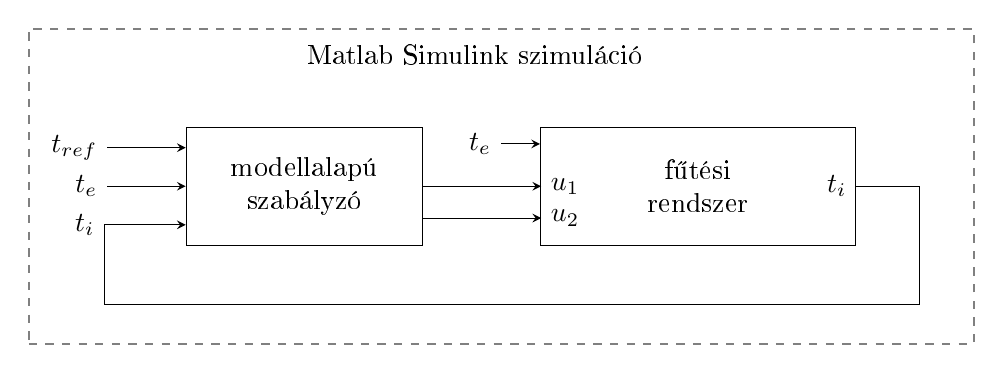
\begin{tikzpicture}[>=stealth,
	outer/.style={draw=gray,dashed,thick,inner sep=5pt}]
	
	% nagy blokkok
	\node[draw,rectangle, minimum height=1.5cm,minimum width=4cm] (plant) at (5,2.5) {\parbox{2cm}{\centering fűtési\\rendszer}};
	\node[draw,rectangle, minimum height=1.5cm,minimum width=3cm] (Control) at (0,2.5) {\parbox{2.5cm}{\centering modellalapú\\szabályzó}};
	
	% szaggatott vonal
	\node[draw,outer,rectangle, minimum height=4cm,minimum width=12cm,
	label={[label distance=-0.1cm, anchor=north]100:Matlab Simulink szimuláció}] (keret) at (2.5,2.5) {};
	
	
	% plant bemenetei
	\draw [->] (Control.0) node[right]{} -- +(15mm,0) node[right]{${u_{1}}$};
	\draw [->] (Control.345) node[right]{} -- +(15mm,0) node[right]{${u_{2}}$};
	\draw [<-] (plant.165) node[right]{} -- +(-5mm,0) node[left]{${t_{e}}$};
	%\draw [<-] (plant.90) node[right]{} -- +(0,3mm) node[right]{$t_{e}$};
	%\draw [<-] (plant.162) node[right]{} -- +(-10mm,0) node[left]{$t_{ref}$};
	
	% szabályzó bemenetei
	% a -| és |- máshogy fog törni, ha unconstraintelt.
	\draw [->] (plant.0)  node[left]{$t_i$} -|++(0.8,-1.5) -| ++(-9.25,0) |-  ++(-1.1,0) |- node[left]{$t_i$} (Control.198);
	
	\draw [<-] (Control.180) node[right]{} -- +(-10mm,0) node[left]{$t_{e}$};
	\draw [<-] (Control.162) node[right]{} -- +(-10mm,0) node[left]{$t_{ref}$};
	\end{tikzpicture}
	\caption{A szimuláció felépítése}
	\label{tikz:simulation-basic}
\end{figure}

%
\section{A szabályozás folyamata, szabályzótervezés}
A szabályzó a  modell alapján olyan szelepekkel képes beavatkozni, melyekkel a fűtőtestbe beáramló vízmennyiség  korlátozható. A szelepek ($u_1, u_2$) állását folytonosan tudom változtatni. A modell bemenetei a szelepek állásai és a külső hőmérséklet, kimenete a belső hőmérséklet ($t_i$).  A belső és külső hőmérsékletet mérem, a szabályzott jellemző a belső hőmérséklet.
%
A tervezés lépései a \textit{\ref{chap:ident}-\ref{chap:control}. fejezetben} olvashatóak.
%Az alapértelmezett paramétereket módosítom a fizikai korlátoknak megfelelően,  amelyek a beavatkozókra vagy a szakaszra vonatkoznak.
%
%Az MPC-nek rendkívül sok paraméterezési lehetősége van, amitől függően a szabályzás agresszívebb vagy robusztusabb lehet.   %---- (kazánok \cite[235.~o.]{Herz} szerint: kazánok hatásfoka, túlméretezése. )
%Az MPC szabályozás gyakorlati kipróbálásához fizikai tesztrendszert állítunk fel, itt az MPC tervezési kérdésekre koncentrálok, átviteli függvény modellből.
%
%
\section{Eredmények gyakorlati kipróbálása, további lehetőségek}
%
A szabályzótervezés lépéseit egy fizikai rendszerre is elvégzem, hogy további tapasztalatokat szerezzek. Végül áttekintem, hogy a szabályozás használatának milyen gyakorlati lehetőségei vannak, mind technikai értelemben, mind piacképesség szempontjából. Végül összefoglalom az elért eredményeket.


%, melynek paramétereit energetikai tanúsítványból vehetjük. Ezzel egy közelítő modelljét megkapjuk a háznak, terepi mérések nélkül is lehetséges a szabályzás. A telepítés ideje lecsökkenthető, hiszen a hosszas kalibrálás elmarad.  A modellezéshez külön írom fel a helyiség és a fűtőtestek modelljét.%Természetesen bevethetők zárt körben végzett identifikációs módszerek, adaptív szabályzók is.




%Ehhez először áttekintettem a hőátadás lehetséges formáit és forrásait.
%Ezután fűtőtestek modelljét állítom fel.




%\pagebreak

 %Arra jutottam, hogy ha a levegő hőmérsékletére szabályzok, akkor az abba beleszóló tényezőket veszem sorra:
%\begin{itemize}[noitemsep,topsep=0pt,parsep=0pt,partopsep=0pt]
%	\item konvektív hőátadás: a felszín közelében felmelegedett levegő áramlani kezd
%	\item radiatív hőátadás: sugárzással kibocsátott energia a környezetbe
%\end{itemize}

%\begin{figure}[h]
%	\centering
%	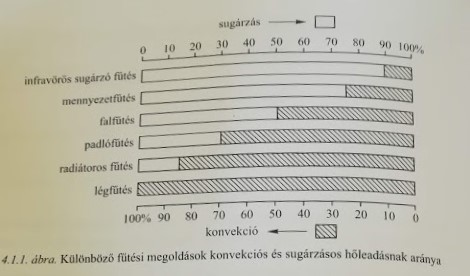
\includegraphics[width=8cm]{figures/konvrad}
%	\caption{Alacsony hőmérsékletű fűtés és magas hőmérsékletű hűtés c. könyv ábrája}
%		%\footnote{Jan Babiak, rehva Guidebook No.7}
%\end{figure}


%A levegő hőmérsékletére ezek a következőképp hatnak a leginkább:
%\begin{itemize}[noitemsep,topsep=0pt,parsep=0pt,partopsep=0pt]
%	\item a fűtőtestek konvektív és radiatív hőátadással is melegítik a környezetet
%	\item a radiatív energiát a tárgyak, falak nyelik el, amik ezáltal felmelegszenek (mintegy kapacitásként lesz egy hőtároló tömeg, ami a fűtés kikapcsolásával fenntartja a hőmérsékletet / lassítja a hűlést)
%	\item a fűtetlen falfelületek hűtik a szobát (külső hőmérséklet befolyása)
%\end{itemize}
%
%Így a kezdeti modellben azzal a feltételezéssel élek, hogy ezen kívül más hatás nem lép fel.
%
%A modellben feltételezem, hogy a fűtőtest felületi hőmérsékletével tudunk beavatkozni. A modellben paraméter a fűtőtestek hőátadási tényezője és felülete. Zavarásként (?) hat a külső hőmérséklet értéke, amit mérni is tudunk. Kimenet a belső hőmérséklet (térben konstansnak véve azt / átlagolva a szoba levegőjére)
%
%A modell felírásához a fűtőtest tulajdonságain kívül szükség van a szobában található levegő mennyiségére is. A zavarás hatását is fel kell írni, azaz hogy egy külső hőmérsékletváltozás hogyan jelenik meg a kimeneten. (Célszerű itt egy átviteli függvényt felírni először, szuperpozíciószerűen. A zavarás viszont nem a modell bemenetén és nem is a kimenetén hat.)

%A felírandó átviteli függvények:
%
%\begin{itemize}[noitemsep,topsep=0pt,parsep=0pt,partopsep=0pt]
%	\item levegő felmelegedése konstans külső hőmérsékletet feltételezve, fűtőtest egységugrással
%	\item levegő felmelegedése fűtés kikapcsolt állapota mellett, környezeti hőmérséklet ugrásával
%\end{itemize}
%
%Ezeket ráadtam a rendszerre és két bemenetű, egy kimenetű rendszerként identifikáltam.

%\pagebreak


%\subsubsection{Modellparaméterek}

%\subsection{-----}
%
%Fűtési típusok szerint:
%
%\begin{itemize}[noitemsep,topsep=0pt,parsep=0pt,partopsep=0pt]
%	\item radiátoros fűtés hőátvitele
%	\item padlófűtés hőátvitele
%\end{itemize}
%
%A fentiekre különböző értékű lesz a 
%
%\begin{itemize}[noitemsep,topsep=0pt,parsep=0pt,partopsep=0pt]
%	\item hőátadási tényező
%	\item hőtároló tömeg
%	\item költségfüggvény?
%	\item előremenő vízhőmérséklet és ezzel a leadott teljesítmény maximumértéke
%\end{itemize}
%
%ami így eltérő ház-modelleket fog eredményezni.


\pagebreak
\chapter{Helyiség modellje}\label{chap:helyiseg}

% Kiindulás ssc_house_heating_system

A szabályzótervezéshez rendelkezésre kell, hogy álljon a szabályozott szakasz modellje. Ezt két részre bontottam: először az épületszerkezet, azaz a helyiség modelljét írom fel, a fűtőtestekkel a \textit{\ref{chap:futotest}. fejezetben} foglalkozom. A \textit{\ref{fig:Simulink-minimalist}.~ábrán} látható a részekre bontott modell\footnote{A fűtőtestek teljesítménye függ a belső hőmérséklettől is (\textit{lásd \ref{eq_holeadas4}. egyenlet}), emiatt a modellben egy belső visszacsatolás található.}, melyből a helyiség alrendszert tárgyalom ebben a fejezetben. Egy könnyen módosítható, koncentrált paraméterű hálózatot vettem fel, ahol minden elemhez lehet fizikai tartalmat rendelni. A szabályzótervezéshez a teljes modell gerjesztés-válasz kapcsolatára lesz majd szükségem.
%todo footnote

Az energetikai jellemzők az épület energetikai tanúsítványából kiolvashatók, így a modell paraméterezhető. A tervezési lépéseket a névleges modellre elvégezve a szabályozás rögtön működőképes, nincs szükség hosszas kalibrációs időszakra beüzemelésnél. A modellbeli eltéréseket később kompenzálni lehet, mérési adatok felhasználásával.% (historikus adatok felhasználásával). %A modellben a bizonytalanságok hatása adaptív szabályozással kezelhető (lesz).

\begin{figure}[H]
	\centering
	% trim={<left> <lower> <right> <upper>}
	%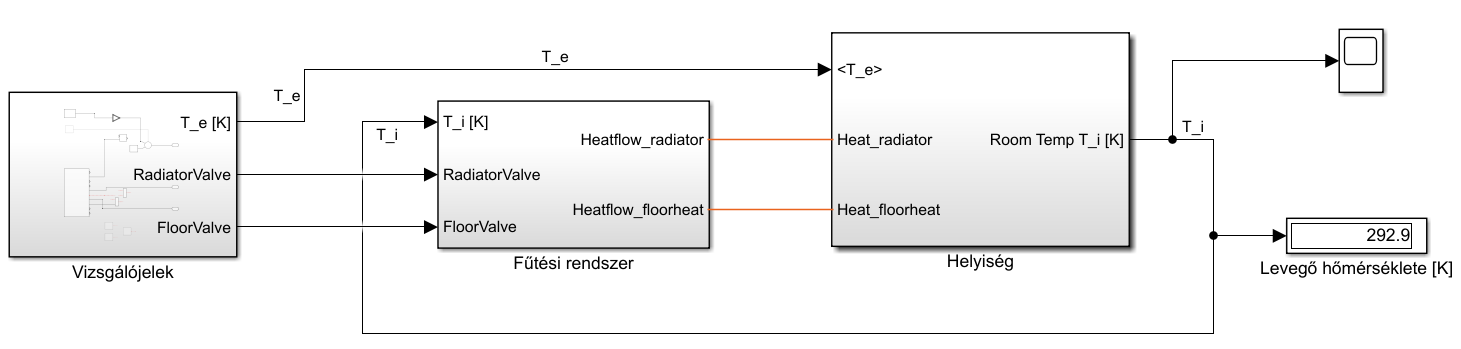
\includegraphics[trim=0 0 0 0, clip,width=\textwidth]{figures/simulink-network-minimalist-layout2}
	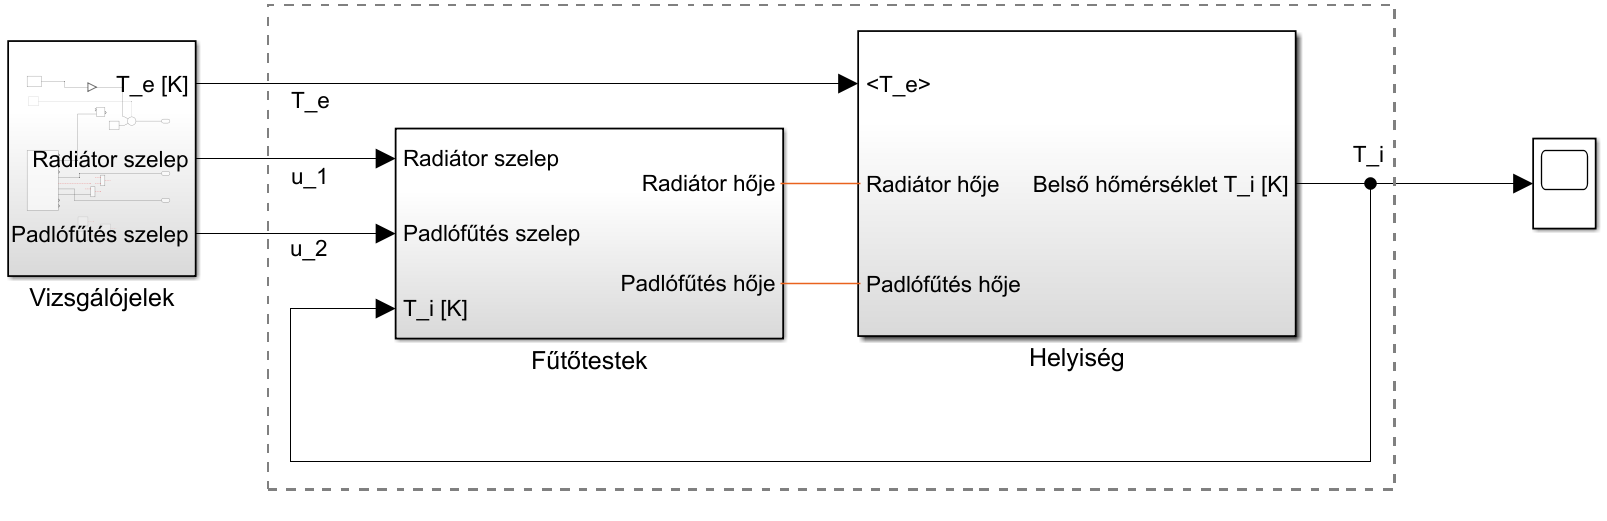
\includegraphics[trim=0 0 0 0, clip,width=\textwidth]{figures/simulink-network-minimalist-layout}
	\caption{Fűtési rendszer modellje - fűtőtest és helyiség}
	\label{fig:Simulink-minimalist}
\end{figure}

\section{A modellalkotás folyamata}
%
%White-box
%grey-box
%black-box

% zavarás, bemenet, nem irányított bemenet

A gerjesztés-válasz kapcsolatot megkaphatjuk méréssel, szimulációval vagy egyenletek felírásával. Mindegyik módszernek van előnye és hátránya is:  ha a hatásmechanizmusok pontosan ismertek, használhatunk "white-box" modellt, amiben fizikai összefüggések szerepelnek. Ha a hatásmechanizmus nem ismert, fekete dobozként ("black-box") is kezelhetjük a rendszert, de az identifikációhoz nagyon sok mérésre van szükség, hogy a mérési hibákat és zavarásokat kiküszöbölhessük.%\cite{THIEBLEMONT2017485}

Én a fizikai modell felírását választottam, melynek dinamikáját megvizsgálom a szabályozótervezéshez. Megfelelő gerjesztő jelekkel identifikálva előáll a modell átviteli függvénye (\textit{\ref{chap:ident}. fejezet}). Ehhez sokkal egyszerűbb eljutni, mint mérésekkel, mivel a Simulinkben megvalósított hálózatra az identifikáció sokkal egyszerűbb, mint valós rendszerre. A vizsgálójelek tetszőlegesen megválaszthatók, például a külső hőmérséklet hatása is pontosan meghatározható a \textit{\ref{fig:Simulink-minimalist}. ábrán} látható elrendezésben\footnote{Az átláthatóság kedvéért csak a kimenetet kötöttem rá a scope-ra, de a szimuláció közben az összes bemenetet, illetve belső változók állapotát is nyomon követhetjük.}. A helyiség egy MISO (több bemenetű, egy kimenetű) rendszer, terepi méréseket használva csak hosszas mérésekből lehet szétválasztani a bemenetek (fűtés, külső hőmérséklet és az ezekre ható zavarások) hatását a belső hőmérsékletre.



%Ha később páratartalom szabályzása is szóba kerül, még bonyolultabb a helyzet.


%\cite{SCHIRRER201686}

% --------------------------- kihúzva:
%A szakirodalomban pl. \cite{THIEBLEMONT2017485} és \cite{SCHIRRER201686} érinti ezt a kérdést:
%
%A szabályzótervezés során néhányan egyáltalán nem alkotnak modellt, csak a mért adatokat használják fel, ami eléggé időigényes: az identifikációhoz egy megfelelően nagy amplitúdójú vizsgálójelre van szükség. Viszont egy 10\si{\celsius}-kal felfűteni egy helyiséget hosszú ideig tart, ami alatt biztosan meg fog változni pl. a külső hőmérséklet. Ha a mérésekben a különböző inputok hatása a kimeneten nem különíthető el jó, az identifikáció nehéz lesz. Illetve külső hőmérséklet sem változik ugrásszerűen, a lassú időbeli változás \textit{nem jó vizsgálójel} identifikációhoz.
% ---------------------------

%Lényegében én is mért adatokat használok NEMMM, EZÉRT VAN A TANÚSÍTVÁNY!, tulajdonképpen, mivel a modellt olyan alakban kéne felírni, hogy a szabályzó azt futtatni tudja. (?)


% ---------------------------


%Vizsgálójel kiválasztása
%
%Modell struktúra kiválasztása - átviteli függvények pólusainak, zérusainak száma
%
%
%Viszont az ident toolbox tf identjénél kihasználtam azt, hogy a rendszer jellegét ismerem, azaz hogy hány pólusa és hány zérusa van a szakasznak  / felnyitott körnek. Így lett egy nagyon jól illeszkedő átviteli függvényem.
%
%Én összeraktam a fizikai modellt simulinkben (ez white-box) majd annak az ugrásválaszát mértem. Így nem egy állapotteres modell, hanem egy átviteli fv. "keletkezett".


Helyiségenkénti hőmérséklet-szabályozás esetén a belső hőmérsékletre adott egy referencia és egy mért érték.
Helyiségenként számos olyan tényező figyelembe vehető, melyek a teljes épületre különbözőek: a helyiség tájolása, az ablakok mérete, a felhasználás módja mind jobban kezelhető helyben, mint egy központi irányítással. Ezek mind-mind zavarásnak számítanak, ha pedig egy-egy helyiség hőmérsékletét mérjük, a zavarások ellenében ott tudunk beavatkozni, ahol azok hatnak. A helyi szabályozás referenciajeleit a lakók, dolgozók komfortérzetének megfelelően kell megadni.

A helyiség levegőjének hőmérsékletét mindenhol ugyanakkorának (homogénnek) feltételezem. A szabályozás a helyiség hőveszteségét egyenlíti ki, amit az alacsonyabb külső hőmérséklet okoz. Nem foglalkozok például szellőzésből, helyiségek közti hő\-mér\-sék\-let-különbségből\footnote{A modellezés egyszerűsítése végett több helyiség egymásra hatását nem veszem figyelembe.}, vagy emberek jelenlétéből származó belső zavarással.

A fűtést padlófűtés és radiátor biztosítja, mindkettőben szeleppel szabályozható az átfolyó vízmennyiség.

\section{A Simscape termikus elemei}

A \textit{\ref{fig:Simscape}. ábrán} látható egy termikus mintahálózat, mellyel bemutatom a Simscape csomag elemeit, melyből a helyiség modellje is felépíthető.

A források lehetnek fix hőmérsékletű elemek (feszültségforrás) illetve hőáram forrásai (áramforrás).
%A hasonlóság nem véletlen a villamos hálózatokkal. Felfedezhető, hogy a hőáramot a hőmérséklet-különbség hozza létre, nagysága pedig fordítottan arányos a hővezetési tényezővel. 
A "vezetékek" így azonos hőmérsékletű (ekvipotenciális) pontokat kötnek össze, ezekre hőmérsékletmérőket helyezhetünk. A különböző elemekkel sorba kapcsolva helyezhetők el hőáramlást mérő blokkok.

A hőáramlást a hőellenállások korlátozzák, mivel azokon hőmérsékletesés mérhető. (Az ábrán mért hőáram a hőellenálláson eső hőmérséklettel arányos, a \textit{\ref{eq_hoaram_alap}. egyenlet} szerint.) A hőtároló elemeknek tömege és fajhője megadja a hőkapacitásukat, így ezek feltöltődhetnek, energiát tárolhatnak.


A mintahálózat egy RC-tagnak felel meg, erre a szabályozótervezés lépései a következők lennének\footnote{Tekintsük a mintahálózatot és az itt részletezett lépéseket egy szemléletes példának, ugyanis a szakdolgozatban tárgyalt hálózatra is ezeken a lépéseken fogok végighaladni.}:

Az identifikációnál ismert a rendszer jellege, így 0 zérussal, 1 pólussal átviteli függvényt identifikálnék.
Erre szabályzót lehetne tervezni. A szimuláció során a termikus hálózat alapjele helyére kerülne a szabályzó beavatkozó jele. A visszacsatolás a hőmérő kimenetéről történne. Ilyen esetben, mivel a tervezés során használt modell és a  szakasz között nincs eltérés (angolul \textit{mismatch}), a szabályozás jól működik.
A paraméterek módosításával a szabályzó robusztussága tesztelhető.

Ha pedig ez a hálózat egy tényleges fizikai rendszer (például egy vízforraló) modellje lenne, akkor a szabályozás történhetne úgy, hogy a szabályzó Matlab-ban fut\footnote{A Matlab C kódot is képes generálni, ez is futtatható arra alkalmas eszközön, a számítógép nem feltétlenül szükséges.}, a hőmérsékletet mérjük, illetve a teljesítményelektronikán keresztül be tudunk avatkozni, így egy beállított hőmérsékletet tarthatunk.

\begin{figure}[H]
	\begin{subfigure}[t]{\textwidth}
		\centering
		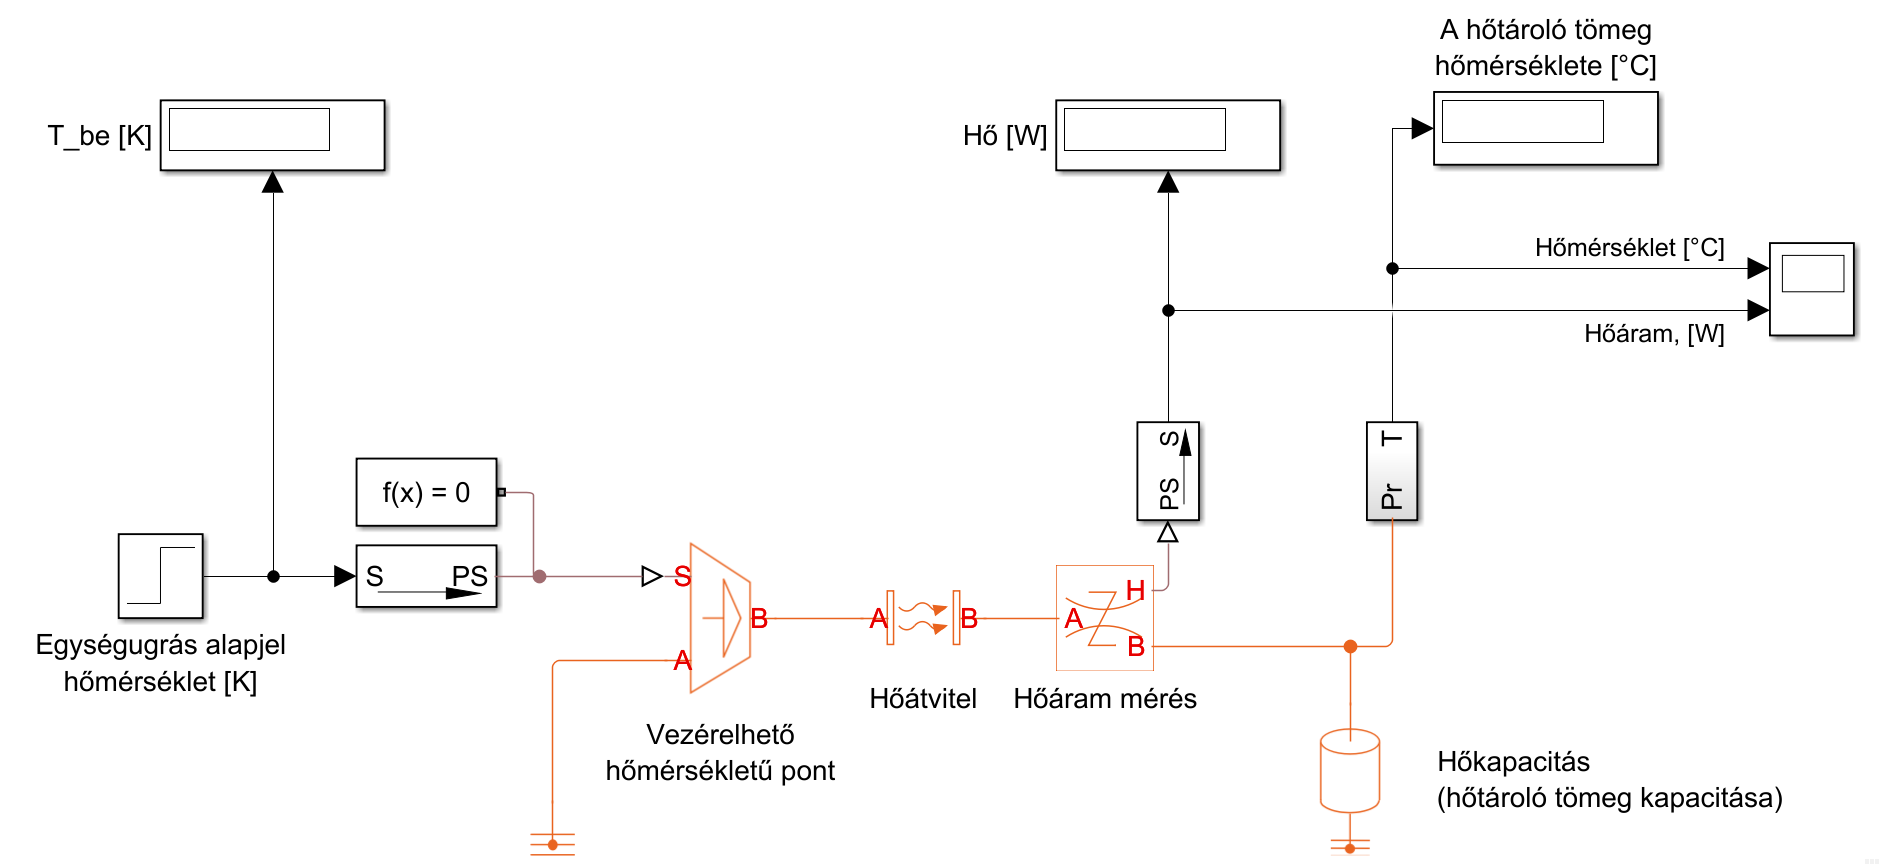
\includegraphics[width=\textwidth]{figures/SimscapeGeneral}
		\caption{Simscape termikus modell}
		\label{fig:SimscapeGeneral}
	\end{subfigure}%
	\smallskip
	\vspace*{10pt}
	\begin{subfigure}[t]{\textwidth}
		\centering
		% trim={<left> <lower> <right> <upper>}
		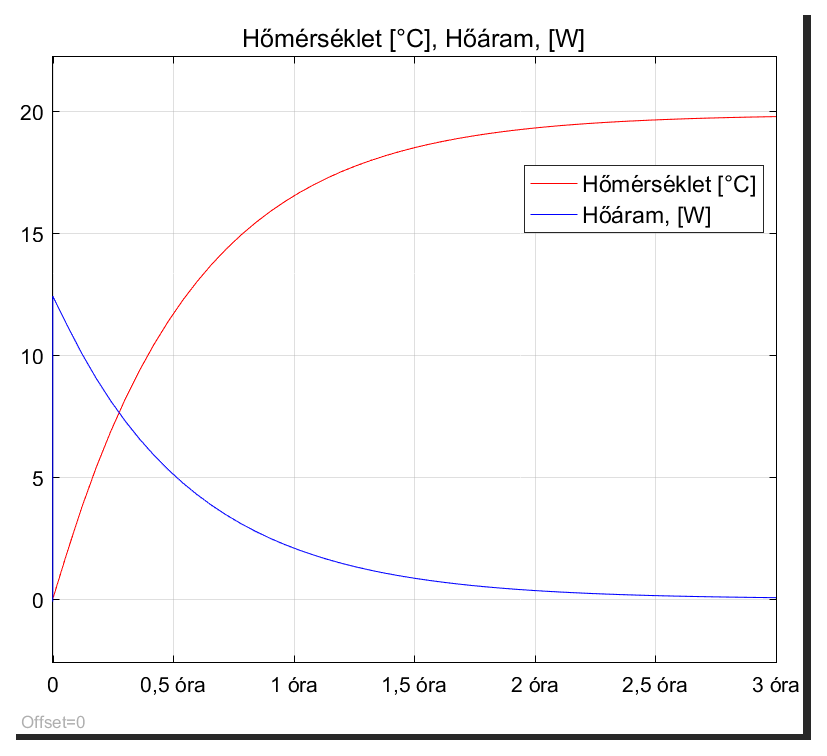
\includegraphics[trim=2 12 5 0, clip,width=0.49\textwidth]{figures/step_Simscape}
		\caption{Modell ugrásválasza}
		\label{fig:SimscapeStep}
	\end{subfigure}
	%	~
	%	\begin{subfigure}[t]{0.49\textwidth}
	%		\centering
	%%		\includegraphics[height=1.9in]{SSy}
	%%		\caption{Szimulált ugrásválasz}
	%%		\label{fig:SSy}
	%	\end{subfigure}	
	\caption{Tranziens (instacioner) hőtranszfer modellezése}
	\label{fig:Simscape}
	\centering
\end{figure}


%Természetesen lehetett volna nagyon sok állapotú állapoteres modellt is létrehozni, ám rengeteg nem mérhető belső változója lett volna, emiatt nem biztos hogy teljesen irányítható vagy megfigyelhető rendszert kaptam volna, így pedig a szabályzótervezés nem működik.


 
% \textbf{ÁBRA WHITE-BOX MODELRŐL, ÉS BLACKBOX IDENTIFIKÁCIÓRÓL. ILLETVE WHITEBOX IDENT.}


\section{Épületfizikai alapösszefüggések}
 
 A Simscape modell felépítéséhez szükség van néhány alapösszefüggésre.
 
 Különböző hőmérsékletű testek közötti energiaátmenetet hőátvitelnek
 (hőtranszportnak) nevezzük. A magasabb hőmérsékletű
 test (a termodinamika második főtételének értelmében) átadja hőjének
 egy részét az alacsonyabb hőmérsékletű testnek.
A hőátvitelnek három alapvető formája van, a hővezetés (kondukció), a hőáramlás (konvekció) és a hősugárzás (radiáció)\footnote{A hőátvitel definíciójának forrása: Dr. Fekete Iván, Épületfizika kézikönyv}.
 

\begin{table}[H]
	\footnotesize
	\centering
	%\renewcommand{\arraystretch}{2} % to increase cell height
	%\taburulecolor{gray}
	%\begin{tabular}{|p{0.8cm}|p{1cm}|p{1cm}|p{1cm}|p{1cm}|p{1cm}|p{1cm}|p{1cm}|}
	%
	\newcolumntype{C}[1]{>{\centering\arraybackslash}p{#1}}
\newcolumntype{R}[1]{>{\raggedleft\arraybackslash}p{#1}}


\begin{tabu}{p{1.5cm}C{1.6cm}C{7cm}C{4cm}}
	%{p{1.5cm}|C{0.8cm}|C{0.8cm}|C{0.8cm}|C{0.8cm}|C{0.8cm}|C{0.8cm}|C{0.8cm}|C{0.8cm}|}
	%\multicolumn{1}{l}{}&\multicolumn{8}{l}{SDO header (első adatbyte) - master kérése}
	%\\ 		\cline{2-9}\cline{2-9}
	\hline
	\\
	& együtthatója &  a hőátadás szereplői & példa
	\\
	konvektív &  $\lambda$& áramló közeg -- szilárd anyag felülete & levegő vagy víz áramlása
	\\
	konduktív &  $h_c$&  az anyag molekulái között & az anyag belsejében
	\\
	radiatív &  $h_r$& tárgyak között, felszínükkel arányosan & hősugárzás 
	\\
%	& méret & $h_t$, átlag    & hőtároló tömeg & hőkapac
%	\\
%	& méret & $h_t$, átlag    & hőtároló tömeg & hőkapac
%	\\
%	& méret & $h_t$, átlag    & hőtároló tömeg & hőkapac
%	\\
%	& méret & $h_t$, átlag    & hőtároló tömeg & hőkapac
%	\\
%	& méret & $h_t$, átlag    & hőtároló tömeg & hőkapac
%	\\ %\hline
%	külső fal & 4.5 \si{\metre\squared} & 2 \si[per-mode=fraction]{\watt\per\metre\squared\per\kelvin} & 900kg & 756 \si[per-mode=fraction]{\kilo\joule\per\kelvin}
%	\\ %\hline
%	ablak & 4 \si{\metre\squared} & 4 \si[per-mode=fraction]{\watt\per\metre\squared\per\kelvin} & 0 & 0
%	\\ %\hline
%	belső válaszfalak & 50 \si{\metre\squared} & 7 \si[per-mode=fraction]{\watt\per\metre\squared\per\kelvin} & 5000kg & 4.2 \si[per-mode=fraction]{\mega\joule\per\kelvin}	
%	\\ %\hline
%	padló & 16 \si{\metre\squared} & 11 \si[per-mode=fraction]{\watt\per\metre\squared\per\kelvin}  & 3200kg &2.7 \si[per-mode=fraction]{\mega\joule\per\kelvin}
%	\\ %\hline
%	mennyezet & 16 \si{\metre\squared} & 5 \si[per-mode=fraction]{\watt\per\metre\squared\per\kelvin} & 3200kg &2.7 \si[per-mode=fraction]{\mega\joule\per\kelvin}	
	\\ \hline

%	belső válaszfalak & 50 \si{\metre\squared} & 7 & 50*100kg & 50*100*840		
%	\\ \hline
%	11 & Internal limit active
%	\\ \hline
%	12-13 & Operation mode specific
%	\\ \hline
%	14-15 & Reserved
\end{tabu}

	\caption{Hőközlés fajtái}
	\label{tab:HeatExchangeTypes}
	%
	%\label{tab:TabularExample}
	%\tabref{TabularExample}~táblázat
\end{table}

\subsection{Hővezetés}

A hővezetés alapegyenlete:

\begin{equation} \label{eq_hovezetes}
\begin{aligned}
Q = A \frac{\lambda}{d} \Delta T
\end{aligned}
\end{equation}

Ezzel falszerkezeteken keresztüli hőáramot tudjuk megadni. Minden rétegre ismernünk kell a hővezetési tényezőt és a vastagságot.

Több réteg és a levegő hatása együttesen is kezelhető a rétegrendi hőátbocsátási tényezővel: fal esetén annak két oldalán található levegő hőátadási tényezőjét is figyelembe veszi. Külső fal esetén így a hőveszteség felírható a belső és külső levegő hőmérsékletének függvényében. 

\begin{equation}\label{eq_hoatbcsatas_U}
\begin{aligned}
U = \frac{1}{\frac{1}{\alpha_e}+\sum\limits_{i}^{}\frac{d_i}{\lambda_i}+\frac{1}{\alpha_i}}\\[10pt]
Q = AU(t_i - t_e)
\end{aligned}
\end{equation}

\subsection{Sugárzó és konvektív hőátadás}

A hőáramlás (konvekció) alapegyenlete:

\begin{equation} \label{eq_konvektiv}
\dot Q_{le} = h_c ~ A ~ (t_{surf} - t_i)
\end{equation}


A \textit{REHVA Guidebook} \cite{RehvaGuidebookNo7} címében is szerepel az \textit{alacsony hőmérsékletű fűtés} fogalma. Ez nem paradoxon, csupán azt jelenti, hogy a fűtőfelületek hőmérséklete az átlagosnál alacsonyabb. A levegőnél csak néhány fokkal magasabb hőmérsékletű fűtési rendszerekben pedig alacsonyabb lehet az előremenő vízhőmérséklet. Megújuló energiát használó rendszerekre ez előnyösebb, mint a régi, széntüzelésű kazánok által előállított 80--\SI{90}{\celsius}-os előremenő vízhőmérséklet.

A kis hőmérsékletkülönbség következménye, hogy a levegőnek csak kevés hőt képes leadni a rendszer. Nagyobb részt sugárzással működnek ezek a rendszerek, melyet a fűtetlen felületek nyelnek el. Ezért sugárzó (radiatív) hőátvitel esetén szokásos a $t_{AUST}$ jelölés, ami a fűtetlen felületek hőmérsékletét jelenti\footnote{AUST: Average unheated surface temperature, azaz a fűtetlen felületek átlagos hőmérséklete}.

A sugárzási hőtranszfer alapegyenletét a Stefan-Boltzmann törvény adja


\begin{equation} \label{eq_stefan_boltzmann}
\begin{aligned}
\dot Q_{r} &= \sigma T_{surf}^4
\end{aligned}
\end{equation}

ahol
\begin{itemize}[itemsep=9pt,topsep=0pt,parsep=0pt,partopsep=0pt]
	\item[] $\sigma$ a Stefan-Boltzmann állandó [\si{W~m^{-2}.K^{-4}}] %\si[per-mode=fraction]{W/m^2K^4}% \si[per-mode=fraction]{\watt\per\metre\squared\per\kelvin\squared\squared} %eh [\si[per-mode = fraction]{\watt\per\metre\squared\per\kelvin^4}]
	\item[] $T_{surf}$ [\si{\kelvin}] a termodinamikai, azaz kelvinben mért felületi hőmérséklet.
\end{itemize}


(\textit{Kilkis} \cite{KILKIS1994} ):

\begin{equation} \label{eq_radiant_kilkis}
\begin{aligned}
\dot Q_{r} &= U_r ~ A~ \left(t_{surf}-t_{AUST}\right)\\[8pt]
U_r&=rF\sigma\\
r&=4 \left(\frac{T_{surf}}{2}+\frac{T_{AUST}}{2}\right)^3
\end{aligned}
\end{equation}


ahol
\begin{itemize}[itemsep=9pt,topsep=0pt,parsep=0pt,partopsep=0pt]
	\item[] $T_{surf}, T_{AUST}$ [\si{\kelvin}] a termodinamikai, azaz kelvinben mért hőmérséklet.
	\item[] $c$ [\si[per-mode = fraction]{\joule\per\kg\per\kelvin}] a víz fajhője
	%	\item[] $\xi$ a szabályzó beavatkozó jele, $ \xi \in [0,1]$ folytonosan változhat 0 és 1 között
	%	\item[] $\dot{m}$ [\si[per-mode = fraction]{\kg\per\second}] a víz tömegárama
	%	\item[] $\Delta t = t_w-t_r$ [\SI{}{\kelvin}] a víz lehűlésének mértéke
\end{itemize}

A sugárzó hőleadási tényező bevezetésével linearizálhatjuk a hőleadást, a hőleadás így egyszerűen lineárisan függ majd a hőmérséklet-különbségtől. Gyakran összevonják a konvektív és a sugárzási hőátadási tényezőt. Én is így használom fel ezeket a padlófűtés modelljében: a felmelegedett padló sugárzással adja át a hőt a falaknak és a mennyezetnek. 

\textit{Cholewa} \cite{CHOLEWA2013599} a $h_r$ paramétert méréssel határozta meg, amivel ezután az alábbi formában számolható a sugárzó hő mennyisége:



\begin{equation} \label{eq_radiative_hr_linear}
\dot Q_{r} = h_r ~ A ~ \left(t_{surf}-t_{AUST}\right)
\end{equation}

ahol
\begin{itemize}[itemsep=3pt,topsep=0pt,parsep=0pt,partopsep=0pt]
	\item[] $\dot{Q}_{r}$ [\SI{}{\watt}] a leadott sugárzó hő
	\item[] $h_r$ [\si[per-mode = fraction]{\watt\per\meter\squared\per\kelvin}] sugárzó hőleadási tényező
	\item[] $A$ [\si{\metre\squared}] a padló felülete
	\item[] $t_{surf}$ [\SI{}{\kelvin}] padló hőmérséklete
	\item[] $t_{AUST}$ [\SI{}{\kelvin}] fűtetlen felületek átlagos hőmérséklete - a fal hőmérsékletének veszem a Simscapeben
\end{itemize}


\subsubsection*{Hőtároló képesség}


Falszerkezeteknél annak hőtároló képessége adja meg, hogy \SI{1}{\celsius}-os hőmérséklet-változás esetén mennyivel változik a szerkezet energiája.

Az \textit{EN ISO 13790} szerint az épület hőtároló tömege az épület belső levegőjével közvetlen kapcsolatban lévő határolószerkezetek hőtároló tömegének összege.

\begin{equation}\label{eq_hotarolo-tomeg}
\begin{aligned}
M= \rho d A\\[10pt]
\Delta Q= cM\Delta t
\end{aligned}
\end{equation}

Ebben az esetben eltérek a szabványban használt módszerektől. Az \textit{MSZ 24140} megadja, hogy egyes anyagoknál mekkora réteget kell figyelembe venni egy napos ciklusidejű hőtárolásra. Ez azért nem pontos, mert több napos átmelegedési időkkel nem számol. Az energetikai tanúsítványok azonban tartalmazzák a teljes tömeget és a szabvány szerinti hőtároló tömeget is. A modellben a teljes tömeg szerepel.




\begin{table}[H]
	\footnotesize
	\centering

	%\renewcommand{\arraystretch}{2} % to increase cell height
	%\taburulecolor{gray}
	%\begin{tabular}{|p{0.8cm}|p{1cm}|p{1cm}|p{1cm}|p{1cm}|p{1cm}|p{1cm}|p{1cm}|}
	%
	\newcolumntype{C}[1]{>{\centering\arraybackslash}p{#1}}
\newcolumntype{R}[1]{>{\raggedleft\arraybackslash}p{#1}}

\setstretch{1.8}

\begin{tabulary}{\linewidth}{LLc}
	%\begin{tabulary}{|p{3cm}|p{1.2cm}|p{2cm}|p{3cm}|p{3cm}|}
	%{p{1.5cm}|C{0.8cm}|C{0.8cm}|C{0.8cm}|C{0.8cm}|C{0.8cm}|C{0.8cm}|C{0.8cm}|C{0.8cm}|}
	%\multicolumn{1}{l}{}&\multicolumn{8}{l}{SDO header (első adatbyte) - master kérése}
	%\\ 		\cline{2-9}\cline{2-9}
	\hline
	${Q}_{total} $& hőáram 				& \si[per-mode=fraction]{\watt} = \si[per-mode=fraction]{\joule\per\second}
	\\
	$A $		& felszín				& \si[per-mode=fraction]{\watt\per\metre\squared}
	\\
	$U$ 		& réteges szerkezet hőátbocsátási tényezője  & \si[per-mode=fraction]{\watt\per\metre\squared\per\kelvin}
	\\
	$q_{total} $& teljes hőáramsűrűség 	& \si[per-mode=fraction]{\watt\per\metre\squared}
	\\
	$h_{total}$	& teljes hőcsere együttható & \si[per-mode=fraction]{\watt\per\metre\squared\per\kelvin}
	\\
	$h_{r}$ 	& radiatív hőátadási tényező & \si[per-mode=fraction]{\watt\per\metre\squared\per\kelvin}
	\\
	$h_{c}$, $\alpha$
				& konvektív hőátadási tényező
										& \si[per-mode=fraction]{\watt\per\metre\squared\per\kelvin}
	\\
	$\lambda$  	& konduktív hőátadási tényező & \si[per-mode=fraction]{\watt\per\metre\squared\per\kelvin}
	\\
	$\varepsilon$
				& emisszivitás & --
	\\
	$t_{ref}$ 	& referencia hőmérséklet& \si[per-mode=fraction]{\celsius}
	\\
	$t_i$ 		& belső hőmérséklet 	& \si[per-mode=fraction]{\celsius}
	\\
	$t_e$ 		& külső hőmérséklet 	& \si[per-mode=fraction]{\celsius}
	\\
	$c$ 		& fajhő 		& \si[per-mode=fraction]{\joule\per\kilogram\per\kelvin}
	\\
	$C$		& hőkapacitás 		& \si[per-mode=fraction]{\joule\per\kelvin}
	\\
	$\dot{m}$ 	& tömegáram 	& \si[per-mode=fraction]{\kilogram\per\second}
	\\
	$\xi$, $u_1,u_2$
				& szelep kinyitásának mértéke [0..1]				& $\%$
	\\
	$\Delta t_m$& közepes hőmérsékletkülönbség 	& \si[per-mode=fraction]{\celsius}
	\\
	$t_i$ 		& belső hőmérséklet 	& \si[per-mode=fraction]{\celsius}

%	& méret & $h_t$, átlag    & hőtároló tömeg & hőkapac
%	\\
%	& méret & $h_t$, átlag    & hőtároló tömeg & hőkapac
%	\\
%	& méret & $h_t$, átlag    & hőtároló tömeg & hőkapac
%	\\
%	& méret & $h_t$, átlag    & hőtároló tömeg & hőkapac
%	\\
%	& méret & $h_t$, átlag    & hőtároló tömeg & hőkapac
%	\\ %\hline



%	külső fal & 4.5 \si{\metre\squared} & 2 \si[per-mode=fraction]{\watt\per\metre\squared\per\kelvin} & 900kg & 756 \si[per-mode=fraction]{\kilo\joule\per\kelvin}
%	\\ %\hline
%	ablak & 4 \si{\metre\squared} & 4 \si[per-mode=fraction]{\watt\per\metre\squared\per\kelvin} & 0 & 0
%	\\ %\hline
%	belső válaszfalak & 50 \si{\metre\squared} & 7 \si[per-mode=fraction]{\watt\per\metre\squared\per\kelvin} & 5000kg & 4.2 \si[per-mode=fraction]{\mega\joule\per\kelvin}	
%	\\ %\hline
%	padló & 16 \si{\metre\squared} & 11 \si[per-mode=fraction]{\watt\per\metre\squared\per\kelvin}  & 3200kg &2.7 \si[per-mode=fraction]{\mega\joule\per\kelvin}
%	\\ %\hline
%	mennyezet & 16 \si{\metre\squared} & 5 \si[per-mode=fraction]{\watt\per\metre\squared\per\kelvin} & 3200kg &2.7 \si[per-mode=fraction]{\mega\joule\per\kelvin}	
	\\ \hline
%	belső válaszfalak & 50 \si{\metre\squared} & 7 & 50*100kg & 50*100*840		
%	\\ \hline
%	11 & Internal limit active
%	\\ \hline
%	12-13 & Operation mode specific
%	\\ \hline
%	14-15 & Reserved
\end{tabulary}

	\caption{Jelölések}
	\label{tab:Nomenclature}
	%
	%\label{tab:TabularExample}
	%\tabref{TabularExample}~táblázat
\end{table}

\section{A megvalósított modell}

Figyelembe kell vennem a ház hőveszteségeit és hőtároló képességét is, a \textit{\ref{eq_hotarolo-tomeg}. egyenlet} alapján, melynek paraméterei a \ref{table_house_parameters}. táblázatban találhatók.
Az alábbi táblázat értékeinek nagy részét ki lehet tölteni a tanúsítványból. Feltételezem, hogy ez rendelkezésre áll, hiszen ennek elkészítésére elég sok esetben szükség van (adásvétel, felújítás, stb.).
Az épület éves hőigénye numerikusan is szerepel a tanúsítványban. Itt a fűtési rendszer tulajdonságain kívül a várható napsütéses órák számát és a használati melegvíz előállításának energiaigényét figyelembe veszi\footnote{A hőigény számításához törvényi előírások alapján különböző korrekciós tényezőket használnak.}.
%TODO hol van ez a törvényben?

A Matlab Simscape model és \textit{Lapusan} \cite{LAPUSAN2016320}
%\footnote{Development of a Multi-Room Building Thermodynamic Model Using Simscape Library - Ciprian Lapusan}
 hőátadásnál a réteges szerkezetekben számolt konvekcióval és kondukcióval is. Viszont ezek az adatok egyben is kezelhetők, a követelményeket ezekre a költségoptimalizált követelményszint\footnote{ A  költségoptimalizált követelményszintek megtalálhatók a 7/2006. rendelet \cite{TNM2006} 5. mellékletében.} adja meg. Régebbi épületek ezt a szintet nem tudják teljesíteni, ezekre jellemző értékeket adtam meg az alábbi táblázatban. 
%todo táblázat

Ám nem szabad összekeverni a külső falakra vonatkozó U értéket (rétegrendi hőátbocsátási tényező) és az $h_c$ konvektív hőátadási tényezőt, amit a válaszfalakra, padlóra és mennyezetre adtam meg, hiszen ezeken a modell szerint a helyiség nem veszt hőt, csak a hőtároló elemeknek adódik át.

 A példában a Schönherz Zoltán Kollégium egy szobájának megfelelő méretű helyiséget vettem fel. Minden szobának van ablaka és külső fala, egy átlagos szobát 4 másik vesz körül. A belső falakon nem veszt hőt, csak az ablakon ill. a külső falon. Feltételezzük, hogy a radiátoros fűtést egy szeleppel szabályozhatjuk, amit tetszőleges mértékben nyithatunk ki.
 %A napsütés hőnyereségét is figyelembe vehetjük.%, úgy, hogy egy hőforrás a padlót melegíti.

\begin{figure}[H]
	\centering
	% trim={<left> <lower> <right> <upper>}
	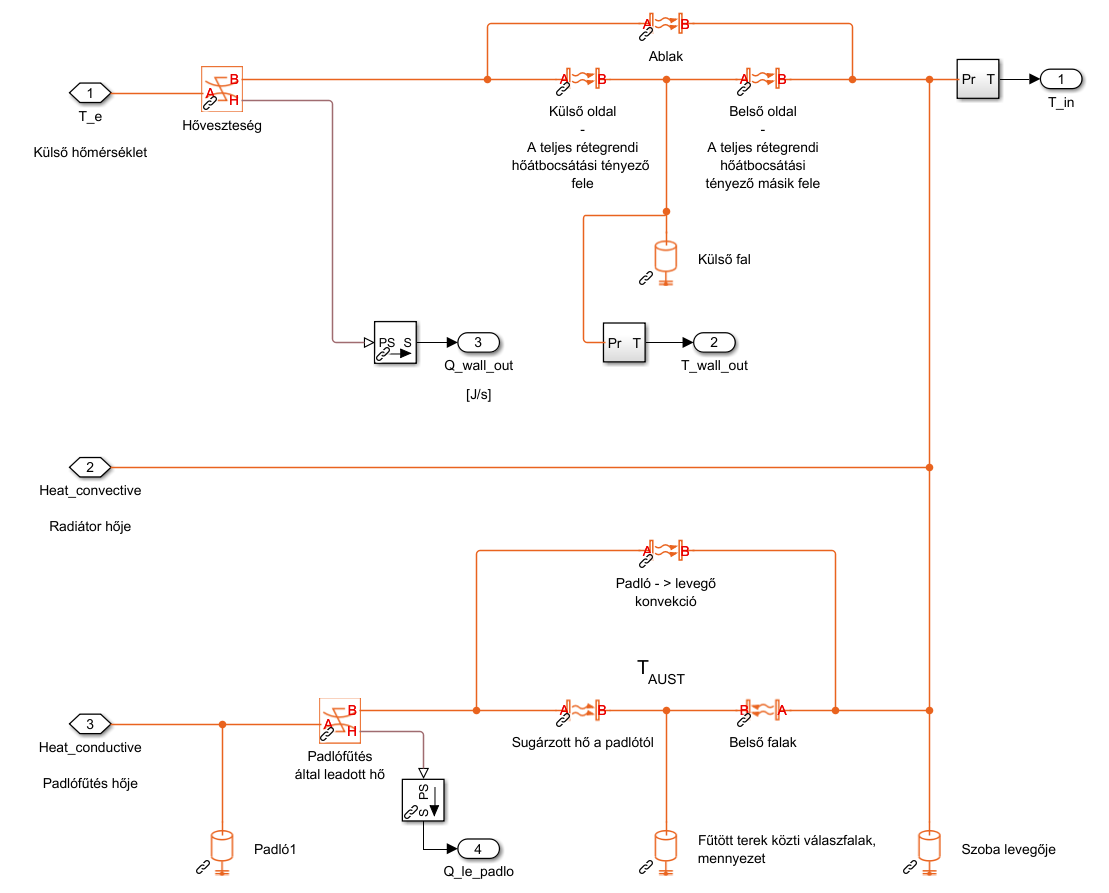
\includegraphics[trim=0 12 5 0, clip,width=\textwidth]{figures/SimscapeHouse}
	\caption{Helyiség termikus modellje}
	\label{fig:SimscapeHouse}
\end{figure}

A helyiség modellje a \textit{\ref{fig:SimscapeHouse}. ábrán} látható, három bemenete van: külső hőmérséklet, radiátor hője és a padlófűtés hője.
A külső hőmérséklet egy \say{feszültség jellegű} bemenet, hőáramot nem szab meg.
A radiátor \say{áram jellegű} kimenetet ad, hiszen itt a képlet a leadott hőt számítja: a radiátor konduktív hőárama közvetlenül a levegőt melegíti. A padlófűtés először a padlónak adja át a hőt, utána pedig a levegőnek (konduktív hőátadás), illetve a falaknak (sugárzó, radiatív hőátadás).

A levegőnek, padlónak, falaknak tömegüknél és fajhőjüknél fogva mind-mind van egy hőtároló képességük (\textit{\ref{table_house_parameters}. táblázat}), egy bizonyos idő alatt tudnak feltöltődni vagy hőenergiájukat leadni: hőmérsékletük nem változhat ugrásszerűen. %Mindezekben villamosmérnöki szemszögből felfedezhetjük az analógiát a villamos hálózatokkal.


\begin{table}[H]
	\footnotesize
	\centering

	\renewcommand{\arraystretch}{1.3} % to increase cell height
	\taburulecolor{gray}
	%\begin{tabular}{|p{0.8cm}|p{1cm}|p{1cm}|p{1cm}|p{1cm}|p{1cm}|p{1cm}|p{1cm}|}
	\caption{A helyiség hőveszteséget okozó elemei}
	\newcolumntype{C}[1]{>{\centering\arraybackslash}p{#1}}
\newcolumntype{R}[1]{>{\raggedleft\arraybackslash}p{#1}}
\begin{tabu}{@{}p{3.5cm}p{1.2cm}p{2cm}p{3cm}p{3cm}@{}}
	%\begin{tabu}{|p{3cm}|p{1.2cm}|p{2cm}|p{3cm}|p{3cm}|}
	%{p{1.5cm}|C{0.8cm}|C{0.8cm}|C{0.8cm}|C{0.8cm}|C{0.8cm}|C{0.8cm}|C{0.8cm}|C{0.8cm}|}
	%\multicolumn{1}{l}{}&\multicolumn{8}{l}{SDO header (első adatbyte) - master kérése}
	%\\ 		\cline{2-9}\cline{2-9}
	veszteséges elemek& méret & $U$    & hőtároló tömeg & hőkapacitás
	\\ \hline%\hhline{=====}
	külső fal & 4.5 \si{\metre\squared} & 2 \si[per-mode=fraction]{\watt\per\metre\squared\per\kelvin} & 900kg & 756 \si[per-mode=fraction]{\kilo\joule\per\kelvin}
	\\ %\hline
	ablak & 4 \si{\metre\squared} & 4 \si[per-mode=fraction]{\watt\per\metre\squared\per\kelvin} & - & -
	\\ %\hline
\end{tabu}

%	\begin{subtable}
%		\newcolumntype{C}[1]{>{\centering\arraybackslash}p{#1}}
\newcolumntype{R}[1]{>{\raggedleft\arraybackslash}p{#1}}


\begin{tabu}{@{}p{3.5cm}p{1.2cm}p{2cm}p{3cm}p{3cm}@{}}
	csak hőtároló elemek & méret & $h_t$    & hőtároló tömeg & hőkapacitás \\	\hline%\hhline{=====}
	belső válaszfalak & 50 \si{\metre\squared} & 7 \si[per-mode=fraction]{\watt\per\metre\squared\per\kelvin} & 5000kg & 4.2 \si[per-mode=fraction]{\mega\joule\per\kelvin}	
	\\ %\hline
	padló & 16 \si{\metre\squared} & 11 \si[per-mode=fraction]{\watt\per\metre\squared\per\kelvin}  & 3200kg &2.7 \si[per-mode=fraction]{\mega\joule\per\kelvin}
	\\ %\hline
	mennyezet & 16 \si{\metre\squared} & 5 \si[per-mode=fraction]{\watt\per\metre\squared\per\kelvin} & 3200kg &2.7 \si[per-mode=fraction]{\mega\joule\per\kelvin}	
	\\ %\hline
\end{tabu}

%	\end{subtable}
	\label{table_house_parameters}
	%\label{tab:TabularExample}
	%\tabref{TabularExample}~táblázat
\end{table}

\begin{table}[H]
	\footnotesize
	\centering

	\renewcommand{\arraystretch}{1.3} % to increase cell height
	\taburulecolor{gray}
	\newcolumntype{C}[1]{>{\centering\arraybackslash}p{#1}}
\newcolumntype{R}[1]{>{\raggedleft\arraybackslash}p{#1}}


\begin{tabu}{@{}p{3.5cm}p{1.2cm}p{2cm}p{3cm}p{3cm}@{}}
	csak hőtároló elemek & méret & $h_t$    & hőtároló tömeg & hőkapacitás \\	\hline%\hhline{=====}
	belső válaszfalak & 50 \si{\metre\squared} & 7 \si[per-mode=fraction]{\watt\per\metre\squared\per\kelvin} & 5000kg & 4.2 \si[per-mode=fraction]{\mega\joule\per\kelvin}	
	\\ %\hline
	padló & 16 \si{\metre\squared} & 11 \si[per-mode=fraction]{\watt\per\metre\squared\per\kelvin}  & 3200kg &2.7 \si[per-mode=fraction]{\mega\joule\per\kelvin}
	\\ %\hline
	mennyezet & 16 \si{\metre\squared} & 5 \si[per-mode=fraction]{\watt\per\metre\squared\per\kelvin} & 3200kg &2.7 \si[per-mode=fraction]{\mega\joule\per\kelvin}	
	\\ %\hline
\end{tabu}

	\label{table_house_parametersB}
	\caption{A helyiség veszteségmentes elemei}
\end{table}

A falak hőtároló tömegénél a teljes válaszfal tömegének csak a felét vettem figyelembe, a másik fele egy másik helyiséghez tartozhat. A fenti értékek becslések, az energetikai tanúsítványban pontosan szerepelnek ezek az értékek is.

%A modell mintavételi ideje?
%A teljesítményeket megnöveljük és semmi mást, az nem lesz ekvivalens. 

\subsubsection*{Hőigény:}

A külső falon

\begin{equation}\label{eq_hoigeny}
\begin{aligned}
		Q_{ki,fal} &= U_{fal}A_{fal}\Delta T = 200\si{\watt}\\[10pt]
		Q_{ki,ablak} &= U_{ablak}A_{ablak}\Delta T = 400\si{\watt}
\end{aligned}
\end{equation}

Amennyiben a méretezési hőmérséklet $\Delta T=$ \SI{-2}{\celsius}, ami a téli átlaghőmérséklet Magyarországon. Ezeket az adatokat fogom méretezéskor figyelembe venni.
%TODO honnan \footnote{Épületfizika kurzus alapján vettem az átlaghőmérsékletet \SI{-2}{\celsius}-nak.}


%(Gondolatkísérlet: HA nem hatna zavarás, csak az időállandók számítanának, a pontos teljesítményveszteségek, nyereségek nem. Azaz mindegy volna hogy 1000W hő szökik ki és ehhez tartozik 1500W-nyi fűtési kapacitás, vagy hogy 5000W és 7500W ezek az értékek. Ám pl. napsütés hatásakor nem csak az arányok hanem a konkrét teljesítmények is kellenek...

%Így a modell egyik belső változója bizonyosan a teljesítmény kell, hogy legyen. Erre a belső változóra hat majd zavarás: emberek jelenléte kb. \SI{80}{\watt} 1 főre, napsütés, szellőztetés, stb.)

%\hrulefill


%Erre ki kellene számítani a hőigényt, figyelembe véve azt hogy mennyi hő szökik el a külső és belső határoló felületeken keresztül.
%A gyakorlati alkalmazásokban szeretnék majd az energetikai tanúsítványból kiindulni.%, így gyakorlatilag a szoba energetikai tanúsítását végzem el - olyan szinten, amennyire nekem szükséges.


%Ashrae HVAC - 6.19 Panel H \& C. - Controls strategy
%
%A modellt a jellemző szerkezeti tulajdonságok alapján írtam fel (indoklás a táblázathoz). A modellezés Gouda alapján történik, gyakorlatilag csomóponti egyenleteket kell felírni az alábbi hálózatra, amiben az ellenállások a rétegrendi hőátbocsátási tényező reciprokai. A hőtároló képességeket kapacitások modellezik. Ezeket az elemeket Simscape-ben implementáltam, a hőáramok így áttekinthetők és a paraméterek könnyen változtathatók.
%
%A ház modelljének felírásakor figyelembe vettem a hőtároló elemeket. A pontos (reális) modell felállításakor ezek hőtartalmát (a hőáram integrálja egyensúlyi állapotban legyen 0, azaz egy nagyobb ciklusban a felvett és leadott hője egyenlő) az egyensúlyi állapothoz közelinek vettem.
%
%Viszont a szabályzótervezéshez identifikálni kell, ekkor pedig a falak, ill. szoba levegőjének kezdeti állapotát (hőmérsékletét) azonosnak vettem a külső hőmérséklettel. Így ha a hőkülönbség a modell kimenő jele, akkor lineáris a rendszer: 0 bemenetre (fűtés) 0 kimenetet ad.

%\subsection{Megvalósítás MATLAB-ban}

%a simscape elemek kapcsolatai

\section{Fűtési rendszer és ház kapcsolata}

\begin{formal}
	\textbf{Megjegyzés:}
	Ha a szabályozást egy már meglévő épületre tervezzük, akkor csak a rendszerek adatait kell felvenni, illetve identifikálni. A szakdolgozatban tárgyalt egyszerű példa során csak egy részét ismerem a paramétereknek, tehát méretezési kérdéseket is fogok érinteni.  Szerencsére az új építésű házaknál kötelező energetikai tanúsítás%\footnote{A rendelet \cite{TNM2006}
	%TODO konkrétan
	 %alapján kötelező az energetikai tanúsítvány pl. \textit{átlagos}
	 %lakóépületekre, irodákra. Adás-vételkor, felújításkor, stb.}
 egy meglehetősen részletes lajstromot ad az épület hőtechnikai tulajdonságairól. Ez alapján lehet egy hozzávetőlegesen jó modellünk az épületről, illetve a fűtési rendszerről is találhatók adatok paraméterek.

\end{formal}



 Az internetre számos tanúsító cég töltött fel minta tanúsítványokat, amiben a számítások levezetése, indoklása is megtalálható. Így az energetikai tanúsítvány lehet egy kapcsolódási pont a szakdolgozatban bemutatott modell és a gyakorlati alkalmazások között: a valódi épület tanúsítványa alapján a modellem paraméterezhető.


Amikor a fűtési rendszer viselkedését szimulálom, nekem kell megalkotni mind a szabályzott épületrész, mind a fűtési rendszer modelljét. Így tehát ez a modellezésen felül egy méretezési feladat is, amit egy kész épületnél már elvégeztek a tervezés során, és a megfelelő fűtési teljesítmény áll rendelkezésre. %illeszkedik az igényekhez és a körülményekhez.






%
%\section{Alkalmazott fűtési rendszerek}
%
%Az alkalmazott fűtési rendszerek az épületet annak különböző pontjain gerjesztik. (Belső változóira nem egyformán hatnak: a kimeneten a változás intenzitása és sebessége más-más.) A teljes plant modell a fűtési rendszer és a ház sorba kötésével adódik.
%
%A kettő között az interface az, hogy hol avatkozunk be. Így a ház bemenetei igazából a belső változókra vonatkozó "zavarások" (a külső hőmérséklethez képest)

%\section{A modell átviteli függvénye}
%A Simulinkben identifikáltam, aztán az adatokat a sys ident toolbox-szal dolgoztam fel, tudva a modell struktúráját. (az átviteli fv. számlálójának, nevezőjének a fokszámait)

%\section{TABS}


\pagebreak
%\hrulefill
\chapter{Fűtőtestek modellje}\label{chap:futotest}

A fűtőtestek feladata, hogy az adott szobában teljesítményt szolgáltassanak, hőt\footnote{A hő mértékegysége \si{\joule}, a teljesítményé [\si{\watt}]~=~[\si[per-mode=fraction]{\joule\per\second}]} adjanak le. A fűtőtest teljesítményével növeli a környezet hőjét:
%, így a levegő és az épületszerkezetek felmelegszenek. 
a levegőnek konvektív hőátadás útján, légáramlással, a környezetnek pedig radiatív hőátadással, azaz hősugárzással.
%a levegő

Ebben a fejezetben először hőtani alapösszefüggéseket ismertetek, amelyekből előáll majd a fűtőtestek teljesítményét leíró modell. Az állandósult állapotban leadott hő megkapható a beavatkozó jelek és a környezeti jellemzők (mért hőmérsékletek) függvényében (\textit{\ref{eq_holeadas4}. egyenlet}).
A modell által számolt teljesítményt egy Simscape-ben megvalósított termikus hálózatra vezetem\footnote{A termikus hálózatok alkotóelemeiben a hővezetési tényezők és határoló elemek megfeleltethetők ellenállásoknak és kondenzátoroknak.}, ami a fűtőtest tranziens viselkedését adja meg. Az alábbi ábrán látható ezen rendszerek kapcsolata. 
%A fűtőtestek kimenetei a helyiség modelljének bemenetére csatlakoznak.

\begin{figure}[H]
	\centering
	% trim={<left> <lower> <right> <upper>}
	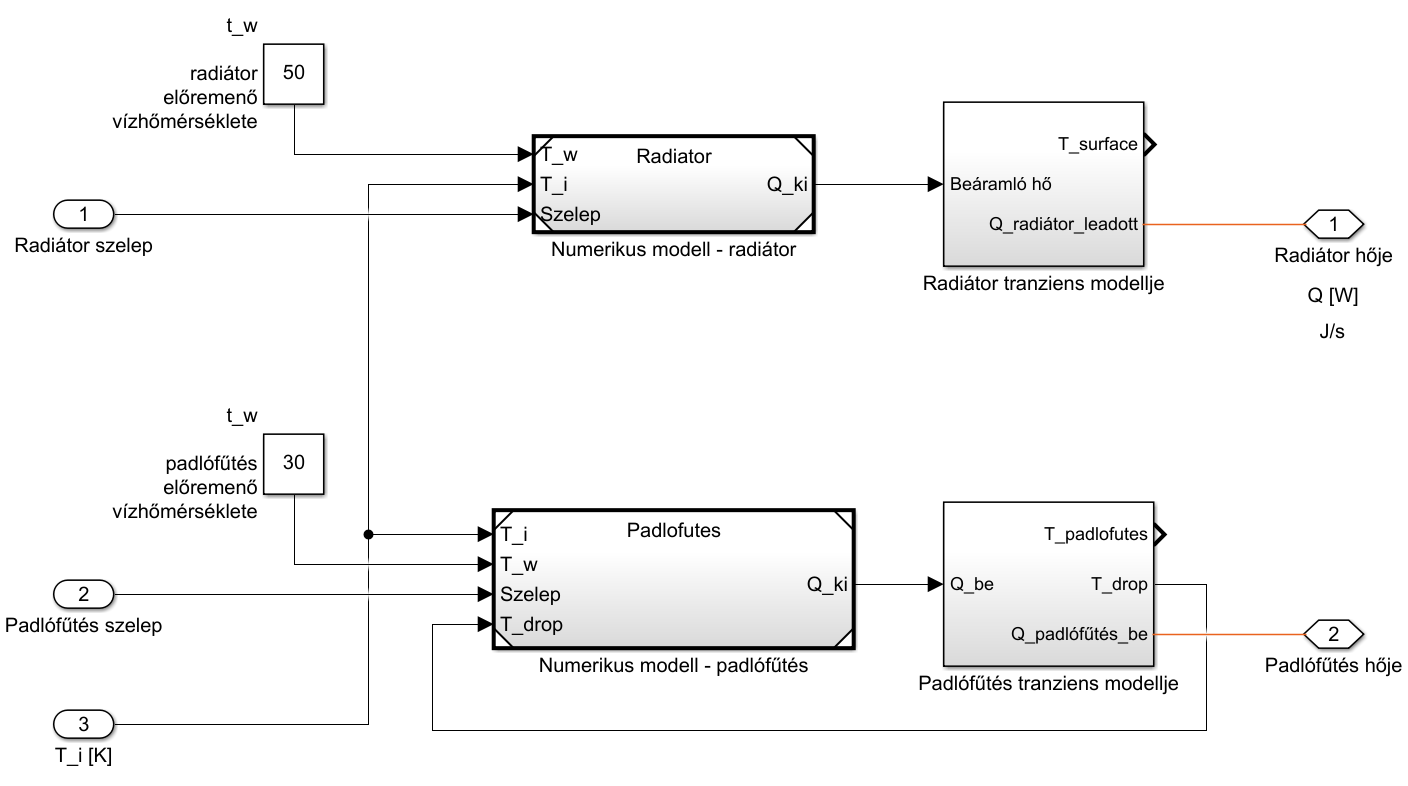
\includegraphics[trim=0 10 0 0, clip,width=0.9\textwidth]{figures/simscape/heatsys}
	\caption{Fűtőtestek modellje}
	\label{fig:SimscapeHeatSys}
\end{figure}



%Szimuláció során olyan bekapcsolási tranziensekkel is számolnom kell, amik egy kis időállandós fűtés (pl. légbefúvás, fan-coil) esetén elhanyagolhatók lennének.
%A modellalkotás során kétféle probléma merül fel. Egyrészt modellezni kell a fűtőtestek állandósult állapotbeli hőleadást. Másrészt, ha a fűtési rendszer időállandója nagy, akkor a tranziens lefolyása is lényeges a szabályzás szempontjából.
\section{Állandósult állapotbeli hőleadás numerikus modellje}\label{section:allandosult}

Mivel a vizsgált fűtési rendszerek hője melegvízből származik, a fűtővíz %kazán (hőszivattyú, stb.) által előállított melegvíz
hőmérséklete, illetve a keringető szivattyú tömegárama lehet a hőleadást befolyásoló paraméter\footnote{A kazánok a víz hőmérsékletét képesek változtatni időjárás függvényében, így az egy külön rendszer része lehet. Nem célom kazánvezérlést írni, az egyszerűség kedvéért feltételezem, hogy a melegvíz például távhő formában rendelkezésre áll.}. Az elképzelésemmel jobban összhangban áll az utóbbi választása, hiszen szelepekkel elosztottan, szobánként is szabályozható az egyes fűtőtestekbe táplált hőmennyiség: a víz tömegáramát folytonosan tudom szabályozni egy szelep segítségével\footnote{A \textit{\ref{chap:feasibility-tech}. fejezetben} mutatom be a megvalósíthatóság technikai feltételeit, például azt, hogy milyen szelep használatos erre a feladatra.}. A fűtőtestekbe betáplált víz hőmérséklete (úgynevezett előremenő hőmérséklet) állandó.

%\vspace{6pt}

A fűtőtest hőleadása függ a környezetétől is. A szabályzott jellemzőn felül a modell bemenetéhez tartozik a környezet hőmérséklete, ami a levegő vagy a fűtetlen objektumok hőmérséklete\footnote{A hőleadás típusa dönti el, hogy ezek közül melyik mérvadó. Különböző típusú fűtőtesteknél a teljesítmény más-más arányban oszlik meg konvektív és radiatív hőátadás között.}.
Ezen bemenő paraméterek és a fizikai tulajdonságok alapján megadható az állandósult állapotbeli teljesítmény. Ennek levezetése ebben a bekezdésben található.

A tranziensek a fűtőtestek fizikai kialakításától függnek. Minél nagyobb tömeget kell átmelegíteni azelőtt, hogy a fűtőtest felszínén a hőleadás megindulna, annál lassabb a beállási ideje az állandósult állapotnak. Kikapcsoláskor a fűtőtest a szelep elzárása után is ad le hőt. %Így egy adott referencia trajektória esetén figyelembe kell venni ezen rendszerek dinamikáját is.
A hőtárolási paramétereket könyvekből, publikációkból, gyártói katalógusokból, méréssel, vagy becsléssel határoztam meg. A Simscape-ben minden blokknak olyan fizikai tartalma van, amiben ezek a jellemzők bevihetők, hatásuk megfigyelhető. Ezt a modellt a \textit{\ref{section:dinamikus}. bekezdésben} láthatjuk.
%A modellhez szükség van pl. a fűtőtest felületi hőmérsékletének, vagy a visszatérő (lehűlt) víz hőmérsékletének mérésére.% A modellezéshez korlátozottan áll rendelkezésre információ, ugyanis nem 

%\textbf{\textit{TIKZPICTURE A MODELLRŐL, DIMENZIÓKRÓL}}

%\begin{figure}[h]
	\centering
	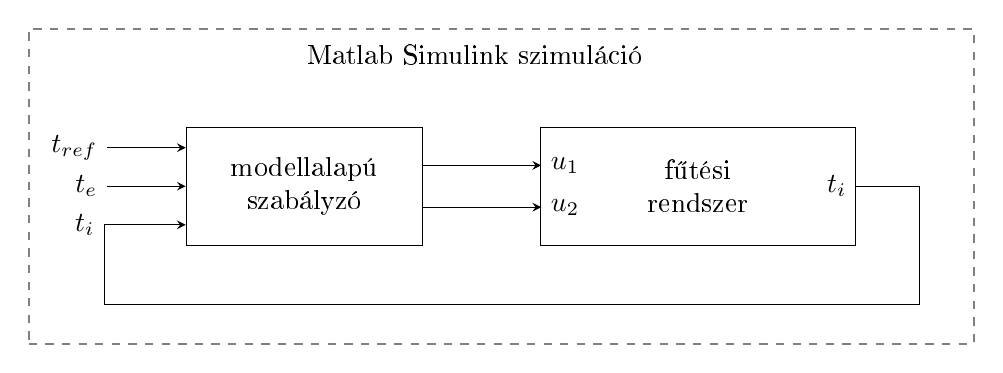
\begin{tikzpicture}[>=stealth,
	outer/.style={draw=gray,dashed,thick,inner sep=5pt}]

	% nagy blokkok
	\node[draw,rectangle, minimum height=1.5cm,minimum width=4cm] (plant) at (5,2.5) {\parbox{2cm}{\centering fűtési rendszer}};
	\node[draw,rectangle, minimum height=1.5cm,minimum width=3cm] (Control) at (0,2.5) {\parbox{2.5cm}{\centering modellalapú\\szabályzó}};
	
	% szaggatott vonal
	\node[draw,outer,rectangle, minimum height=4cm,minimum width=12cm,
	label={[label distance=-0.1cm, anchor=north]100:Matlab Simulink szimuláció}] (keret) at (2.5,2.5) {};
	
	
	% szabályzott mennyiségek
	\draw [->] (Control.10) node[right]{} -- +(15mm,0) node[right]{${u_{1}}$};
	\draw [->] (Control.350) node[right]{} -- +(15mm,0) node[right]{${u_{2}}$};
	
	%\draw[->] (Control.350) node[left]{} --  (plant.187) node[right]{${u_{2}}$};  %node[above left]{$\alpha_{radiator}$}; 
	%\draw[->] (Control.10) node[left]{} --  (plant.173) node[right]{${u_{1}}$} ;
	
	%\draw[->] (d.0) node[left]{heat [W]} ->  ++(3,0) ->  (house.180);
	
	
	% szabályzó bemenetei
	% a -| és |- máshogy fog törni, ha unconstraintelt.
	\draw [->] (plant.0)  node[left]{$t_i$} -|++(0.8,-1.5) -| ++(-9.25,0) |-  ++(-1.1,0) |- node[left]{$t_i$} (Control.198);
	
	%++(1.5cm,0) -- (2cm,0pt) -- (2.5cm,10pt);
	%\draw [->] (plant.0) node[left]{$t_i$ [\si{\celsius}]} -|++(1,0)|- -|++(-2.5,0)|- (Control.198) node[right]{}; %++(1.5cm,0) -- (2cm,0pt) -- (2.5cm,10pt);
	\draw [<-] (Control.180) node[right]{} -- +(-10mm,0) node[left]{$t_{e}$};
	\draw [<-] (Control.162) node[right]{} -- +(-10mm,0) node[left]{$t_{ref}$};
	
	%\draw[->] (House.180)  node[right]{${T_i}$} -| ++(-5.5,2)  |- (Control.180) ;
	%\draw[->] (d.20) -| ++(1,-1) |- (y.350);
	
	%\path 
	%(d.150)	 edge[<->] 	node[anchor=north,above]{valvePercent}	(y.270);
	
	\end{tikzpicture}

	\caption{A szimulációban szereplő elemek kapcsolata}
	\label{controlloop}
\end{figure}

%\begin{tikzpicture}[>=stealth,remember picture]
%\node[draw,rectangle,inner sep=0.5cm] (y) at (0,0) {$A$};
%\node[draw] (d) at (0,2) {%
%%	\begin{tikzpicture}[remember picture]
%%	\matrix [matrix of math nodes] (mat)
%%	{
%%		B & \phantom{C}   \\
%%		\phantom{B} & C \\
%%	};
%%	\end{tikzpicture}
%%};
%%\draw[->,shorten >= 6pt] (y.west) -| ++(-1,1) |- (mat-1-1);
%%\draw[->,shorten >= 6pt] (y.west) -| ++(-0.8,1) |- (mat-2-1);
%%\draw[->] ($(mat-2-2)+(14pt,0)$) -| ++(0.8,-1) |- (y.east);
%%\draw[->] ($(mat-1-2)+(14pt,0)$) -| ++(1,-1) |- (y.east);
%\end{tikzpicture}





\begin{formal}
%A munka elkezdésekor egy Simulink példa hálózatból indultam ki. Mivel a Matlab szimulációban a légbefúvásos fűtés modelljének teljesítmény kimenete van, olyan modellt szerettem volna felírni, ami beilleszthető az eredeti légbefúvó rendszer helyére. A ház hőveszteségeit a Matlab számolja\footnote{Pontosításra szorul ez a modell is, mert valószínűleg csak a konvektív hővezetéssel számol (a sugárzásival pedig nem). A légbefúvás a ház levegőjét melegíti. Ám a modellben a ház hőtároló tömege nem jelenik meg, csak egy hőellenállás a veszteségek modellezéséhez.}, ebből pedig adódik a szoba levegőjének hőmérséklete. A rendszer szabályozását így visszavezettem a leadott teljesítmény szabályzására. A levezetett egyenletnek köszönhetően egy teljesítményigényhez meg tudom majd mondani hogy mennyire kell a szabályzószelepeket kinyitni.
%
%Angol nyelvű szakirodalomból pl. Gouda2000 alapján számolva irreális teljesítményértékeket kaptam (150kW), tovább keresve magyar nyelvű irodalmat is áttekintettem.
%
%Az \textit{Épületgépészet a gyakorlatban}\footnote{Könyvtári könyv, Verlag. 5.11.6, 2. o.} c. könyvben szó esik fűtési rendszerek méretezéséről. Itt adatként szerepel egy épületre a szobák hőigénye\footnote{Pontosan nem tudom még, hogyan definiálják a hőigényt: mekkora kültéri hőmérsékletet vesznek pl. figyelembe, illetve hogy radiátor méretezésénél ezt nyilván felül kell becsülni.} és névleges hőmérséklete. Ehhez választanak megfelelő méretű radiátort, hogy azokban a kiszámolt sebességgel vizet keringetve a hőleadás elég legyen az adott helyiségbe.
%
%{\scriptsize(Ehhez figyelembe kell venni minden radiátorra a keringő víz hőmérsékletét is, különösen ha azok sorba vannak kötve és a hőmérsékletesések is jelentősek.)}
%
% Adottnak véve az előremenő és visszatérő hőmérsékletet az összes hőigényből számolható a víz kívánt áramlási sebessége. Ezután meghatározzák a radiátorok méretét, hogy azoknak a hőleadása megfeleljen az előírtaknak.
%
%A fenti példák segítenek a modellalkotásban is, felírható a radiátorok teljesítménye változó vízhőmérséklet és víz tömegáram esetén is. Természetesen a modell egyik bemenete, ez esetben a tömegáram a szabályzott mennyiség. Felteszem, hogy ezt folytonosan tudjuk szabályozni egy szelep segítségével (vagy ha ez nem életszerű, akkor kétállású szeleppel, de nagyobb frekvenciával, mint ahogy egy kazánt tudnánk ki/be kapcsolni).
\textbf{Megjegyzés:} A méretezési feladatot \textit{Csoknyai} \cite[359.~o.]{Herz} tárgyalja. Ezek alapján vezettem le a leadott hő mennyiségét állandósult állapotra. Természetesen a felmelegedés és lehűlés idejét is figyelembe kell majd venni, de ezzel érthető módon a méretezésnél nem számolnak.

%További egyszerűsítésként elhanyagoltam a hőleadási tényező hőmérsékletfüggését is.
%Itt a hőveszteség adott. Esetünkben ezt a házra a Matlab számolja és jól méretezett rendszert tételezünk fel. Csupán azért kell a hőleadást jól felírni, hogy a felfutás, hőkapacitás, stb. során átadott energiát is belekalkuláljuk.
\end{formal}
%Persze ilyenkor egyedi esetekből indulok ki, de remélhetőleg ez paraméterezhetően elvezet az általános, többféle házra alkalmazható megoldáshoz.

%\subsection*{Nomenklatúra} az elejére.

\subsection{Hőleadás alapegyenletei}
A fűtőtestek hőleadása az alábbi alakban írható (\textit{Csoknyai} \cite[358.~o.]{Herz}):
%(A 86. oldalon $\Delta t_k$, a 358.-on $\Delta t_m$ jelöléssel találkozunk. A \cite[359.~o.]{Herz} ismét változik ugyanannak a jelölése. (\ref{termeszeteshk_359}) Ezutóbbi angol jelölés szimpatikusabb.)
\begin{equation} \label{eq_holeadas}
 Q_{le} = h_t ~ A_e ~ (t_{surf} - t_i)
\end{equation}
ahol
\begin{itemize}[itemsep=6pt,topsep=0pt,parsep=0pt,partopsep=0pt]
\item[] ${Q}_{le}$ [\SI{}{\watt}] a leadott hő
\item[] $h_t$ [\si[per-mode = fraction]{\watt\per\meter\squared\per\kelvin}] a teljes hőleadási tényező %- ezt hőmérsékletfüggetlennek tekintem.
\item[] $A_e$ [\si{\metre\squared}] a radiátor felülete
\item[] $t_{surf}$ a fűtőtest felületi hőmérséklete\footnote{A felületi hőmérsékletet nem tudjuk közvetlenül mérni, ezért ki kell fejeznünk ismert jellemzőkkel.}
%\item[] $\Delta t_m$ [\SI{}{\kelvin}] a közepes hőmérsékletkülönbség:
\end{itemize}
\begin{equation} \label{eq_termeszeteshk_359}
\begin{aligned}
t_{surf} = \frac{t_w+t_r}{2} -t_{drop}
\end{aligned}
\end{equation}
ahol \si{\celsius}-ban szerepelnek:
\begin{itemize}[itemsep=6pt,topsep=0pt,parsep=0pt,partopsep=0pt]
	\item[] $t_i$ a szoba hőmérséklete
	\item[] $t_w$ a radiátorba befolyó, $t_r$ az onnan kifolyó víz hőmérséklete, ebből $\frac{t_w+t_r}{2}$ az átlagos vízhőmérséklet
	\item[] $t_{drop}$ hőmérsékletesés a közepes fűtővízhőmérséklethez képest\footnote{A hőleadás során a fűtőközeg és a fűtőtest felülete közötti konduktív hővezetés miatt hőmérsékletesés lép fel. A padlófűtésnél lesz ez különösen releváns, hiszen ott a felület hőmérséklete jóval alacsonyabb, mint a be- és kimenő vízhőmérsékletek átlaga: hiába fűtünk \SI{40}{\celsius}-os vízzel, a padló kb. \SI{25}{\celsius}-os lesz.}
\end{itemize}
%A hőátadási tényező is hőmérsékletfüggő, de ezzel egyelőre nem foglalkozom, állandónak tekintem.
%\begin{equation} \label{k_e}
%k_e = \frac{\dot{Q}}{A~ \Delta t_m}
%\end{equation}
%
%A hőteljesítmény hőmérsékletfüggő (361.~o.). Az $x^{1.33}$ az egyenletekben $x~ x^{1/3}$, ebből pedig $ x ~ \sqrt[3]{x}$ formában jelenik meg.
%
%
%Nominálisan $\Delta t_m$ = \SI{60}{\celsius}-ra adott érték a közepes hőmérsékletkülönbség függvényében változik:
%
\subsection{Hőfelvétel alapegyenletei}
A vízből felvett hő felírható:
\begin{equation} \label{eq_hofelvetel}
 Q_{fel} = c ~ (u\dot{m}_0) ~ \Delta t=c ~ \dot{m} ~ \Delta t
\end{equation}
ahol
\begin{itemize}[itemsep=6pt,topsep=0pt,parsep=0pt,partopsep=0pt]
	\item[] ${Q}_{fel}$ [\SI{}{\watt}] a vízből felvett hő, ami annak lehűléséből adódik
	\item[] $c$ [\si[per-mode = fraction]{\joule\per\kg\per\kelvin}] a víz fajhője
	\item[] $u$ a szabályzó beavatkozó jele, $ u \in [0,1]$ folytonosan változhat 0 és 1 között
	\item[] $\dot{m}_0$ [\si[per-mode = fraction]{\kg\per\second}] a víz maximális tömegárama, $\dot{m}$ a szabályozott tömegáram.
	\item[] $\Delta t = t_w-t_r$ [\SI{}{\kelvin}] a víz lehűlésének mértéke
\end{itemize}

\subsection{Energiamérleg állandósult állapotban}
\textbf{Állandósult állapot} esetén a leadott hő egyenlő a felvettel, mivel akkor nem történik hőfelhalmozás, hőtárolás.
Azaz ekkor a radiátor hőkapacitását nem kell figyelembe vennem.

Beírva a (\ref{eq_holeadas})-be (\ref{eq_termeszeteshk_359})-t:
\begin{equation} \label{eq_holeadas2}
\begin{aligned}
 Q_{le} = h_t ~ A_e ~ \left( \frac{t_w+t_r}{2}-t_{drop} - t_i\right) = h_t ~ A_e ~ \left( \frac{t_w+(t_w-\Delta t)}{2}-t_{drop}-t_i\right)
\end{aligned}
\end{equation}

Ahol felhasználtuk azt is, hogy $t_r = t_w-\Delta t$, majd $\Delta t$ helyére beírhatjuk a (\ref{eq_hofelvetel})  átrendezett alakját:
\begin{equation} \label{eq_hofelvetel2}
~~\Delta t = \frac{ Q_{fel}}{c ~ \dot{m}}
\end{equation}

Beírva (\ref{eq_holeadas2})-ba (\ref{eq_hofelvetel2})-t:
\begin{equation} \label{holeadas3}
\begin{aligned}
 Q_{le} ~=~ & h_t~ A_e\left( t_w-\frac{ Q_{fel}}{2~c ~ \dot{m}}-t_{drop}-t_i\right)  \\[18pt]
%\Delta t_m &\triangleq  t_w-t_i-\frac{\dot Q_{fel}}{2~c ~ \dot{m}}
%\\[18pt]
 Q_{le} + \frac{h_t ~ A_e ~  Q_{fel}}{2 ~ c ~ \dot{m}} ~ = ~ & h_t ~ A_e ~\left( t_w-t_{drop}-t_i\right) \\[24pt]
2 ~ c ~ \dot{m} ~  Q_{le} + h_t ~ A_e ~  Q_{fel} ~ = ~ &  h_t ~ A_e ~ 2~ c~ \dot{m} ~\left( t_w-t_{drop}-t_i\right)
\end{aligned}
\end{equation}

\textbf{Csak abban az esetben, ha} $ Q_{le}= Q_{fel}$:

%(meggondolandó hogy a hőkapacitások szerepe hogy alakul...)


\begin{equation} \label{eq_holeadas4}
\begin{aligned}
~~~~~~ Q (2 ~ c ~ \dot{m} + h_t ~ A_e) & ~=~ 2 ~ h_t ~ A_e ~ c~ \dot{m} ~(t_w-t_{drop}-t_i) \\[18pt]
~~~~~~ Q &~=~ \frac{2~c~\dot{m}~h_t~A_e}{2 ~c ~ \dot{m} + h_t ~ A_e}~(t_w-t_{drop}-t_i)
\end{aligned}
\end{equation}

Ez adja meg a fűtési rendszer által szolgáltatott teljesítményt állandósult állapotban.
A fenti képletben a hőleadási tényezőt hőmérsékletfüggőnek is lehet venni, \textit{Cholewa}~\cite{CHOLEWA2013599} mérései alapján.

Állandósult állapotra a szükséges beavatkozójel adott kimenő teljesítményhez a \ref{eq_holeadas4} egyenletet kell $\dot{m}$-ra rendezni, a beavatkozó jel $u=\dot{m}/\dot{m}_0$.

Mivel a hőleadást, hőtárolást Simscape-ben valósítottam meg, a radiátorba bemenő hőt kell csak kiszámítani. Erre meg kell vizsgálni, hogy az állandósult állapotbeli képlet helyes-e.



\section{Hőátadás tranziensének modellje}\label{section:dinamikus}

% \subsubsection*{Nomenklatúra}

A különböző hőtároló elemek feltöltődése szimulálva adja a dinamikus viselkedést. A Simscape hálózatok és azok paraméterei az egyes fűtőtesteknél találhatók.

Katalógusból radiátorok tömege és a bennük lévő víz térfogata leolvasható. A hőkapacitás számítása:

\begin{equation} \label{eq_hotartalom}
C = c_{m} ~ m_m ~ \Delta t_k + c_{w} ~ m_w ~ \Delta t_k
\end{equation}

Ahol m a material, azaz a fűtőtest anyagára utal, $m_w$ pedig a víz mennyiségére. A hőmennyiség joule-ban adott.


%\subsection{Hőleadás hőmérsékletfüggése}




%\newpage

%Fun facts:
%~
%\begin{itemize}[itemsep=6pt,topsep=0pt,parsep=0pt,partopsep=0pt]
%	\item A falakra az $\alpha$ = 10 \si[per-mode = fraction]{\watt\per\meter\squared\per\kelvin} érték a sugárzó és konvektív hőleadást is tartalmazza. A konvektív hőleadás függ a felületi áramlási sebességtől: falsaroknál ez az érték alacsonyabb, kb. a fele.
%	\item A sugárzó hő a Stefan-Boltzmann törvény alapján függ az emisszivitástól. (Annak a mértéke, hogy a test a feketetesthez képest mennyi hőt bocsát ki). A hőmennyiség a hőmérséklet negyedik hatványával arányos. A \textbf{sugárzott hő meghatározásához} még meg kell keresni és be kell írni a Simscape blokkba a megfelelő együtthatókat. Valami általános összefüggést kell találni, hogy a radiátor milyen arányban melegíti a külső falat, ahol van, ill. az ablakra milyen hatással van: még nem kezelem le ezeket az aszimmetriákat, hanem minden hőmérsékleteloszlást homogénnek veszek. A Stefan-Boltzmann törvény direkt alkalmazása helyett a szabványokban és irodalomban található közelítésekkel élek.
%	
%%	\item A $q_r$ [\si[per-mode = fraction]{\watt\per\meter\squared}] \textit{radiant heat flux density} a \cite{CHOLEWA2013599} T. Cholewa
%%	%\footnote{On the heat transfer coefficients between heated/cooled radiant floor and room. \\ DOI: http://dx.doi.org/10.1016/j.enbuild.2013.07.065}
%%	(5.) egyenlet alapján számítható de az a geometriától is nagyban függ. Helyette Kilkis1994 (4) és (6) javasolt, illetve a \cite{CHOLEWA2013599}-ból is lehet mért értékekkel számolni / a szabványok ajánlását használni.
%
%
%	\item A hőhidak a hőveszteségek meglepően nagy részéért felelősek, jelentős hibát követünk el, ha ezekkel nem számolunk. Az energetikai tanúsítvány számol ezekkel, így a modellben a veszteséghez ezt is hozzá lehet adni.
%	
%	
%	\item \cite[5.188.~o.]{watson2002radiant} szerint az operatív hőmérséklet $t_{op}~=~\frac{h_rT_{mrt}~+~h_cT_{air}}{h_{tot}}$, ahol $T_{mrt}~=~\frac{\sum\limits_{k=1}^{n}A_k\epsilon_kT_k}{\sum\limits_{k=1}^{n}A_k\epsilon_k}$. Az $\epsilon$ emittancia a StefBol képletből való.
%	
%	
%\end{itemize} 
%
%Fűtött padló, falak, mennyezet esetén jelentős szerepe van a sugárzó hőleadásnak.
%
%\begin{itemize}[itemsep=0pt,topsep=0pt,parsep=0pt,partopsep=0pt]
%	\item A.Laouadi / Building and Environment 39 (2004) 421 – 431 - p424, eq. 10-11: radiant heat transfer model - (11)-es egyenlet
%	\item TEMPERATURE CONTROL STRATEGIES FOR RADIANT FLOOR HEATING SYSTEMS, Zhi Long Zhang: 40.o.  
%%	\item \cite{CHOLEWA2013599} T. Cholewa et al. / Energy and Buildings 66 (2013) 599–606 - Table 5: coefficient
%%	\item Kilkis1994 A simplified model for radiant heating and cooling panels: itt van képlet sugárzóra
%	\item Kiegészítés: \cite[349.~o.]{Herz}
%\end{itemize}  

\section{Radiátor modellje}

\textit{\ref{eq_holeadas4}. egyenletben} szereplő paraméterek értéke az állandósult állapotbeli hőleadáshoz:

\begin{table}[H]
	\footnotesize
	\centering

	%\renewcommand{\arraystretch}{2} % to increase cell height
	%\taburulecolor{gray}
	%\begin{tabular}{|p{0.8cm}|p{1cm}|p{1cm}|p{1cm}|p{1cm}|p{1cm}|p{1cm}|p{1cm}|}
	%
	%\begin{tabulary}{\linewidth}{LLc}
	\begin{tabu}{@{}lll@{}}
		\hline
		$\dot{m}_0$ 	& maximális tömegáram 	& 0.05 \si[per-mode=symbol]{\kilogram\per\second}
		\\
		$h_t $		& hőátadási tényező		& 7 \si[per-mode=symbol]{\watt\per\metre\squared\per\kelvin}
		\\
		$A $		& felszín				& 4 \si[per-mode=symbol]{\metre\squared}
		\\
		$t_{drop}$ 	& hőmérsékletesés 		& 0 \si[per-mode=symbol]{\celsius}
		\\ \hline
	\end{tabu}
	\label{tab:RadiatorDetail}
	\caption{Radiátor adatai állandósult állapotbeli számításokhoz}
	%\label{tab:TabularExample}
	%\tabref{TabularExample}~táblázat
\end{table}

Ahol a $t_{drop}$=0 közelítés azért megengedhető, mert a fémtesten kicsi a hőmérsékletesés, így az átlagos felületi hőmérséklet közel azonos az átlagos vízhőmérséklettel. A tranziensben a két hőtároló tömeg a pontosabb szimuláció miatt szerepel külön.

A tranzienseket a Simscape hálózat adja:

\begin{figure}[H]
	\centering
	% trim={<left> <lower> <right> <upper>}
	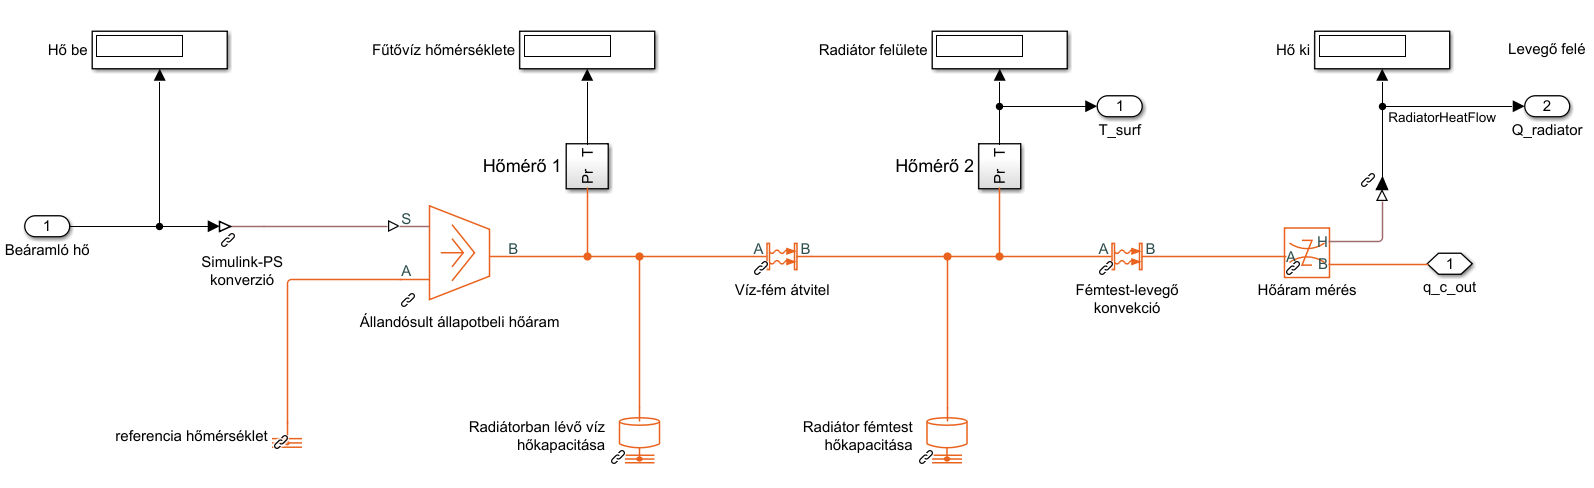
\includegraphics[trim=0 0 0 0, clip,width=\textwidth]{figures/simscape/radiator}
	\caption{Radiátor Simscape modellje}
	\label{fig:SimscapeRadiator}
\end{figure}

A felmelegedéskor és lehűléskor a pontos hőleadást akkor tudjuk modellezni, ha ismerjük a radiátor hőkapacitását. Ehhez tudnunk kell, hogy a radiátorban mennyi víz van, illetve hogy a radiátortest milyen nehéz.
A radiátorokat mindig az adott helyiséghez méretezik, ezért az adatokat leolvasással vagy katalógusból kapjuk normál esetben. A modellezéshez választanom kellett egy típust. Itt még csak paraméteresen kellene megadni az értékeket, vagy előbb a ház modelljét, hőszükségletét felírni, hiszen a házhoz tervezzük a fűtést és nem fordítva.

Radiátor katalógusokból azt találtam, hogy az egyes radiátor típusokra ezek a paraméterek milyen értékűek. Itt a teljesítményt is feltüntetik, így a megfelelőt tudtam kiválasztani.

A termikus modell paraméterei egy 90 cm magas, 1,8 m hosszú C22 típusú radiátorra\footnote{Purmo Ventil Compact - purmo.com/hu/termekek/lapradiatorok/purmo-ventil-compact.htm} az alábbi táblázatban találhatóak:

\begin{table}[H]
	\footnotesize
	\centering

	%\renewcommand{\arraystretch}{2} % to increase cell height
	%\taburulecolor{gray}
	%\begin{tabular}{|p{0.8cm}|p{1cm}|p{1cm}|p{1cm}|p{1cm}|p{1cm}|p{1cm}|p{1cm}|}
	%
	%\begin{tabulary}{\linewidth}{LLc}
	\begin{tabu}{@{}ll@{}}
		\hline
		fémtest tömege 	& 90 \si[per-mode=symbol]{\kilogram}
		\\
		fémtest fajhője	& 464 \si[per-mode=symbol]{\joule\per\kilogram\per\kelvin}
		\\
		fűtővíz tömege	& 16 \si[per-mode=symbol]{\kilogram}
		\\
		víz fajhője		& 4189 \si[per-mode=symbol]{\joule\per\kilogram\per\kelvin}
		\\ \hline
	\end{tabu}
	\label{tab:RadiatorHeatCap}
	\caption{Radiátor adatai a tranziensekhez}
	%\label{tab:TabularExample}
	%\tabref{TabularExample}~táblázat
\end{table}

% \begin{table}[H]
	\centering
	
	\renewcommand{\arraystretch}{2} % to increase cell height
	\taburulecolor{gray}
	
	%\begin{tabular}{|p{0.8cm}|p{1cm}|p{1cm}|p{1cm}|p{1cm}|p{1cm}|p{1cm}|p{1cm}|}
	
	\newcolumntype{C}[1]{>{\centering\arraybackslash}p{#1}}
	\newcolumntype{R}[1]{>{\raggedleft\arraybackslash}p{#1}}
	
	\begin{tabu}{p{2.5cm}p{3cm}p{3cm}p{2.8cm}c}
		%\cline{2-5}
		\multicolumn{1}{l}{} 	& Komponens & Hőleadás & Hőtároló tömeg & Fajhő \\ %\cline{2-5}
%		\multicolumn{5}{c}{}\\ %\hline
		% header
%		\multirow{2}{*}
%		{Radiátor} & \multicolumn{2}{c|}{Time} \\	\cline{2-3}
%		& First flight & Second flight\\ 

		\hline
		\multirow{2}{*}
					{Radiátor} 	 & víz 		& a fémtestnek	& 8.9 \si[per-mode=symbol]{\kilogram\per\metre} 	& 4189 \si[per-mode=symbol]{\joule\per\kilogram\per\kelvin}	\\ % \cline{2-5}
								 & fémtest 	& a levegőnek	& 50.1 \si[per-mode=symbol]{\kilogram\per\metre}	& 464 \si[per-mode=symbol]{\joule\per\kilogram\per\kelvin}	\\  %\hline
								 
		\hline
		
		\multirow{3}{*}
					{Padlófűtés} & Padló betonja 	& hővezetés	& 840  \si[per-mode=fraction]{\kilogram\per\metre\squared}	&	\\  %\cline{2-5}
								 & Padló burkolat 	& hővezetés 	&	& 	\\  \hline
	\end{tabu}						
		% entries - event names aligned left with multicolumn
%		\multicolumn{1}{|l|}{flightHAT turned on} 	& & \\ \hline
%%		{|p{3cm}|p{1cm}|p{3cm}|p{3cm}|p{3cm}|}
%		%{p{1.5cm}|C{0.8cm}|C{0.8cm}|C{0.8cm}|C{0.8cm}|C{0.8cm}|C{0.8cm}|C{0.8cm}|C{0.8cm}|}
%		%\multicolumn{1}{l}{}&\multicolumn{8}{l}{SDO header (első adatbyte) - master kérése}
%		%\\ 		\cline{2-9}\cline{2-9}
%		\hline
%		felület& méret & kalorikus hőátbocsátási tényező    & hőtároló tömeg & hőkapac
%		
%		\\ \hline
%		külső fal & 4.5 \si{\metre\squared} & 2 \si[per-mode=fraction]{\watt\per\metre\squared\per\kelvin} & 4.5*200kg & e.g. 4.5*200*840 \si[per-mode=fraction]{\joule\per\kelvin}
%		\\ \hline
%		ablak & 4 \si{\metre\squared} & 4 \si[per-mode=fraction]{\watt\per\metre\squared\per\kelvin} & 0 & 0
%		\\ \hline
%		belső válaszfalak & 50 \si{\metre\squared} & 7 & 50*100kg & 50*100*840	
%		\\ \hline
%		padló & 16 \si{\metre\squared} & 11 & 16*200kg & 169*200*840	
%		\\ \hline
%		mennyezet & 16 \si{\metre\squared} & ? rad / conv &  & 	
%%		\\ \hline

	
	\caption{Fűtőtestek termikus tulajdonságai}
	\label{table_heater_parameters}
\end{table}
 helzett

A radiátor hossza, magassága, konstrukciója alapján a tömegek kiszámíthatók, illetve az acél hőkapacitása katalógusadatként szerepel.
A szimulációban a  Simscape termikus hőtároló elem blokkjaiba a fenti adatokat írtam.%, a víz fajhője még egy hőtároló elem.


\section{Padlófűtés modellje}

A padlófűtések felépítése az alábbi ábrán található. Egy hőszigetelő rétegre kerülnek a műanyag csövek, bizonyos elrendezésben. Erre híg betont öntenek, hogy az a csövek teljes felületét körbevegye, ne alakuljanak ki zárványok. Ha a beton nem veszi teljesen körbe a fűtéscsöveket, a padlófűtés teljesítménye lecsökken. A beton hőellenállása nem hanyagolható el, ezért a szimulációban ezt a hőmérsékletesést is figyelembe veszem. A hőszigetelő réteg biztosítja, hogy a hő a felső rétegek felé terjedjen.

\begin{figure}[H]
	\centering
	% trim={<left> <lower> <right> <upper>}
	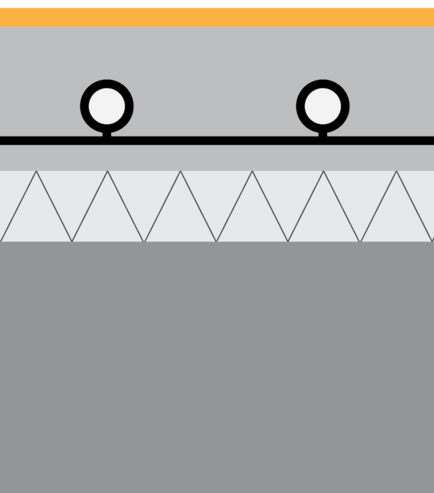
\includegraphics[trim=0 70 0 0, clip,width=0.25\textwidth]{figures/ISO11855typeA}
	\caption{A-típusú padlószerkezet (EN1264) fűtéscsővel}
	\label{fig:futotest-padlofutes}
\end{figure}

\textit{Olesen} számításait\footnote{A számítások Olesen kurzusának anyagában találhatók. \\
	\url{https://www.iee-cense.eu/-/media/Sites/Iee-cense/information/information-for-teachers/lecture-,-d-,2/presentation-slides/lecture_2c_dimensioning.ashx}} használtam a méretezéshez.
A \SI{18}{\metre\squared} alapterületű helyiségben \SI{15}{\metre\squared}-nek vettem a fűtött területet. Ebből, és a hőigényből 45\si[per-mode=symbol]{\watt\per\metre\squared} teljesítményigény adódott.
Az előremenő vízhőmérséklet kiszámítva $t_w =$\SI{36}{\celsius} biztosan fedezi a hőigényt $\dot{m}=$\SI{0.05}{\kilogram\per\second} tömegáram mellett.

\textit{Cholewa} \cite{CHOLEWA2013599} és \textit{Koca} \cite{Koca} falfűtés és mennyezetfűtés esetére mért $h_r$ és $h_c$ sugárzó és konvektív hőátadási tényezőket. Ezen mérési eredmények paramétereit helyettesítettem be a hőleadás egyenletébe ahhoz hogy eldöntsem, helytálló-e a felírt modell. Az említett publikációkban minden adat rendelkezésre áll. A következő eseteket vizsgáltam:

\begin{table}[H]
	\vspace{12pt}
	\centering
	\renewcommand{\arraystretch}{1.1} % to increase cell height..
	\begin{tabular}{
			l
			S[table-format=-3.2]
			S[table-format=-3.2]
			S[table-format=-3.2]
			S[table-format=-3.2]
			S[table-format=-3.2]
			%cccc
		}
		%\hline
		\multicolumn{1}{c}{Paraméter} & \multicolumn{5}{c}{Cholewa mérései}\\%& \multicolumn{1}{c}{dummy} \\
		\hline%\cline{1-2}
		%	$T_{water}$    & Description & Price & (\$) \\
		%	\hline
		$T_{water},\si{\celsius}$      								& 30	& 30	& 40	& 50	& 55   		\\
		%$\dot{m}$ [\si[per-mode=fraction]{\kilogram\per\second}]  	& 0.0167& 0.055	& 0.0167& 0.0167& 0.055    	\\
		$\dot{m}$ [\si[per-mode=symbol]{\kilogram\per\minute}]  	& 1		& 3		& 1		& 1		& 3		    \\
		$T_{surf}$													& 25.3	& 26.2	& 32    & 37.4  & 42.4		\\
		$T_{a0.6}$       											& 22.3  & 23.3 	& 26.9	& 30.8  & 34.3 		\\
		$h_{total0.6}$ [\si[per-mode=symbol]{\watt\per\metre\squared\per\kelvin}] 
		%\small{$\left[ \frac{\si{\watt}}{\si{\metre\squared\kelvin}} \right]$ }
		& 8.7   & 9.4  	& 9.7  	& 10.5  & 10.8  	\\[5pt] \hline 
		%$\Delta T$       											& 3     & 2.9	& 5.1  	& 6.6   & 8.1 		\\[5pt] \hline 
		$q_{total}$ [\si[per-mode=symbol]{\watt\per\metre\squared}]
		%\small{$\left[ \frac{\si{\watt}}{\si{\metre\squared}} \right]$}
		& 25.1  & 26.4  & 47.8  &  68.8	& 88.4   	\\[5pt] 		
		$q_{formula}$ [\si[per-mode=symbol]{\watt\per\metre\squared}]
		& 24.6  & 26.7  & 46.3  &  64.5 & 85.5   	\\[5pt] %\hline 
		Pontosság [\%]
		& 98	& 101	&  97	& 93.75 & 96.7		\\ %\hline
		\hline
	\end{tabular}
	\caption{A \ref{eq_holeadas4}. képlettel kapott eredmények és a \cite{CHOLEWA2013599} és \cite{Koca} eredményeinek összevetése}
	
\end{table}


% Az 1.1 méréseket használva rendre 10%-kal alábecsültük a hőt.
{\Large }


A hőleadás egyenletével számolt és a fent hivatkozott, méréssel kapott eredmények elég jól követik egymást. Padlófűtésnél a padló felületi hőmérséklettel számoltam, ugyanis a padló hőmérséklete jóval alacsonyabb, mint a fűtővíz hőmérséklete. A Simulink modell is figyelembe veszi a kb. 5 cm-s betonréteg $\lambda=$\SI{1.25}{\watt\per\metre} hővezetési ellenállását, a \textit{REHVA Guidebook \cite{RehvaGuidebookNo7}} szerint.
A fenti publikációkban figyelembe vették a hőleadási tényező hőmérsékletfüggését.\footnote{Intuitívan is belátható, hogy melegebb testnek nagyobb a konvektív hőleadási tényezője. A konvektív hőátadás mértéke nagyban függ attól, hogy a felületen milyen sebességgel áramlik a levegő, hiszen a forró tea gyorsabban hűl, ha fújjuk, illetve szélben a kinti hőmérséklet kisebbnek érződik. Hasonlóan melegebb tárgy esetén a légáramlás felgyorsul, amiatt hogy a melegebb levegő felfelé száll.} %Nagyobb felületi légáramlás tehát megnövekedett konvektív hőátadást eredményez.}
Azaz a felfutási tranziens során is változik a hőátadási tényező.

\begin{figure}[H]
	\centering
	% trim={<left> <lower> <right> <upper>}
	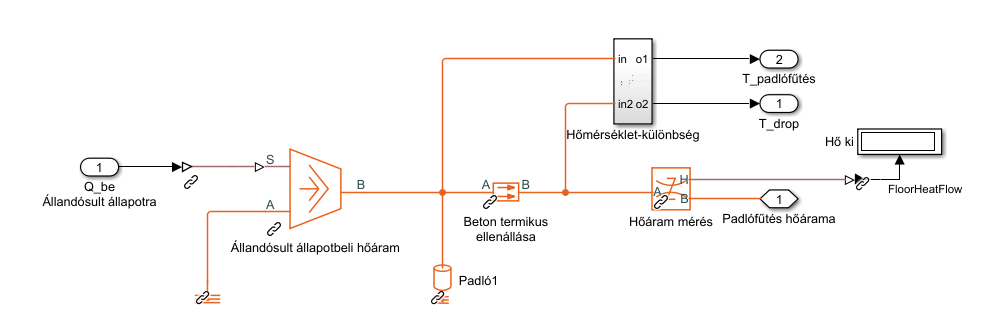
\includegraphics[trim=0 0 0 0, clip,width=\textwidth]{figures/simscape/padlo}
	\caption{Padlófűtés Simscape modellje}
	\label{fig:SimscapePadlo}
\end{figure}


\pagebreak
%\chapter{Modellek tesztje}
%
%\subsection{Radiátor unit test}
%
%\subsubsection{Állandósult állapot numerikus modellje}
%
%Annak ellenőrzése, hogy a \ref{holeadas4} egyenlet jó-e. Azaz elfogadható-e ez a közelítés állandósult állapotban, illetve a tranziens alatt mennyire feasible. 
%
%Az egyenletben a mintavételi idő egy szorzóként jelenik meg, 
%
%Az egyenlet wattban adja a kimenetét.
%A teszt egy formája lehet, ha a gyári adatokat (fűtési teljesítmény) összevetem az általam számoltakkal.
%
%\subsubsection{Tranziens Simscape modellje}
%A bejövő hő függvényében a hőleadás tranziensei. A bejövő hőt a képlet numerikusan számítja. A tranzienst viszont Simscape-ben szimulálom. Ez folytonos rendszert feltételez.
%
%\subsubsection{Szabályzás célja}
%
%Állandósult állapotban olyan bemenő hőáramot elérni, ami épp fedezi a veszteségeket.
%
%\subsection{Padlófűtés unit test}

\chapter{Identifikáció}\label{chap:ident}


A szabályzó tervezésénél használt szakaszmodell a Simulinkben megvalósított fizikai modell viselkedését leíró lineáris rendszer. Ebben a fejezetben a korábbiakban ismertetett hálózatot identifikálom.
\begin{figure}[h]
	\centering
	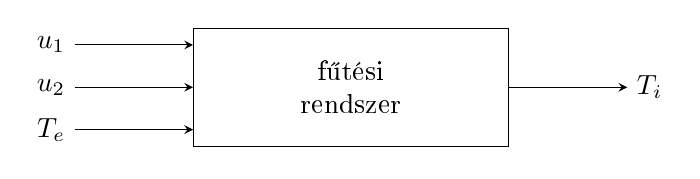
\begin{tikzpicture}[>=stealth,
outer/.style={draw=gray,dashed,thick,inner sep=5pt}]

% nagy blokkok
\node[draw,rectangle, minimum height=1.5cm,minimum width=4cm] (plant) at (0,2.5) {\parbox{2cm}{\centering fűtési rendszer}};
%\node[draw,rectangle, minimum height=1.5cm,minimum width=3cm] (Control) at (0,2.5) {\parbox{2.5cm}{\centering modellalapú\\szabályzó}};

% szaggatott vonal
%\node[draw,outer,rectangle, minimum height=4cm,minimum width=12cm,
%label={[label distance=-0.1cm, anchor=north]100:Matlab Simulink szimuláció}] (keret) at (2.5,2.5) {};


% plant bemenetei
\draw [<-] (plant.165) node[left]{} -- +(-15mm,0) node[left]{$u_{1}$};
\draw [<-] (plant.180) node[left]{} -- +(-15mm,0) node[left]{$u_{2}$};
\draw [<-] (plant.195) node[left]{} -- +(-15mm,0) node[left]{$T_{e}$};
\draw [->] (plant.0)   node[left]{} -- +(15mm,0) node[right]{$T_{i}$};

% szabályzó bemenetei
% a -| és |- máshogy fog törni, ha unconstraintelt.
%\draw [->] (plant.0)  node[left]{$t_i$} -|++(0.8,-1.5) -| ++(-9.25,0) |-  ++(-1.1,0) |- node[left]{$t_i$} (Control.198);

%\draw [<-] (Control.180) node[right]{} -- +(-10mm,0) node[left]{$t_{e}$};
%\draw [<-] (Control.162) node[right]{} -- +(-10mm,0) node[left]{$t_{ref}$};
\end{tikzpicture}
	\caption{A szabályzott szakasz összevont modellje}
	\label{tikz:simulation}
\end{figure}

A Simulinkben vizsgálójeleket használok: a több bemenetű, egy kimenetű rendszert egyszerre csak egy bemenetén gerjesztem. A tömegáramot szabályzó szelepek nyitott és csukott állapot között folytonosan állíthatók, 0 és 1 közötti beavatkozó jellel. A külső hőmérsékletet a modell kelvinben kapja, kimenete a belső hőmérséklet.

A szelepekkel való beavatkozás hiányában a $T_i$ belső és $T_e$ külső hőmérséklet különbsége (a helyiség időállandójának megfelelően) kiegyenlítődik.

 %(\textit{\ref{fig:valve-step}. ábra}). 
% a kimeneti változást létrehozó hatás egyértelműen beazonosítható kell hogy legyen.

\section{A szakasz ugrásválasza}

Lineáris hálózatoknál gyakori vizsgálójel az egységugrás, illetve az impulzusgerjesztés. Az identifikációhoz ugrásválaszt vizsgáltam, de mivel a rendszernek 3 bemenete van, ezekre nem egyszerre, hanem időben eltolva adtam ugrásgerjesztést, mindig megvárva, hogy az előző hatás tranziense lecsengjen. A következőkben viszont nem csak a tranziensek a fontosak, hanem a végértékek is. A következő három ábrán összevethetők a szakasz tulajdonságai egyes gerjesztésekre.

\begin{figure}[H]
	\centering
	% trim={<left> <lower> <right> <upper>}
	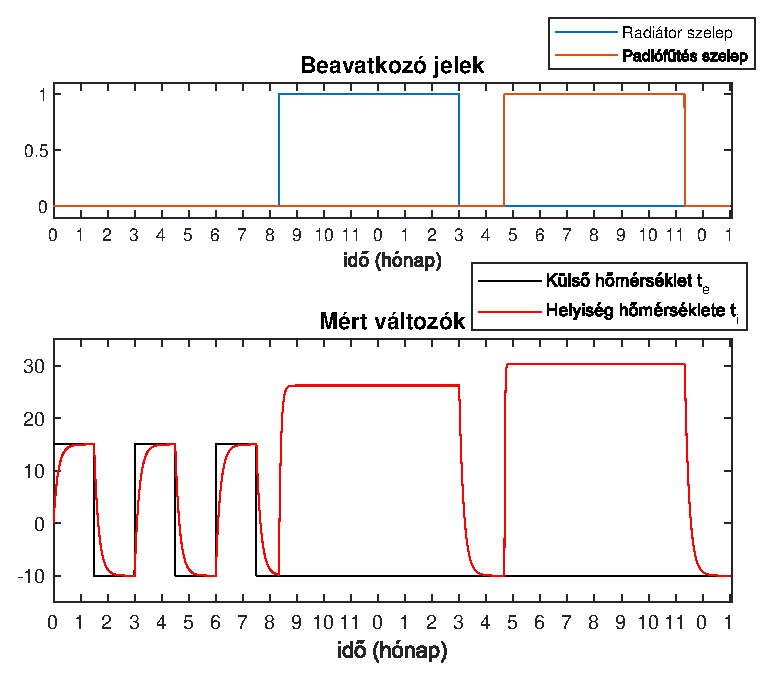
\includegraphics[trim=0 0 0 0, clip,width=0.73\textwidth]{figures/valve-step}
	\caption{Szimuláció a bemeneteket külön-külön gerjesztve}
	\label{fig:valve-step}
\end{figure}
Lineáris hálózat esetén a kimeneten a válasz az ugrásgerjesztések szuperpozícióval adódik. A fenti ábrán látható, hogy a szelepek teljes kinyitásával kb. \SI{35}{\celsius}-kal emelkedett a belső hőmérséklet. Lineáris hálózat esetén feleakkora beavatkozó jellel \SI{17.5}{\celsius}-os hőmérséklet-emelkedésre számíthatnánk.
%Ez azt jelentené, hogy ha egy szelepet kétszer jobban kinyitok, az kétszer jobban emeli meg a helyiség belső hőmérsékletét. Illetve ha a két szelepet egyszerre nyitom ki, akkor 
\begin{figure}[H]
	\centering
	% trim={<left> <lower> <right> <upper>}
	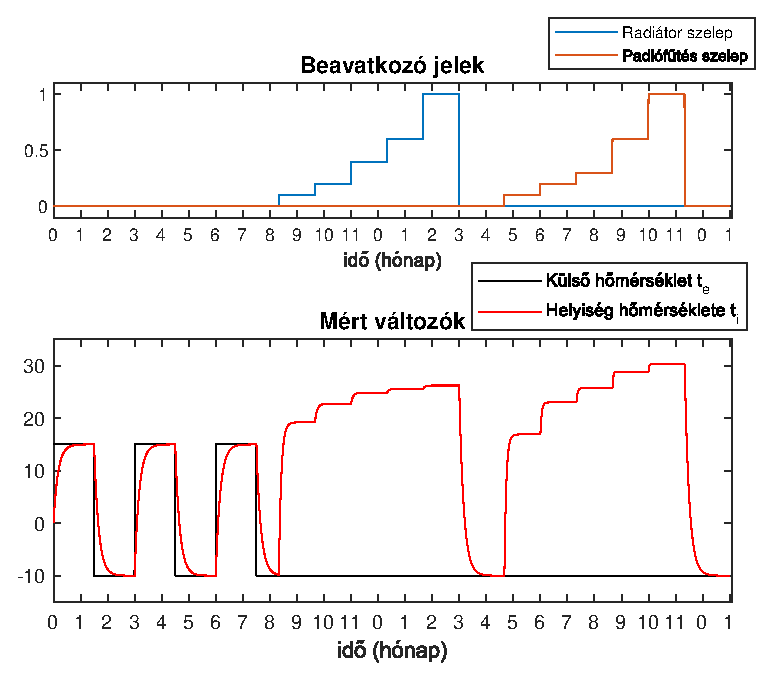
\includegraphics[trim=0 0 0 0, clip,width=0.73\textwidth]{figures/valve-stair}
	\caption{Szimuláció a szelepeket lépcsős függvénnyel gerjesztve}
	\label{fig:valve-stair}
\end{figure}

A fűtőtestekben a víz tömegáramát szelepekkel szabályozzuk. Az \textit{\ref{eq_holeadas4}. egyenlet} adja fűtőtestek által leadott hőmennyiséget, ám ez nem lineáris függvénye a tömegáramnak. A \textit{\ref{fig:valve-stair}. ábrán} látszik, hogy kétszer jobban kinyitott szeleppel $t_i$ belső hőmérséklet végértéke csak kicsivel lesz magasabb. A szelepek tehát nemlineáris bemenetek, a szuperpozíció elve nem működik\footnote{A szakasz másik nemlinearitása a szaturáció: a szelepet csak [0..1] tartományban lehet működtetni -- a szabályzótervezésnél ezt figyelembe fogom venni.}.

A $t_i$ belső hőmérséklet végértéke a tömegáramon kívül a $t_e$ külső hőmérséklettől is függ: ugyanakkora belső hőmérsékletet csak nagyobb tömegárammal, vagy nagyobb $t_w$ előremenő vízhőmérséklettel lehet tartani\footnote{Bár a vízhőmérsékletet nem szabályozom, egyes kazánok rendelkeznek külső hőmérővel, így a vízhőmérsékletet megemelve a hidegben a $t_i$ végértéke "automatikusan" azonos maradhat.}. 

\begin{figure}[H]
	\centering
	% trim={<left> <lower> <right> <upper>}
	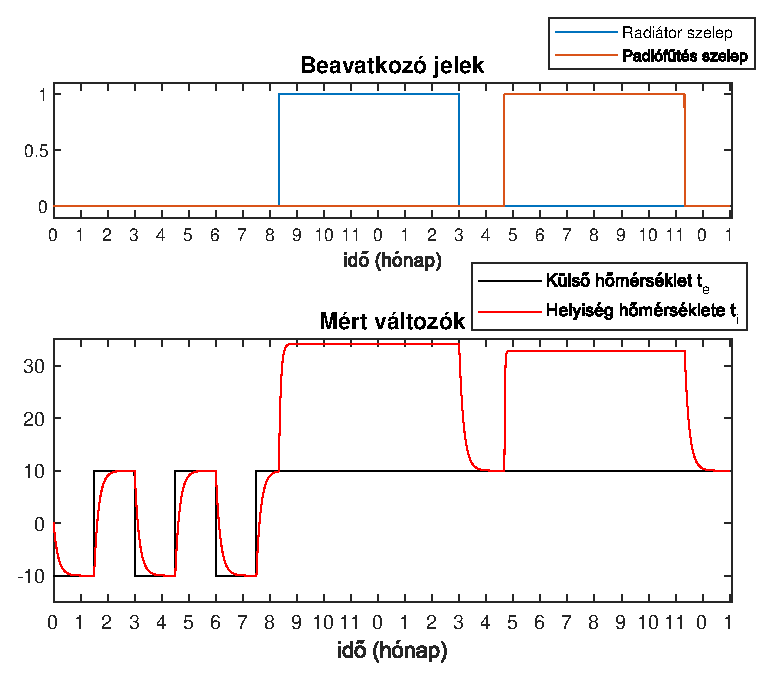
\includegraphics[trim=0 0 0 0, clip,width=0.72\textwidth]{figures/valve-step-hot}
	\caption{Szimulációs eredmények a bemeneteket külön-külön gerjesztve}
	\label{fig:valve-step-hot}
\end{figure}

Látható, hogy a különböző bemenetekre adott gerjesztések hatása a kimeneten sem számítható szuperpozícióval: \SI{20}{\celsius}-kal megemelt $t_e$ külső hőmérséklet esetén a fűtőtestek nem fognak \SI{20}{\celsius}-kal magasabb belső hőmérsékletre fűteni. Ez vonatkozik két szelep együttes kinyitására is: a hőmérséklet nem fog jelentősen megemelkedni.

A fenti hatásokat nemlineáris modellekkel lehetne lekövetni, viszont az ezekkel kapcsolatos (hiányos) ismereteim miatt erre szabályzótervezéssel nem próbálkoztam. Viszont egy nemlineáris modellt tudtam identifikálni a mérési adatokra, ami a fenti problémák egy részét kiküszöbölte.

%A Simulink modellt bemenetein gerjesztem (külső hőmérséklet \SI{40}{\celsius}, majd fűtés \SI{60}{\celsius} előremenő hőmérsékleten valve = 1 állásban.\footnote{A stratégia lehet $t_s$ előremenő hőmérséklet vagy $\xi \cdot \dot m$ tömegáram szabályzása $\alpha$ = [0..1] beavatkozójellel. })

\section{Átviteli függvény illesztése az adatokra}

Az identifikációhoz adatfájlt hozok létre, a Simulinkben IDDATA blokk a be- és kimenetek értékét mintavételi időnként rögzíti és a \textit{Base Workspace}-be (a közös változók közé) menti. Innen a \textit{System Identification} alkalmazásba betölthetőek az adatok. %A mintavételi idő először egy másodperc volt. %A Matlab Workspace-ben megjelenik egy iddata, ezt tudom az ident toolboxba importálni.
Az adatsorra átviteli függvényeket illesztek: a pólusok, zérusok a száma a Simscape modell alapján meghatározható, RC-hálózatok analógiájával. Ekkor például a radiátorok felmelegedési idejét is leköveti a modell. A teljes helyiség időállandójához képest viszont például a radiátor felmelegedése elhanyagolható. Fél órás mintavételi idő esetén a fűtőtestek egytárolós taggal helyettesíthetők. 




Célszerű az identifikációnál minél nagyobb változásokat mérni - így a rendszer teljes dinamikáját, hőtároló képességét mértem. A beállási idők körülbelül 30 naposak voltak és több periódusnyi mérésre volt szükség. 


%Nem tartottam "értelmét" 1\si{\celsius}-os step jelre identifikálni. Így beállítottam nulla kezdeti értéket a ház összes paraméterére. (Falak, fűtési rendszer, stb. Nyilvánvaló, hogy ilyenkor nem a realizmus a cél, hiszen a nagy változásokra jön elő a rendszer dinamikája.) Nulla kezdeti értékből a környezeti hőmérsékletet 0-ról 40\si{\celsius}-ra emeltem, ennek a beállási ideje több nap volt, majd visszaállítva 0\si{\celsius}-ra megvártam a lecsengést, ezután pedig a beavatkozó szelepeket teljesen kinyitottam. 

%Egy ilyen szimuláció a fenti szekvenciával kb. 50 napnyi viselkedést fog át, ez másodperces mintavételi idővel rengeteg adat, amivel meggyűlik az Ident Toolbox baja is.

%5 perces mintavételi időkkel már sokkal gyorsabban lefut a Simulinkben a szimuláció és a toolboxban az identifikáció, lénygében azonos eredményt adva.

%Viszont a mintavételi idők megváltoztatásánál, nem volt egyértelmű, hogyan reagál a Simscape vagy az MPC. A Simscape-nél kiderült, hogy a mintavételi időt manuálisan nem lehet megadni.


\begin{figure}[H]
	\centering
	% trim={<left> <lower> <right> <upper>}
	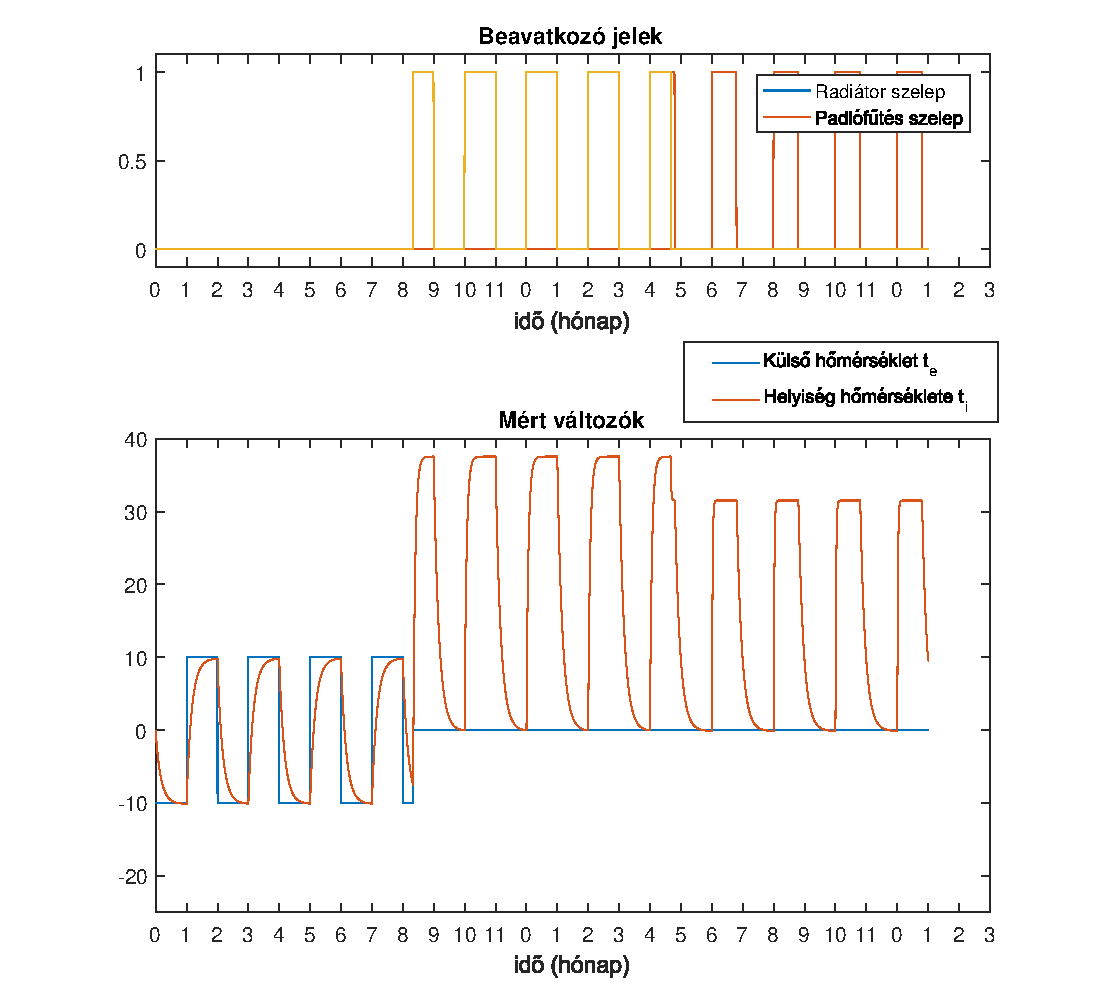
\includegraphics[trim=0 0 0 0, clip,width=\textwidth]{figures/ident-valve3}
	\caption{Identifikáció során }
	\label{fig:ident}
\end{figure}

Az identifikáció pontosságának javításához mindhárom bemeneti változó hatását több periódusra rögzítettem, 750 napnyi szimulációval. Ez fél órás mintavételi idő mellett szimulációban kevesebb, mint 1 perc alatt futott le. Az identifikációhoz a hőmérsékletet kelvinben rögzítem, mivel \si{\celsius} használata esetén az összefüggések nem lineárisak. (A kelvinben mért hőmérsékletet nevezik termodinamikai hőmérsékletnek.) A fenti esetben a beállási idők nagyjából 30 naposak az egész rendszert tekintve, ami 10 nap körüli időállandót jelent. Szakirodalom szerint a falszerkezetek időállandója megközelítőleg 5 nap, a helyiségre így reálisnak tűnik a közelítés.

Átviteli függvény identifikációjához a fenti nemlinearitásokat okozó gerjesztéseket nem vettem figyelembe. Így az átviteli függvény a rendszer jellegét követte, és a \textit{\ref{fig:valve-step-hot}. ábrán} látható külső hőmérsékletre és teljesen kinyitott szelepekre a végértékek pontosan illeszkednek.


\begin{figure}[H]
	\centering
	% trim={<left> <lower> <right> <upper>}
	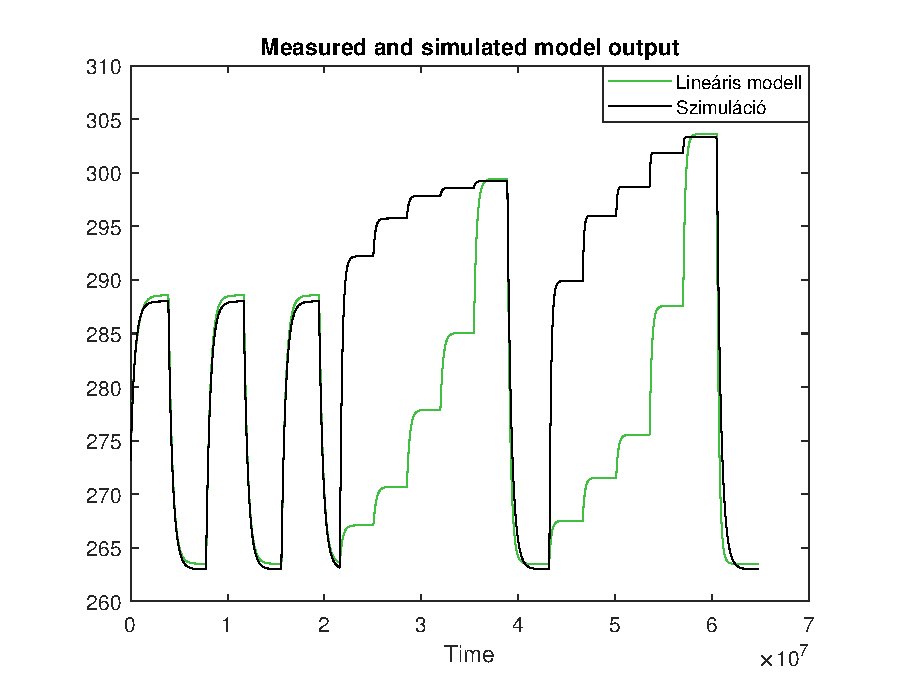
\includegraphics[trim=0 0 0 0, clip,width=0.9\textwidth]{figures/identModelOutputMatch}
	\caption{Identifikált modell pontatlansága}
	\label{fig:ident-model-mismatch}
\end{figure}

%Zérusok hatása röviden. Mit tud. Hánytárolós rendszer. Néhány kép.
%MISO identifikáció. 
%
%
%\section{Hagyományos szabályzás performanciája}
%
%PI, miért nem jó
%Csak SISO-ra működik és itt esetünkben itt több bemenetről van szó mindenképpen. Irodalom: S. Prívara et al. 
%


\pagebreak
\chapter{Szabályzó kiválasztása és analízise}\label{chap:control}

A fejezetben a Simulinkben átviteli függvényre megtervezem a szabályozást. A szabályzó választásakor világossá vált, hogy egy egyszerű PID típusú szabályozás nem képes a rendszert jól kezelni. Igaz, hogy a PID közismert és az iparban egyszerűsége miatt széles körben használt, de épületgépészeti alkalmazásnál egy szabályozás jóságát többféleképp is értelmezhetjük\footnote{Mást tekintünk jó szabályozásnak egy tisztatérben, egy irodában, vagy egy nagyelőadóban, hiszen mások a felmerülő igények, és így a kritériumok is.}. Egyes esetekben hibahatárt megszabva lazíthatunk például a referenciakövetési feltételeken.

Az identifikált modellre többféle szabályzót tervezek, illetve próbálok ki.

A hasonló feladatokra leggyakrabban modell-prediktív (MPC) szabályozást használnak \cite{AFRAM2014343}. Ehhez szükség van a szakasz modelljére, ami alapján a szabályzó szimulálhatja a szakasz kimenetét. Az MPC egy beavatkozójel kiadása előtt több mintavételi perióduson, egy predikciós horizonton keresztül fut le, minden lehetséges  beavatkozójel-sorozatra a kimenetet szimulálva.
%A csúszóablak miatt receding horizon control
Ezen sorozatok közül a legjobbat kiválasztja és egy lépést végrehajt. Ezután a szimuláció újrakezdődik. A végrehajtott, adott horizonton optimális beavatkozójelet egy költségfüggvény minimalizálásával kapja. A költségfüggvényben különböző eltéréseknek vagy abszolútértékeknek különböző súlya lehet.

A szabályozás tehát képes egy horizontig előre tekinteni, és azon belüli optimális beavatkozást végrehajtani. (Az angol nyelvű irodalom erre \textit{receding horizon} névvel hivatkozik.) Az optimalizációt minden mintavételkor végrehajtja, így képes korrigálni, ha a jósolt kimenet és a tényleges kimenet eltérő.

A zárt szabályozási körben a stabilitás viszont nem garantált, erre külön módszerek léteznek (úgynevezett \textit{terminal cost}, azaz végső költség, illetve időben változó súlyozás). Mivel a vizsgált rendszerem nyílt körben is stabil, ezekkel nem kell foglalkoznom.

A stabilitás a beavatkozó jelek és a zavarjel (külső hőmérséklet) korlátosságából fakad. Ezeket is be lehet állítani a szabályzón, így az MPC a szelepekre csak 0 és 1 közötti beavatkozó jelet fog kiadni. A változások hatásait is figyelembe vehetjük, mivel a szelepeket 4-5 perc teljesen kinyitni.

A helyiség hőmérséklet-szabályozásakor a legfontosabb feladat a költségfüggvény súlyainak helyes beállítása\footnote{A súlyozást kiegészíthetik a fizikai korlátok is. Ha a szelepek nyitási- és zárási sebessége korlátos, akkor ezt nem lehet túllépni alacsony súly használatával sem.}. Ezek ugyanis befolyásolják a referenciakövetést - az állandósult állapotbeli hibát és lengést - és a beavatkozójel nagyságát, frekvenciáját is.

Az épületgépészeti rendszereknél a nagyobb frekvenciájú beavatkozójel könnyedén jelenthet alacsonyabb hatásfokot. Viszont ha megengedünk valamennyi ingadozást állandósult állapot körül, a terhelést kiegyenlíthetjük.
Egy irodában, vagy lakásban  például 0.1\si{\celsius}-os vagy 1\si{\celsius}-os pontosságú hőmérséklet-szabályozás közötti különbség komfortban aligha érezhető.
\vspace{6pt}

\begin{figure}[h]
	\centering
	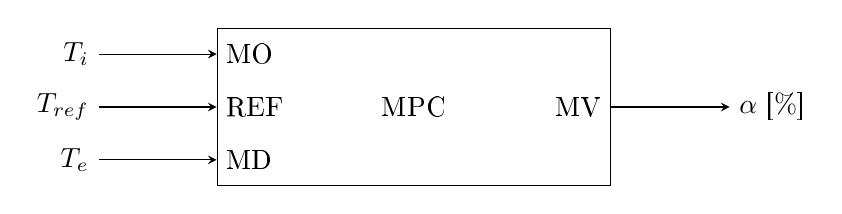
\begin{tikzpicture}[>=stealth]
	% Controller
	% ----------
	\node[draw,rectangle, minimum height=2cm,minimum width=5cm,
		  %label={[xshift=1.0cm, yshift=0.3cm]Label},
		  %label={[xshift=-4.1cm, yshift=-0.7cm]Label},
		  ]
		  (MPC) at (2.3,2.5) {\parbox{2cm}{\centering MPC}};	
	
	% az MPC doboz bemenetei
	\draw [<-] (MPC.165) node[right]{MO} -- +(-15mm,0) node[left]{$T_i$};
	\draw [<-] (MPC.180) node[right]{REF} -- +(-15mm,0) node[left]{$T_{ref}$};
	\draw [->] (MPC.0) node[left]{MV} -- +(15mm,0) node[right]{$\alpha$ [\si{\percent}]};
	\draw [<-] (MPC.195) node[right]{MD} -- +(-15mm,0) node[left]{$T_e$};
	
	\end{tikzpicture}

	\caption{Az MPC be- és kimenetei}
	\label{fig_mpcinout}
\end{figure}

\vspace{6pt}

\begin{table}[H]
	\footnotesize
	\centering
	%\renewcommand{\arraystretch}{2} % to increase cell height
	%\taburulecolor{gray}
	%\begin{tabular}{|p{0.8cm}|p{1cm}|p{1cm}|p{1cm}|p{1cm}|p{1cm}|p{1cm}|p{1cm}|}
	%
	%\begin{tabulary}{\linewidth}{LLc}
	\begin{tabu}{@{}cll@{}}
		\hline
		MPC 	& model predictive control 		& modell-prediktív szabályozás
		\\
		MO / OV	& measured output, output variable 	& mért kimenet (szabályzott jellemző)
		\\
		MD		& measured disturbance			& mért zavarás 
		\\
		MV		& manipulated variable			& beavatkozó jel
		\\
		REF 	& reference signal 				& referenciajel
		\\
		$T_s$ 	& sampling time					& mintavételi idő
		\\ 
		p 		& prediction horizon 			& predikciós horizont 
		\\ 
		c 		& control horizon				& szabályozási horizont
		\\
		J 		& cost function 				& költségfüggvény
		\\
		$w_u$ 	& weight (control signal) 		& beavatkozó jelet büntető együttható
		\\ 
		$w_{\Delta u}$ 	& weight (rate of control signal) 		& beavatkozó jel változását bünteti
		\\ 
		$w_y$ 	& weight (measured output) 		& hibajelet büntető együttható
		\\
		SF 		& scale factor 			& skálázási tényező
		\\    \hline
	\end{tabu}
	\label{tab:MPCvariables}
	\caption{A fejezetben ismertetett rövidítések és angol szakkifejezések}
	%
	%\label{tab:TabularExample}
	%\tabref{TabularExample}~táblázat
\end{table}
\vspace{10pt}



\section{Elvárások a szabályozás teljesítményével szemben}

Az MPC hangolása során % működését, tulajdonságait meg tudjam figyelni,
lépésről lépésre fogom módosítani az alapértelmezett paramétereket, azok hatását megfigyelem.
Az MPC szintézis folyamata a következő:% be kellene tabolni


\begin{enumerate}[noitemsep,topsep=0pt,parsep=2pt,partopsep=4pt,leftmargin=30pt]
	\item a szakaszt identifikálni kell, az átviteli függvény be- és kimeneteinek típusát be kell állítani,
	\item létre kell hozni az MPC-t a megfelelő mintavételi frekvenciával,
	\item be kell állítani a jelek fizikai korlátait és súlyukat a szabályozás költségfüggvényében,
	%\item Be kell állítani a jelek fizikai korlátait
	\item hozzá kell adni a Simulink modell saját változói közé (Model workspace) a szabályozót és megadni a nevét az Explicit MPC blokkjában (az itt található Review funciót is érdemes használni),
	\item be kell kötni a jeleket és le kell futtatni a szimulációt.
	
\end{enumerate}

%Identifikálni kell a szakaszt.

A \verb|"setmpcsignals()"| függvény használatával egy új átviteli függvényt hozunk létre, amit az MPC függvénynek odaadhatunk. Ez annyival több az identifikált átviteli függvénynél, hogy benne vannak a be- és kimenetek típusai is, aszerint, hogy az említett jelek milyen típusúak. A szakasz átviteli függvényének be-~és kimeneteit meg kell nevezni (\verb|MO, MD, MV|) Ezután az \verb|"mpc(tf, Ts)"| függvénnyel létrehozhatjuk az MPC szabályozót a megadott szakaszmodellre.



%Alapértelmezés szerint a költségfüggvény súlyai az alábbiak. A zárt szabályzási körben ezek a súlyok a hibajelet büntették a legjobban, ezért nagyon jó referenciakövetést sikerült elérni.
%
%
%Követelmények a referenciajelekre:
%
%Thermal comfort - Olesen, ISO EN 7730
%
%Floor temperature - herz-ől is
%


%Az MPC szabályzót létrehoztam a toolbox-szal, az identfikált szakaszból. Beállítottam a be-és kimenetek jellegét, korlátait. A ki-és bemeneteket helyesen bekötve már működött is a szabályzás.
%Fontos, hogy helyesen válasszuk meg a mintavételi időt, illetve a súlyokat

%A kezdeti cél egy "sima" szabályzás. Kérdés, hogy egyáltalán tud-e ilyet az MPC. Gyanítom, hogy a hibaminimalizáló függvény megfelelő megadásával tud: ha egy négyzetes hibaminimalizáló van rajta, \textit{biztosan "jó"} lesz.\footnote{Bármit is jelentsen a \textit{jó} szabályzás.}


%A fenti a klasszikus MPC, tov. info. Baochang DING, Modern MPC című könyvében olvasható.

\section{A létrehozott MPC tulajdonságai}

Az \verb|"mpc()"| függvény még nem ad azonnal használható szabályzót. Az alapértelmezett súlyok és a normalizálatlan bemenetek miatt a legkisebb költségű beavatkozás akár az is lehet, hogy a szabályzó nagy követési hiba ellenére nulla beavatkozó jelet ad ki.

A költségfüggvény akkor működik jól, ha a modellbemeneteket normáljuk. Be kell állítani az MPC mért változóinak tulajdonságánál a modell kimenetének  skálázását, amit az állandósult állapotbeli értékek, illetve a jellemző változásoknak megfelelően kell beállítani.

A helyiség modelljénél nagy eltérések vannak, hiszen a szelepek normálva vannak, a hőmérséklet értékeket viszont kelvinben értelmezem. Így a skálafaktort a 30..300 közötti nagyságrendben célszerű választani, mivel a hőmérsékletértékek nagyságrendileg \SI{30}{\degreeCelsius}-nyi tartományban változnak.

A Simulinkben identifikált modell egy munkapont körül (adott környezeti hőmérséklet mellett) volt csak pontos, ám ez a referenciakövetést nem rontotta el. A szabályozás megváltozott paraméterekkel is működött a Simscape hálózatra, a referenciakövetés minősége megmaradt.


%\begin{itemize}[noitemsep,topsep=-8pt,parsep=0pt,partopsep=0pt]
%	\item A mintavételi idő növelése az MPC-ben magával vonja, hogy az a Simulink blokkban is módosul. 
%	\item A Simulinkben az időt a jobb alsó sarokban mindig mp-ben írja ki. Ámde ha a steppingnél 1000 step-et állítok be, az a jobb alsó sarokban $T_s$-sel felskálázva fogja a mp-t mutatni. Azaz 5 perces sampling time esetén 1 step a jobb alsó sarokban T=300 mp-nek felel meg.
%	\item A mintavételi idő megválasztása nagyban meghatározza a költségfüggvény értékét.
%\end{itemize}



\subsection{Módosítások az MPC-ben}

A súlyozást módosítva adhatunk költséget a beavatkozásnak, csökkentve így például annak a frekvenciáját. Ez a referenciakövetést rontja, de esetünkben nem cél a tized \si{\celsius}-os pontosság, hanem az energiamegtakarítás.
Pontosan fel kellene ezért írni a forintosított költségét a beavatkozásnak, és ezt minimalizálni. Ez viszont egy összetett kapcsolat és jelentősen függ az épületgépészettől. Így általánosan fogom a paraméterváltozások hatásait vizsgálni.

\subsection{Az MPC költségfüggvénye}


A szabályzó a predikciós horizonton belül minden lehetséges beavatkozójel-sorozatra kiszámolja annak (várható, modell szerinti) költségét. Azt a beavatkozójel-sorozatot választja, ami a legkisebb költséggel jár. Ez után a szabályozási horizontnak megfelelő számú beavatkozást végez, nem adja ki a teljes sorozatot. 

%A legbutább szabályzó szabályzási és predikciós horizontja is 1. Azaz egy lépéssel lát előre és a legkedvezőbb esethez (J költség minimális) tartozó beavatkozó jelet végrehajtja\footnote{Ezt formalizálni kellene egyenletben is.}. $J=w_u u + w_e e$, ahol a hibát a szabályzóban lévő szakaszmodell alapján számítjuk.
\textit{Agachi \cite{romanMPC_Agachi}} szerint:

\begin{equation} \label{eq_mpc_cost}
J = \sum_{i}^{p} \left(w_u \Delta u^2 + w_e (r_i-y_i)^2  \right)
\end{equation}

%(itt még csak $r_i=r$ állandó referenciajellel tudtam csinálni. )
ahol N a predikciós horizont, $w_u$ a beavatkozó jel változásának súlya, $w_e$ a hibajel súlya. A referenciajel jövőbeli változásait figyelembe lehet venni a predikciós horizonton belül\footnote{A jövőbeli változásokat ismerhetjük, ha van egy referenciajelünk, vagy lehet becslés rá egy időjárás-előrejelzés.\\Bővebben az elméletről: https://www.mathworks.com/help/mpc/ug/signal-previewing.html,\\illetve a felhasznált Simulink blokkok: https://www.mathworks.com/help/mpc/examples/improving-control-performance-with-look-ahead-previewing.html}.

A költségfüggvényben a hibajelhez és beavatkozó jelekhez, illetve azok változásaihoz különböző súlyok tartozhatnak.
Nagyobb súlyok nagyobb költséget eredményeznek, így a szabályozó a nagyobb költségű beavatkozójel-sorozatot kisebb valószínűséggel választja.

\begin{figure}[H]
		\centering
		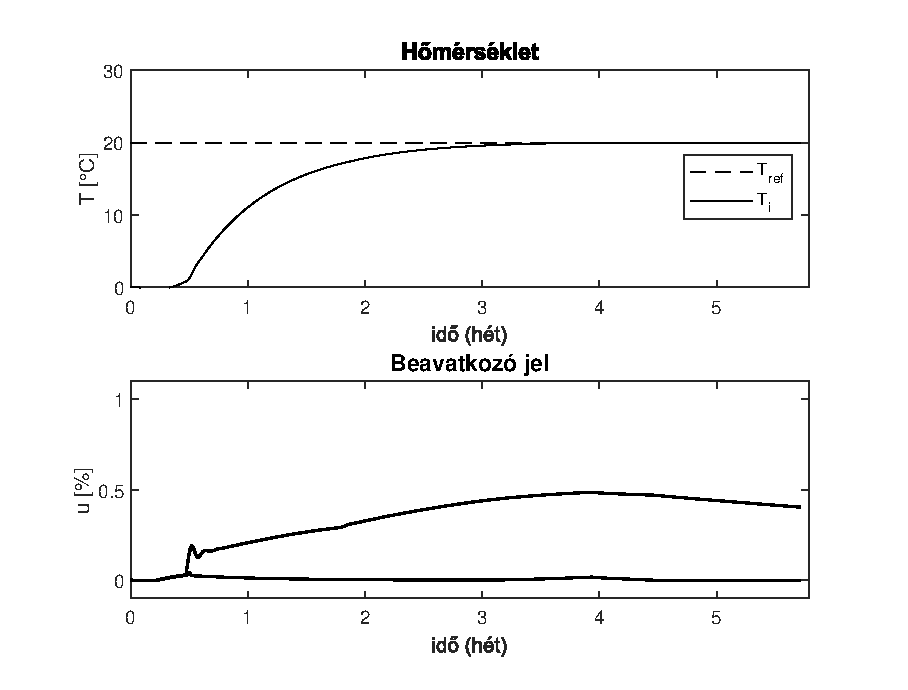
\includegraphics[width=0.8\textwidth]{figures/simscape/mpc}
		\caption{A zárt szabályozási kör ugrásválasza}
		\label{fig:mpc-simulated}
\end{figure}

A fenti ábrán látható a helyesen súlyozott MPC-vel a zárt szabályozási kör viselkedése. Ebben vannak tökéletlenségek, ezekre a fizikai modellnél térek majd rá. A szabályozó paraméterei az alábbi táblázatban láthatók.
\begin{table}[H]
	\footnotesize
	\centering
	%\renewcommand{\arraystretch}{2} % to increase cell height
	%\taburulecolor{gray}
	%\begin{tabular}{|p{0.8cm}|p{1cm}|p{1cm}|p{1cm}|p{1cm}|p{1cm}|p{1cm}|p{1cm}|}
	%
	%\begin{tabulary}{\linewidth}{LLc}
	\begin{tabu}{@{}cl@{}}
		\hline
		$T_s$ 	& 1800 s
		\\ 
		p 		& 50 minta (25 óra)
		\\ 
		c 		& 1
		\\
		$w_u$ 	& 0.005 
		\\ 
		$w_{\Delta u}$ 	& 50
		\\ 
		$w_y$ 	& 20
		\\
		SF 		& 30 
		\\   \hline
	\end{tabu}
	\label{tab:MPCfactors}
	\caption{MPC szabályozó paraméterei}
	%
	%\label{tab:TabularExample}
	%\tabref{TabularExample}~táblázat
\end{table}

\subsection{Fejlesztési lehetőségek a szabályozással kapcsolatban}
	
Épületautomatikai rendszerek használatával, például az iContrALL intelligens otthon rendszerével a fellépő zavarásokat (emberek jelenléte, napsütés, szél) mérhetjük. A szabályozás a zavarások hatásmechanizmusának ismeretében jobb zavarelnyomást tud elérni, sőt az integrációval további beavatkozók is használhatók (például árnyékolástechnikai eszközök).


\chapter{Tesztek laborkörülmények között}

\section{A kísérleti rendszer}
Az elméleti eredmények validálásához elkészítettem egy szoba kicsinyített modelljét. Ez egy kartondobozban kapott helyet. A doboz hőtároló képessége elég csekély, ezért extra hőtároló tömegeket helyeztem bele, OSB falapot és egy elektromos kályhából vett samott téglát.
A fűtési teljesítményt halogén izzókkal juttattuk a rendszerbe. Ezek teljesítménye szabályozható, így ez a bemenet lineáris a szelepekkel ellentétben, azaz kétszer nagyobb beavatkozójelre kétszer nagyobb teljesítmény kerül a rendszerbe.
A hőmérsékletet mérjük a dobozban és azon kívül is. Zavarásként a mérőszoba ablakát kinyitjuk, így a doboz környezeti hőmérséklete lecsökken.

\begin{figure}[H]
	\centering
	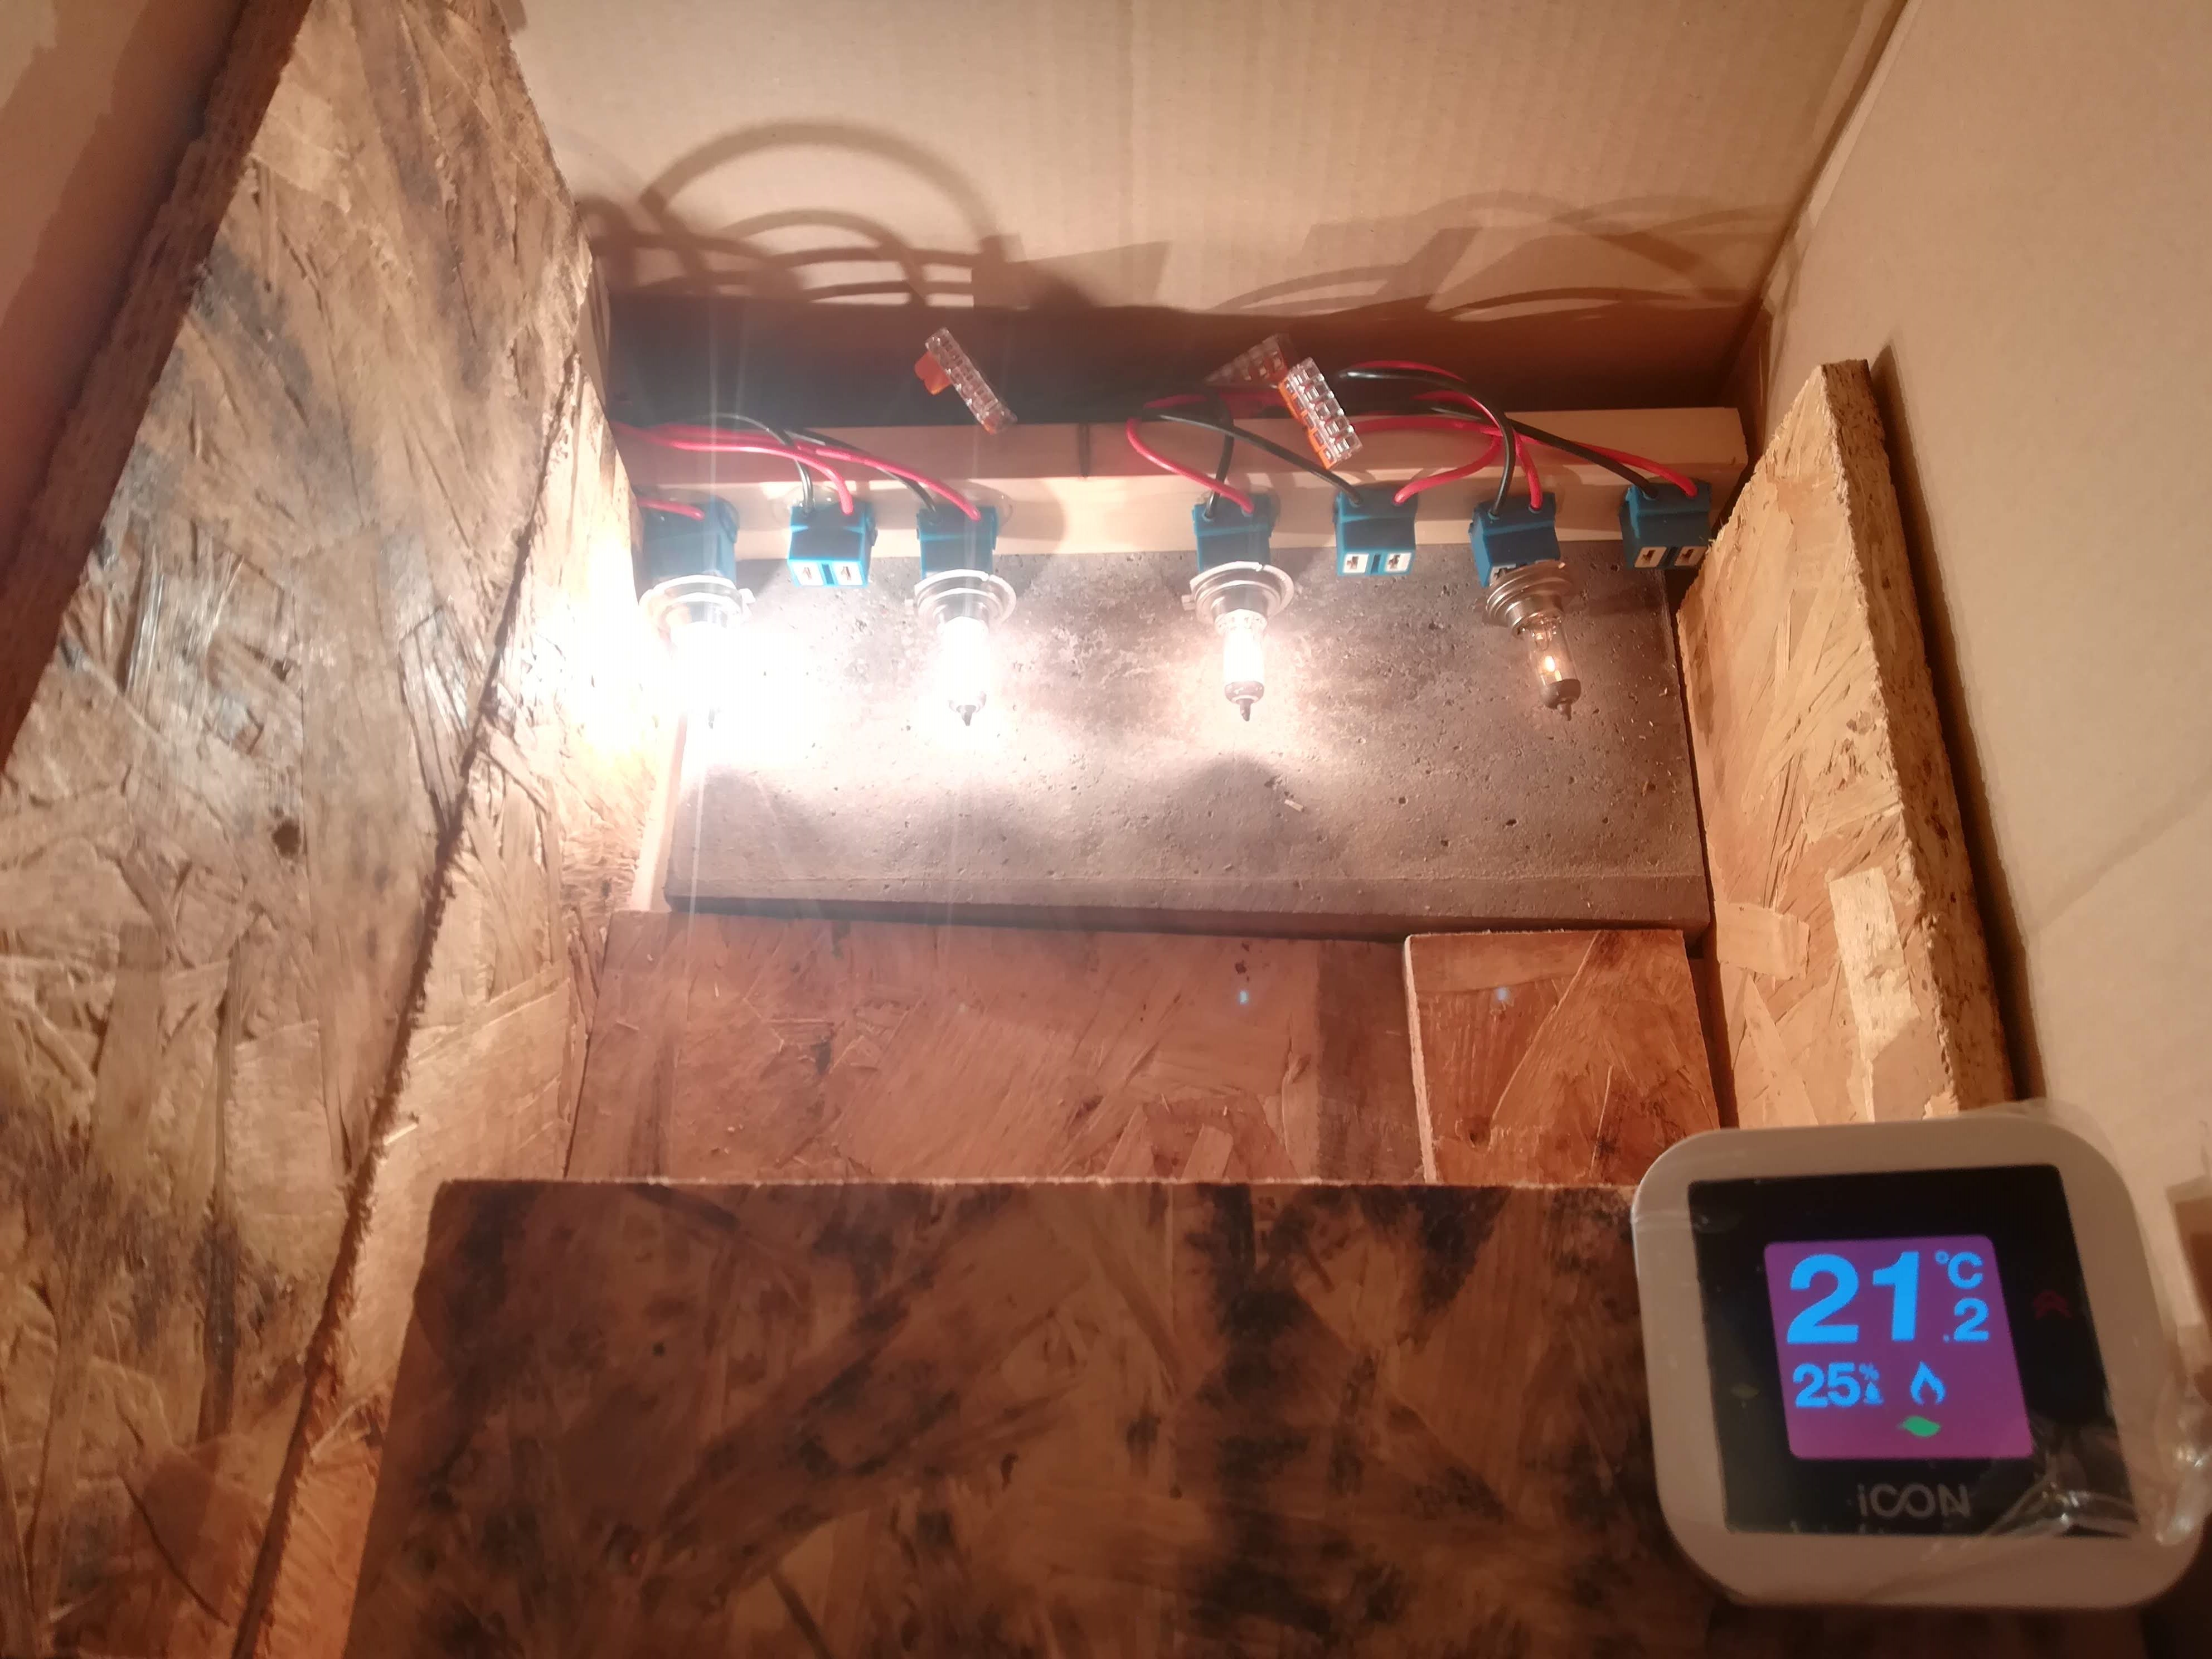
\includegraphics[width=0.8\textwidth]{figures/realsys/interior2}
	\caption{A doboz belseje hőmérővel és szabályozható izzókkal}
	\label{fig:realsys-interior}
\end{figure}

\section{A Simulink konfigurálása}
A valós idejű futáshoz Simulink  Real-time szükséges. A real-time működés itt azt jelenti, hogy a szabályozót a Simulink mintavételi időnként futtatja le. Azaz ha a kísérleti rendszerre \SI{30}{\second}-es mintavételi idejű szabályzót tervezek, akkor az MPC félpercenként mintát fog venni a hőmérsékletekből és ki fog adni egy beavatkozójelet. Így a real-time ez esetben nem jelent például szigorú korlátokat a futásidőre.


%A Real-time UDP-t használom. %https://uk.mathworks.com/help/xpc/io_ref/udp-transport-protocol.html
%https://uk.mathworks.com/products/simulink-desktop-real-time.html

A szabályzó a számítógépen fut, és mintavételi időnként a jelenlegi hőmérsékletet beolvassa, az MPC-t lefuttatja, a beavatkozó jeleket pedig elküldi a beágyazott számítógépnek.

\begin{figure}
	\centering
	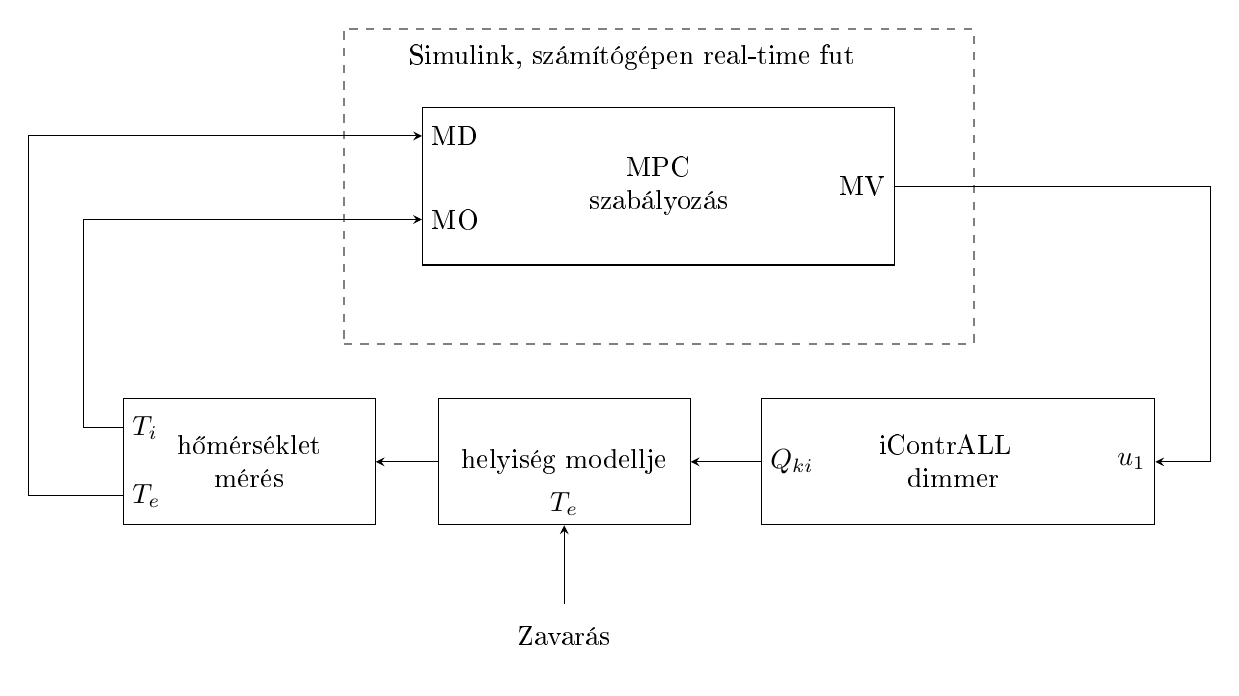
\begin{tikzpicture}[>=stealth,
  		%inner/.style={draw,fill=blue!5,thick,inner sep=3pt,minimum width=8em},
		%outer/.style={draw=gray,dashed,fill=green!1,thick,inner sep=5pt}
		outer/.style={draw=gray,dashed,thick,inner sep=5pt}
		]
	
	% Szabályzási kör elemei
	% ----------------------
	
		% Szabályzó
		\node[draw,rectangle, minimum height=2cm,minimum width=6cm] (MPC) at (3.2,3.5) {\parbox{2cm}{\centering MPC szabályozás}};		

		% Fűtési rendszer
		\node[draw,rectangle, minimum height=1.6cm,minimum width=5cm] (Heat) at (7,0) {\parbox{2cm}{\centering iContrALL~~~~ \\ dimmer~~}};
	
		% Ház
		\node[draw,rectangle, minimum height=1.6cm,minimum width=3.2cm] (House) at (2,0) {helyiség modellje};
		
		% Hőmérő
		\node[draw,rectangle, minimum height=1.6cm,minimum width=3.2cm] (Measure) at (-2,0) {\parbox{2cm}{\centering hőmérséklet\\mérés}};
		
		%Zavarás
		\node[rectangle, minimum height=0.8cm,minimum width=2cm,below=of House, node distance=1cm] (ghostDist)  {Zavarás};

		
	
	% Kiegészítő cuccok
	% ----------------------
	
	% Keret - Matlab
	\node[draw,outer,rectangle, minimum height=4cm,minimum width=8cm,
	label={[label distance=-0.1cm, anchor=north]100:Simulink, számítógépen real-time fut}] (keret) at (3.2,3.5) {};
	
	% Zavarás a modellbemenetre
	\draw[->] (ghostDist.90) --  (House.270) node[above]{$T_e$};
	
	%\draw[->] (ctr.191) node[right]{${u_{2}}$} -| ++(-1.7,1.3)|-  (Numeric.172) node[right]{$\alpha_{floor}$};  %node[above left]{$\alpha_{radiator}$}; 
	
	% mért változók
	\draw[->] (House.180) -- (Measure.0);
	\draw[->] (Measure.195) node[right]{$T_e$} -| ++(-1.2,0)  |-  (MPC.168) node[right]{MD} ;
	\draw[->] (Measure.165) node[right]{${T_{i}}$}-| ++(-0.5,0.8)  |-  (MPC.188) node[right]{MO} ;

	
	%\draw[->] (d.0) node[left]{heat [W]} ->  ++(3,0) ->  (house.180);
	% Beavatkozó jel
	\draw [->] (MPC.0) node[left]{MV} -| ++(4,-2.5)  |- (Heat.0) node[left]{${u_1}$}; %++(1.5cm,0) -- (2cm,0pt) -- (2.5cm,10pt);
	
	\draw[->] (Heat.180)  node[right]{$Q_{ki}$} -- (House.0) ;
	%\draw[->] (d.20) -| ++(1,-1) |- (y.350);
	
	%\path 
	%(d.150)	 edge[<->] 	node[anchor=north,above]{valvePercent}	(y.270);
	
	% Lehetséges label beállítások:
		%label={[blue,yshift=0.3cm]above:Z}]
	
%	\node[draw,outer,rectangle, minimum height=5.5cm,minimum width=13cm,
%	label={[label distance=-0.1cm, anchor=north]270:3 bemenetű, 1 kimenetű szakaszmodell}] (keret) at (0,15) {};
%	
%	
	\end{tikzpicture}

	\caption{A valós idejű mérések szereplői}
	\label{fig:realtimesimulink}
\end{figure}

%\begin{tikzpicture}[>=stealth,remember picture]
%\node[draw,rectangle,inner sep=0.5cm] (y) at (0,0) {$A$};
%\node[draw] (d) at (0,2) {%
%%	\begin{tikzpicture}[remember picture]
%%	\matrix [matrix of math nodes] (mat)
%%	{
%%		B & \phantom{C}   \\
%%		\phantom{B} & C \\
%%	};
%%	\end{tikzpicture}
%%};
%%\draw[->,shorten >= 6pt] (y.west) -| ++(-1,1) |- (mat-1-1);
%%\draw[->,shorten >= 6pt] (y.west) -| ++(-0.8,1) |- (mat-2-1);
%%\draw[->] ($(mat-2-2)+(14pt,0)$) -| ++(0.8,-1) |- (y.east);
%%\draw[->] ($(mat-1-2)+(14pt,0)$) -| ++(1,-1) |- (y.east);
%\end{tikzpicture}




% 3600001117-es ID-jű, Raspberry Pi, IP címe fixen 192.168.0.108, 54321-es port.

%A PI SPI-n küld a rádióadónak.
%Rádiókommunikáció egyirányú.

\section{Szabályozótervezés az identifikált modellre}
Mivel a kísérleti rendszeremnek nincsen energetikai tanúsítványa, identifikáltam az ugrásválaszával (\ref{fig:realsys-ident}. ábra).

\begin{figure}
	\centering
	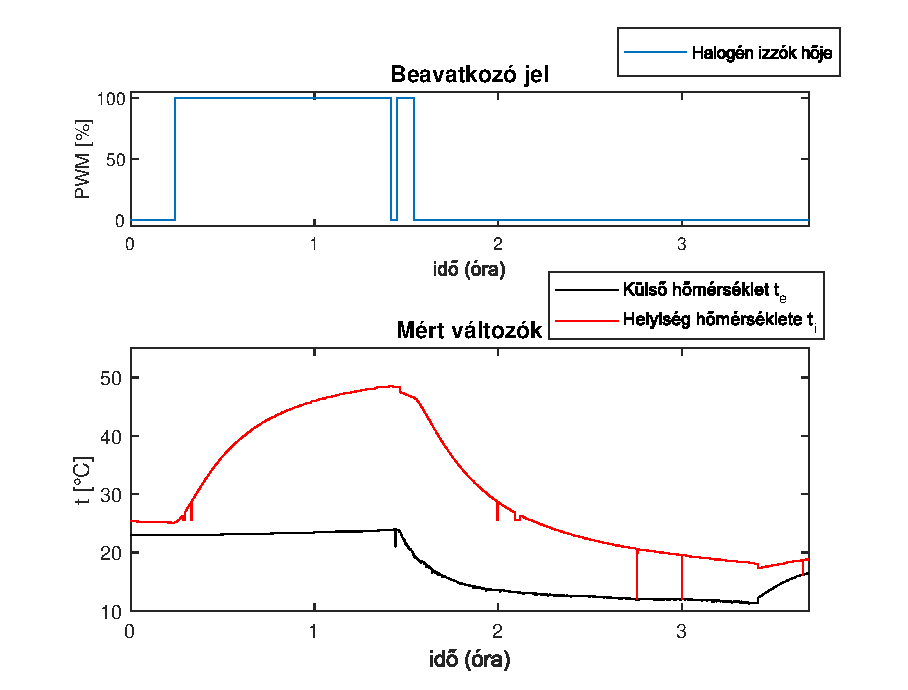
\includegraphics[width=0.65\textwidth]{figures/realsys/ident}
	\caption{Identfikációhoz használt mérési adatsor}
	\label{fig:realsys-ident}
\end{figure}

A valós idejű méréshez használni kívánt szabályozót érdemes először szimulációban megvizsgálni. Ekkor adott a szabályzott szakasz identifikált lineáris modellje, az MPC-t pedig létrehoztam  a modellhez az előző fejezet szerint. Az ott felmerülő nehézségeket, problémákat a fizikai rendszeren szerzett tapasztalatok miatt sikerült megoldani. A Simulinkben a tervezés a \textit{\ref{fig:mpc-sim}. ábra} szerinti elrendezésben történt, használva az MPC szabályozás közbeni (online) hangolásának lehetőségét.



\subsection{Mintavételi idő és predikciós horizont}

Az MPC paraméterezésére \textit{Agachi \cite{romanMPC_Agachi}} könyvében találhatók ajánlások. A predikciós horizontot eszerint úgy kell megválasztani, hogy az a szakasz releváns dinamikáját lefedje. Mivel a felfutási ideje a kísérleti rendszernek körülbelül 1 óra, ezért ezt ekkorára választottam. A predikciós horizont ajánlott nagysága 10-20 mintavétel a számítási igény csökkentése miatt (így $T_s =$ \SI{300}{\second} adódna),  viszont a mérés során gyakrabban szerettem volna látni a változásokat, a mintavételi időt 30 másodpercnek vettem.

\begin{figure}[h]
	\centering
	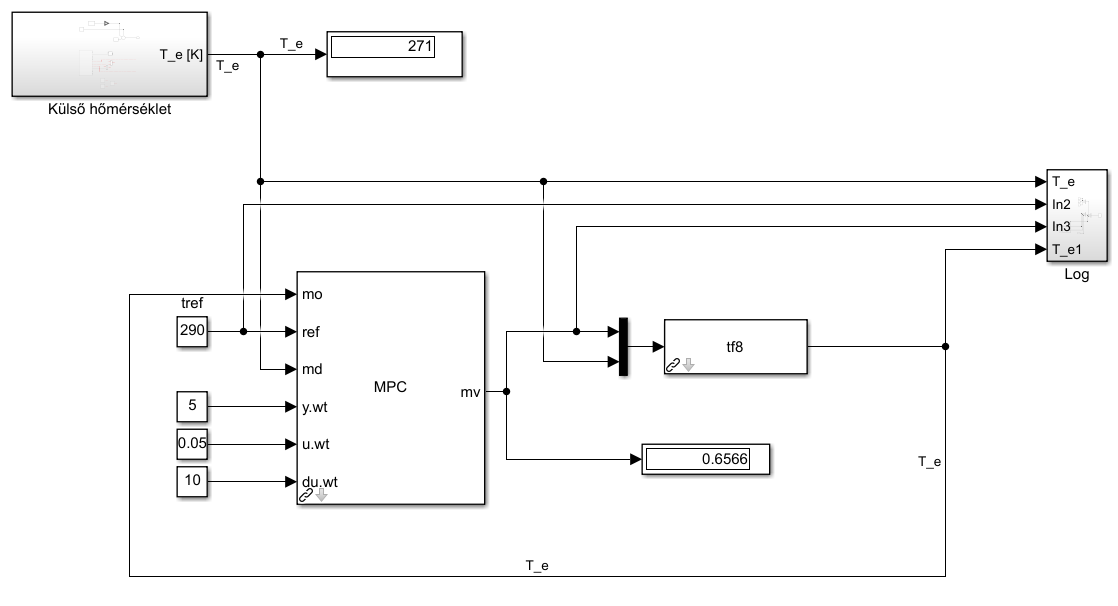
\includegraphics[width=\textwidth]{figures/simscape/simModel}
	\caption{Lineáris modellre MPC szimulációja}
	\label{fig:mpc-sim}
\end{figure}

A fentiek mellett viszont a szabályozó nem adott ki beavatkozójelet egészen egy predikciós horizontnyi ideig, azaz majdnem 1 órán keresztül\footnote{Ha 300 másodperces mintavételi időt használtam és 10 mintányi predikciós horizontot, ugyanez volt a helyzet. Ez idő alatt az MPC valószínűleg az állapotbecslőjét inicializálja.}. Az MPC képes a költségfüggvényben figyelembe venni a predikciós horizonton belül a referenciajel jövőbeli változásait (ez a \textit{Signal Previewing}), ezt kipróbáltam annak érdekében, hogy ezt a \say{holtidőt} csökkentsem, ám ellentétes hatást értem el.

A Simulink blokk viszont támogatja az MPC-nek kezdeti érték megadását. A kezdeti érték nélküli MPC-t szimulációban (azaz nem valós időben) futtattam, majd leolvastam annak belső állapotát. Az \verb|mpcstate| függvénnyel létre kellett hoznom egy objektumot, ami a Simulinkben a szabályzót inicializálja. Ehhez szükség volt a szabályzó állapotteres szakaszmodelljének\footnote{Amikor az MPC-t létrehozzuk, a szakaszmodellt a Matlab állapotteressé alakítja.} becsült állapotára, a zavarjel becsült értékére, a zaj becsült értékére (ez esetben üres vektor), a legutóbbi beavatkozójelre és egy kovarianciamátrixra (ezt nullmátrixnak vettem).

Azzal, hogy a fenti objektumban a legutóbbi beavatkozójelet maximálisnak vettem, valós idejű futás esetén, a fizikai rendszer ugrásválaszánál nem kellett kivárnom egy órát, azaz a predikciós horizontnyi időt, hanem a szabályzó rögtön maximális beavatkozójelet adott ki.

\subsection{A szabályozó költségfüggvénye}

A költségfüggvény súlyait iteratívan választottam ki. A paraméterek akár a szabályozó futása közben is módosíthatók, hatásuk azonnal látható. Először a referenciakövetést leginkább befolyásoló $w_y$ paramétert állítottam be.
 
\begin{figure}[H]
	\centering
	% trim={<left> <lower> <right> <upper>}
	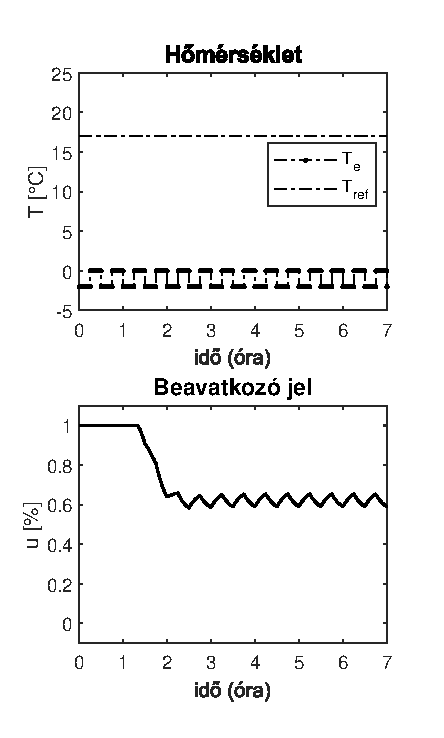
\includegraphics[width=0.4\textwidth, trim=0 168 0 0, clip,]{figures/realsys/disturbpar}
	\caption{Referenciajel és zavarás a szimuláció során}
	\label{fig:mpc-dist}
\end{figure}

\begin{figure}[H]
	\begin{subfigure}[t]{0.32\textwidth}
		\centering
		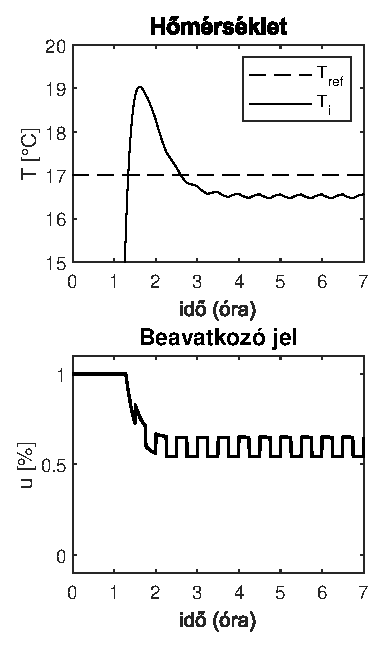
\includegraphics[width=\textwidth]{figures/realsys/mpc-wy-1}
		\caption{$w_y=1$}
		\label{fig:mpc-wy-1}
	\end{subfigure}
	~
	\begin{subfigure}[t]{0.32\textwidth}
		\centering
		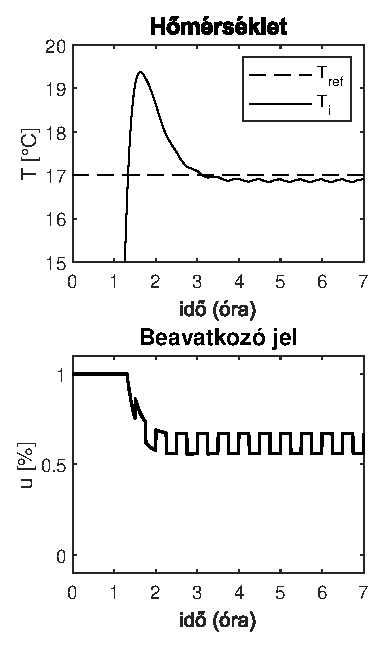
\includegraphics[width=\textwidth]{figures/realsys/mpc-wy-2}
		\caption{$w_y=2$}
		\label{fig:mpc-wy-2}
	\end{subfigure}
	~
	\begin{subfigure}[t]{0.32\textwidth}
		\centering
		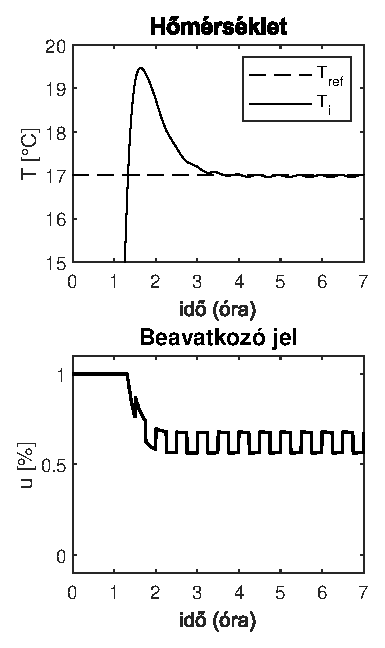
\includegraphics[width=\textwidth]{figures/realsys/mpc-wy-5}
		\caption{$w_y=5$}
		\label{fig:mpc-wy-5}
	\end{subfigure}
	\caption{MPC viselkedése különböző $w_y$ értékekre}
	\label{fig:mpc-wy}
\end{figure}

A \ref{fig:mpc-wy-5}.~ábrán látható esetben volt a legjobb a referenciakövetés, így ezt a paramétert rögzítettem. Következőnek a $w_u$ paraméter értékét választottam meg. Ez a beavatkozójel nagyságát bünteti.

\begin{figure}[H]
\begin{subfigure}[t]{0.32\textwidth}
	\centering
	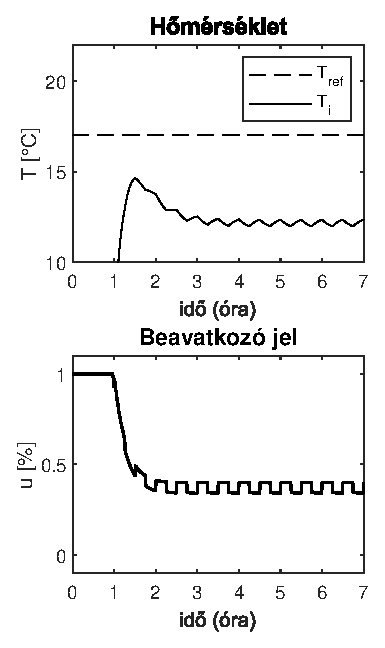
\includegraphics[width=\textwidth]{figures/realsys/mpc-wu-20}
	\caption{$w_u=20$}
	\label{fig:mpc-wu-20}
\end{subfigure}
~
\begin{subfigure}[t]{0.32\textwidth}
	\centering
	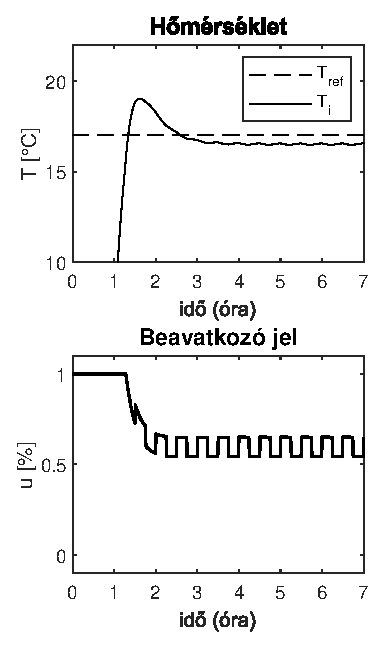
\includegraphics[width=\textwidth]{figures/realsys/mpc-wu-05}
	\caption{$w_u=5$}
	\label{fig:mpc-wu-05}
\end{subfigure}
~
\begin{subfigure}[t]{0.32\textwidth}
	\centering
	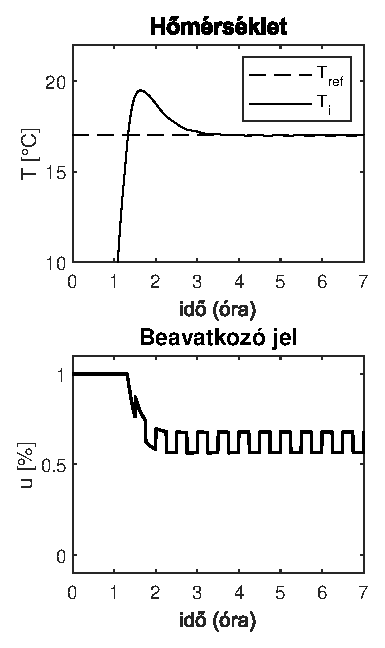
\includegraphics[width=\textwidth]{figures/realsys/mpc-wu-005}
	\caption{$w_u=0.05$}
	\label{fig:mpc-wu-005}
\end{subfigure}
\caption{MPC viselkedése különböző $w_u$ értékekre, $w_y=5$ mellett}
\label{fig:mpc-wu}
\end{figure}
 A \ref{fig:mpc-wu}.~ábrán látható, hogy nagy súly a költségfüggvényben lecsökkent beavatkozójelet, és így nagy követési hibát okoz. A két felsorolt paraméter valójában egymás ellenében hatnak\footnote{Bővebben a paraméterekről: https://uk.mathworks.com/help/mpc/ug/tuning-weights.html}.

A beavatkozást kevésbé büntettem, így a referenciakövetés megmaradt, viszont a túllövés lecsökkent. Most már két fix paraméter mellett választottam súlyt a beavatkozójel változási sebességéhez.

\begin{figure}[H]
\begin{subfigure}[t]{0.32\textwidth}
	\centering
	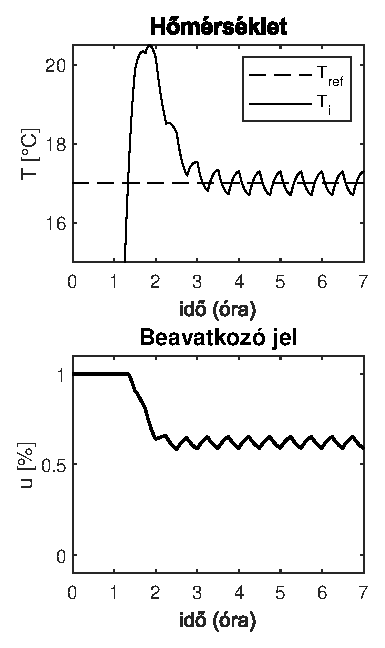
\includegraphics[width=\textwidth]{figures/realsys/mpc-wdu-100}
	\caption{$w_{\Delta u}=100$}
	\label{fig:mpc-wdu-100}
\end{subfigure}
~
\begin{subfigure}[t]{0.32\textwidth}
	\centering
	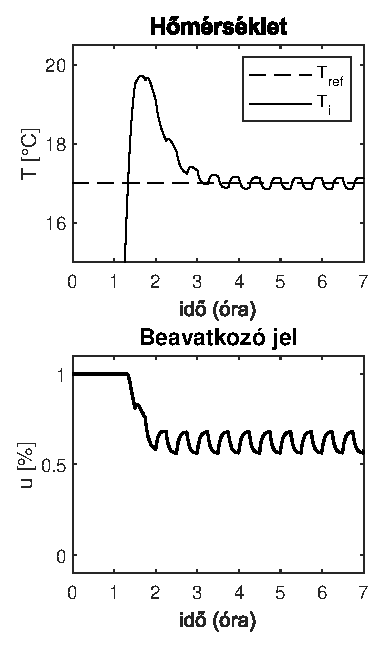
\includegraphics[width=\textwidth]{figures/realsys/mpc-wdu-50}
	\caption{$w_{\Delta u}=50$}
	\label{fig:mpc-wdu-50}
\end{subfigure}
~
\begin{subfigure}[t]{0.32\textwidth}
	\centering
	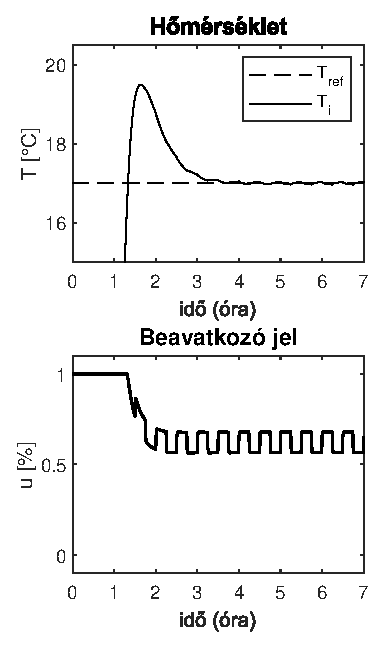
\includegraphics[width=\textwidth]{figures/realsys/mpc-wdu-10}
	\caption{$w_{\Delta u}=10$}
	\label{fig:mpc-wdu-10}
\end{subfigure}
\caption{MPC viselkedése  $w_{\Delta u}$ értékekre, $w_y=5$, $w_u=0.05$ mellett}
\label{fig:mpc-wdu}
\end{figure}

\begin{figure}[H]
	\centering
	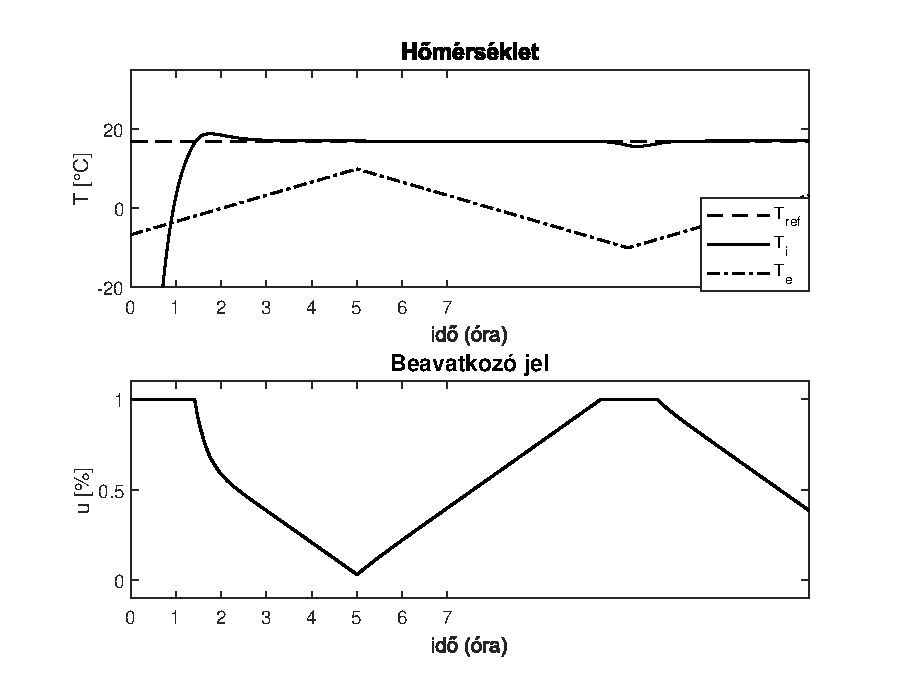
\includegraphics[width=0.7\textwidth]{figures/simscape/distrej}
	\caption{A zárt szabályozási kör ugrásválasza}
	\label{fig:mpc-distrej}
\end{figure}

A \ref{fig:mpc-wdu}. ábrán jól megfigyelhető, hogy nagy súly esetén a beavatkozójel frekvenciája lecsökken\footnote{A beavatkozás alapfrekvenciáját a \textit{\ref{fig:mpc-dist}. ábra} szerinti zavarjel adja, viszont a felfutás sebessége a $w_{\Delta u}$ paramétertől függ.}. Ez az épületgépészeti rendszerekben alacsonyabb energiafelhasználással járhat. Ám a három esetben különböző mértékű lengés tapasztalható állandósult állapotban: ezek közül az igényeknek, illetve a specifikációnak megfelelőt kell kiválasztani. A zavarelnyomást megvizsgáltam nagyobb tartományban változó külső hőmérséklettel is, ez látható a \textit{\ref{fig:mpc-distrej}. ábrán}.

A szabályzót kipróbáltam a kísérleti rendszeren is, a \textit{\ref{fig:realtimesimulink}. ábra} szerinti elrendezésben. A pontozott vonal a doboz környezeti hőmérséklete, a csökkenést az ablak kinyitásával értem el.
A külső hőmérséklet 85 perc környékén \SI{23}{\degreeCelsius}-ról csökkenni kezdett egészen \SI{8}{\degreeCelsius}-ra, de az MPC már a zavarás kezdetekor megnövelte a beavatkozó jelét és tartotta a referencia értéket. 

\begin{figure}[H]
	\centering
	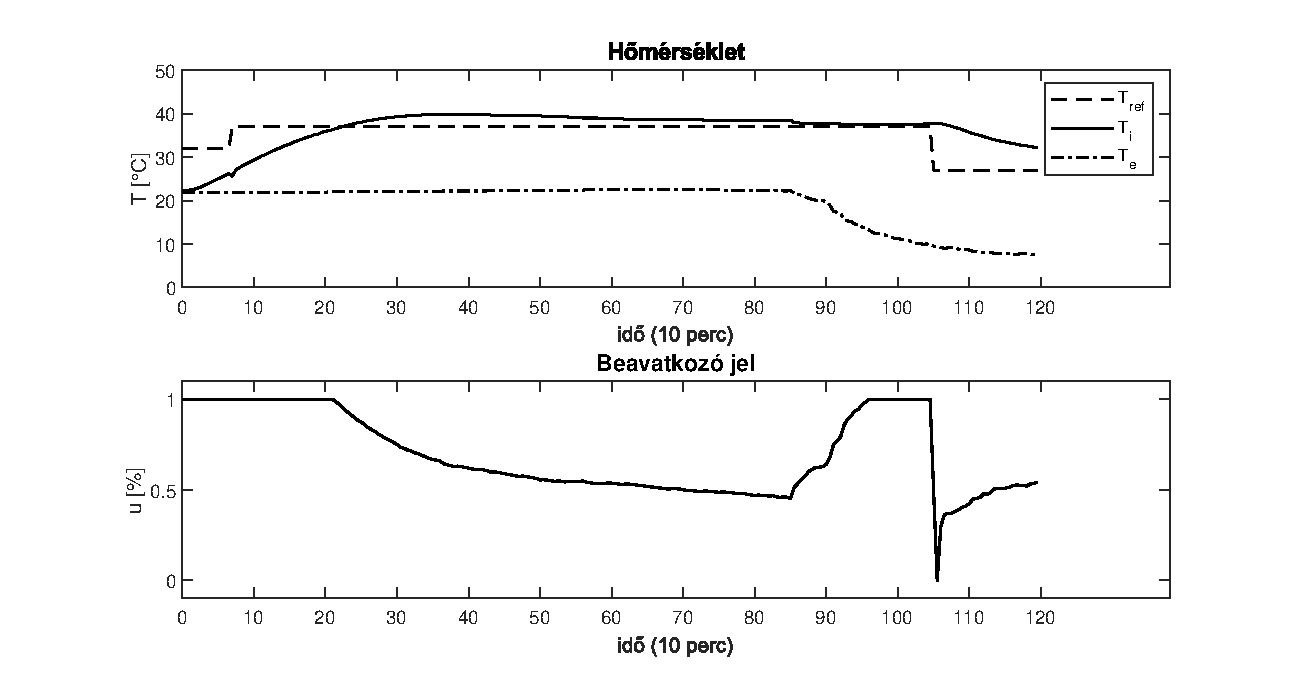
\includegraphics[width=0.95\textwidth]{figures/realsys/step}
	\caption{Mérés a fizikai rendszeren a behangolt MPC-vel}
	\label{fig:mpc-step}
\end{figure}

A tárgyaltakon felül további lehetőségek is vannak a költségfüggvények megadására. \textit{Thieblemont és Schirrer} \cite{SCHIRRER201686} megmutatta, hogy különösen jó eredmény érhető el MPC szabályozás és megújuló energiák kombinált használatával. A költségfüggvényekben például laza megkötéseket is lehet tenni, amik az adott jelet korlátozzák ugyan, de mégis túlléphetők - ilyenek egy napelemes rendszernél könnyen előfordulhatnak. Ekkor a laza felső korlát lehet a napelemes rendszer teljesítménye, de ezen felül is lehet energiát felhasználni a hálózatból.

Szintén \textit{Thieblemont} \cite{THIEBLEMONT2017485} készített felmérést az időjárás-előrejelzéssel kombinált MPC használatáról. (Itt a már korábban említett Signal Prevewing funkció használatos a jövőbeli bemenetek becsléséhez.) Az itt olvasható tapasztalatok és a bemutatott módszerek iránymutatást adhatnak a jövőbeni fejlesztésekhez.


%% Feljesztési lehetőségek
%\begin{formal}
%	Még lehetséges:
%	\begin{itemize}[noitemsep,topsep=-8pt,parsep=0pt,partopsep=0pt]
%		%		\item kazán bekapcsolása
%		%		\item előremenő hőmérséklet - unmeasured VAGY uncontrolled inputként
%		%		\item 1 db. fűtőtest (most radiátor) szelepének tömegárama (szelep áteresztése)
%		%		\item Később több fűtőtest vagy többféle fűtőtestek (padlófűtés, különböző teljesítményű radiátorok) szabályozása
%		\item környezeti hőmérséklet: predikció / szekvencia használata% is lesz rá. Hatása a kimeneten már identifikálva lett, 3 pólussal és 2 zérussal tökéletesen lekövethető.
%		\item napsugárzás zavaró hatása% - szimulálható  a bizonytalansága valószínűleg nagy lesz
%	\end{itemize}
%	
%	Belső változók - fűtési rendszer és ház kapcsolata
%	\begin{itemize}[noitemsep,topsep=-6pt,parsep=0pt,partopsep=0pt]
%		\item napsugárzás - radiatív, az ablak felületével és a szöggel arányos
%		\item fűtőtestek sugárzó és konvektív hőárama
%	\end{itemize}
%	
%	Paraméterek a plantben nem állandók:
%	\begin{itemize}[noitemsep,topsep=-6pt,parsep=0pt,partopsep=0pt]
%		%		\item hőátadási tényezők hőmérsékletfüggők, áramlási sebesség-függők (szél)
%		\item szellőztetés, belső hőterhelés hatása
%	\end{itemize}
%\end{formal}
\chapter{Gyakorlati megvalósítás lehetőségei}


\section{Technikai feltételek}\label{chap:feasibility-tech}

A legfontosabb technikai követelmény egy arányos szelep, ami a tömegáramot automatikusan, emberi beavatkozás nélkül képes befolyásolni. Ilyen például a Herz 7990\footnote{A szelep adatlapja: \url{http://herzmediaserver.com/data/01_product_data/01_datasheets/eng/7708-7990_en.pdf}}, \textit{Csoknyai} \cite{Herz} könyvében szerepelnek a Herz cég gépészeti termékei.

A Simulinkből történő hőmérsékletméréshez nagyon sok fejlesztésre volt szükség az iContrALL központi egységén. A rendszerbe való további integrációhoz ki kell dolgozni egy jobban skálázható megoldást (több hőmérő részére), ami meglehetősen időigényes. Ráadásul a hőmérők egyelőre egy külön központi egység közbeiktatásával kommunikálnak, ami nem teszi rugalmassá a használatot.
A beavatkozó jelek kiadása hasonló megfontolásokat igényel, integrációja ennek is időigényes.

Annak tehát, hogy egy helyiségenkénti hőmérséklet-szabályozás működjön, számos előfeltétele van. A felsoroltak pedig mind szoftveres, mind hardveres fejlesztéseket, beruházásokat igényelnek.

\section{Piaci lehetőségek}

A félévben lehetőségem volt az épületgépészettel gyakorlatban is találkozni, így jobban meg tudtam ítélni a bemutatott módszer piacképességét.

Ebben részben személyes tapasztalatokat mutatok be, amelyek nem tükrözik a teljes piac helyzetét (részben akár a trendekkel ellentétesek is lehetnek). Azzal, hogy betekintést nyertem az építőipar egy szegletébe, jobban el tudtam képzelni, mi a fizikai tartalom a sok technológia mögött, melyekkel az irodalomkutatás során találkoztam. Célom az volt, hogy képet szerezzek az alapvető elképzelésekről, elvárásokról egy HVAC rendszerrel szemben.

Egy nagy hazai kivitelező cég irodáinak látogatásakor figyeltem meg egy irodai környeztet. Arra voltam kíváncsi, adottak-e már a technikai feltételek egy ilyen szabályozás üzembe helyezéséhez, a konkrét irodában például az, hogy nagyobb átépítés nélkül\footnote{Azok a cégek, melyek azért építenek fel irodaházakat, hogy azokat bérbe adják, minél univerzálisabban szeretnének tervezni. Csak a központi magot, a szerkezeteket építik fel, a belsőépítészet, a \textit{héj} a bérlő igényei szerint valósul meg. Így előfordulhat, hogy bérlőcserekor átalakítják a bérlemény kinézetét, ekkor viszont alapvető épületgépészeti rendszerekhez nem nyúlnak hozzá.}, egy kész rendszerre is használható-e egy MPC szabályozás.

A meglátogatott épületben egy BMS (Building Management System) felügyelte a HVAC rendszereket. Ennek a géptermébe nem tudtam bemenni, de megfigyeltem az irodákban, a távhőközpontnál és a légkezelő egységeknél található gépészetet. A termosztátok és a távhőszelepek Johnson Controls gyártmányúak voltak.

Az irodákban a HVAC tervezésébe nagy mértékben beleszólt a nagy belső hőterhelés, ami a zsúfolt irodában megjelenik: a tervezők radiátoros fűtés mellett döntöttek, ezeket Danfoss elektronikus szelepek vezérlik. (Ezek pontos típusát nem tudom, de valószínűleg kétállásúak, és nem folytonosan szabályozhatók.) Szobánként lettek termosztátok elhelyezve. A szellőztetésről és a hűtésről Lindab Professional klímagerendák gondoskodnak. A BMS feladata, hogy egyszerre a fűtés és a hűtés ne legyen bekapcsolva. Az egész rendszer tervezése - igaz a főépítésszel és nem az épületgépész munkatárssal beszéltem - során a költséghatékonyságra és az alacsony karbantartási költségre törekedtek.

A technikai feltételekben a látottak alapján nem áll rosszul a piac, de ahhoz, hogy egy összetett szabályozásra költsenek egy épület tervezői, garanciát kellene adni az így elérhető megtakarításokra, amiket LEED vagy WELL tanúsítványokban extra pontokkal értékelnek.

%Külső árnyékolót sem használtak: korszerű ablakok használata mellett olyan alacsony a megtakarítás, hogy a megtérülési idő nagyon magas lett volna, illetve szélre érzékeny, karbantartást igénylő elem.
\input{src/optimality}
\chapter{Összefoglalás}

A félév során egy olyan témakörrel foglalkoztam, amihez szükség volt az alapképzés során szerzett összes rendszer- és irányításelméleti tudásra. Kellő hálózatelméleti szemlélettel az épületfizikai összefüggéseket szinte egy betűcserével be lehetett fogadni, hiszen a jelenségek analógok az elektromos hálózatokkal.

Számos tapasztalattal lettem gazdagabb a szabályozásokkal kapcsolatban is, a kutatómunka során rengeteg forrást áttekintettem. A tématerületbe való betekintés motivációt ad a mesterképzés tárgyaihoz is, mivel már ismerem az ilyen típusú szabályozók egyes gyakorlati alkalmazásait.


\chapter*{Köszönetnyilvánítás}
Köszönöm a segítséget és a motivációt konzulenseimnek, szüleimnek, munkatársaimnak. Az épületbejárás szervezéséért köszönet a BME Építész Klubnak.


\pagebreak
\bibliographystyle{unsrt}
\bibliography{szakdogaforras}

%\bibliography{szakdogaforras}
%%\addcontentsline{toc}{chapter}{Irodalomjegyzék}
%\bibliographystyle{plain}

%\include{appendices}

\label{page:last}
\end{document}
